\documentclass[review,3p,10pt,sort&compress]{elsarticle}
%\documentclass[preprint,5p,10pt,sort&compress]{elsarticle}

\usepackage{amsfonts,amsmath,amssymb,graphicx,dsfont,color}
\usepackage{multirow}
\usepackage[tight,normalsize,sf,sf]{subfigure}
\usepackage{epstopdf}

\journal{Signal Processing}
\linespread{1.25}

\begin{document}

\begin{frontmatter}

\title {Improved Pixel-based Pixel-Value-Ordering High-fidelity Reversible Data Hiding}

\author{Haorui Wu}
\ead{hrwu@bjtu.edu.cn}

\author{Xiaolong Li}
\ead{lixl@bjtu.edu.cn}

\author{Yao Zhao\corref{cor}}
\cortext[cor]{Corresponding author. Tel./Fax:  +86 10 51688667.}
\ead{yzhao@bjtu.edu.cn}

\author{Rongrong Ni}
\ead{rrni@bjtu.edu.cn}

\address[mymainaddress]{Institute of Information Science, Beijing Jiaotong University, Beijing 100044, China}
\address[mysecondaryaddress]{Beijing Key Laboratory of Advanced Information Science and Network Technology, Beijing 100044, China}

\begin{abstract}
Pixel-value-order(PVO) is a high-fidelity reversible data hiding (RDH) method which is commonly used today. Traditional PVO-based RDH methods first divide the cover image into blocks and data is embedded into prediction-errors of the largest/smallest pixels block-by-block. Later, the pixel-based PVO(PPVO) is proposed by the motivation of overcoming the block constraint. Each pixel is predicted by the neighbor sorted context pixels and the number of context pixels of each pixel to-be-predicted is constant. In this paper, a extended PPVO-based RDH method is proposed with a extended PPVO predictor and embedding procedure is implemented by a multi-size based embedding method. First, a extended PPVO predictor is proposed to further utilize the surrounding context information to obtain a sharper prediction-error histogram(PEH). Then, we explore the impact of the various sizes of context region. By considering the between local complexity, data is embedded into the prediction-error based on a suitable context region size. The experimental results shows that the proposed method achieve outstanding performances and is superior to several state-of-the-art PVO-based methods.
\end{abstract}


\begin{keyword}
   Reversible data hiding\sep pixel-value-ordering\sep adaptive embedding\sep multiple histograms modification
\end{keyword}

\end{frontmatter}

%----------------------------------------------------------------------------------------
\section{Introduction}\label{sec:1}
% RDH PEH PVO MHM
In recent days, the tampering and dissemination of multimedia data have been getting more and more convenient. In order to verify the integrity and security of information, technologies such as information encryption, fingerprint recognition and data hiding have been extensively studied. Among them, reversible data hiding(RDH) is a technology that embeds secret data into image in an imperceptible way and the decoder can recover the original content lossless from the marked image while extracting the secret data.

Up to now, RDH has been extensively explored and many types of techniques such as difference expansion(DE), histogram shifting(HS) and prediction-error expansion(PEE) have emerged. Among the techniques, the first DE-based method is proposed by Tian \emph{et al.} which expands the difference between adjacent pixels to achieve embedding procedure. By embedding data into the differences, the high fidelity is guaranteed. HS-based methods achieve embedding by shifting pixels according to the peak-gap distribution of image histogram. However, embedding capacity and distortion is mainly sensitive to characteristic of the histogram. Besides, unlike DE-based and HS-based methods, PEE is the most influential RDH technique due to its balance between distortion and capacity. PEE is first proposed by Thodi and Rodriguez in .... In this PEE-based method, pixels are first predicted by adjacent pixels and then accurately predicted pixels are modified by expanding the prediction-errors for embedding, while the others are shifted to ensure the reversibility. Focus on the pixel prediction or modification of prediction-errors, many methods are proposed, e.g., accurate predictor design for prediction-error histogram(PEH), high-dimension histogram modification and multiple histogram modification(MHM).

Among the PEE-based methods, pixel-value-order(PVO) is the most critical technology which provides an accurate prediction method. The original PVO-based method is proposed by Li \emph{et al.}. For the data embedding, the cover image is first divided into equal size and non-overlapping blocks. Then, in each block, the pixels are sorted in an ascending order. And the largest/smallest pixel value is predicted by the second largest/smallest pixel value to derive the prediction-error. At last, for the generated PEH, a expansion/shift modification is carried out on each prediction-error for embedding. In the original PVO-based RDH, it is note that smooth blocks can not be used for embedding. Due to this reason, Peng \emph{et al.} propose an improved PVO method which considers the original order of the largest/smallest pixel value and the second the largest/smallest pixel value, resulting in the fully utilized of smooth blocks. Meanwhile, Ou \emph{et al.} propose the PVO-$k$ scheme which modifies the first several largest/smallest pixel values at the same time to overcome the same shortage. Furthermore, Qu \emph{et al.} notice that lots of pixels are omitted in embedding procedure because of the block constraint. Thus, they proposed a pixel-based PVO method. The target pixel is predicted by the the largest/smallest neighbor context pixels and it gets a high embedding capacity by the pixel-by-pixel strategy.
In addition, from the same motivation, Wang \emph{et al.} divide the cover image into two size blocks due to the region complexities, and further exploit the correlation of pixels in smooth regions.

In this paper, we try to improve the performance of PPVO RDH. First, we find that in the original PPVO RDH method, part of surrounding context pixels do not appreciate in the prediction process, which are also correlated with the pixel to-be-predicted. In this work, a extended PPVO predictor is proposed which utilizes pixels in left lower direction of target pixel for prediction as well. And it carries out an accurate prediction process to derive a sharper PEH. Meanwhile, the impact of various size of context region is explored. The context region size is chosen by the local complexity of the target pixel. Pixels in smooth area are predicted with a small context region size and pixels in complex area are predicted with a larger size. The experimental results verify that the proposed method is superior to the several state-of-the-art PVO-based methods.

The rest of the paper is arranged as follow. Section \ref{sec:2} is a brief review of the two classical PVO-based RDH methods. Section \ref{sec:3} is the introduction of the proposed extended pixel-based PVO method. Section \ref{sec:4} shows the experimental results. Finally, Section \ref{sec:5} concludes the paper.

%----------------------------------------------------------------------------------------
\section{Related Works}\label{sec:2}
In this section, as prior knowledge, we will review the improved PVO-based RDH method of Peng \emph{et al.} \cite{Peng2014IPVO} and the Pixel-based PVO RDH(PPVO) method of Qu \emph{et al.} \cite{Qu2015PPVO}. And the data embedding amd extraction procedures are presented followed.

\subsection{Improved PVO-based RDH \cite{Peng2014IPVO}}\label{sec:2.1}
In original PVO-based method \cite{Li2013PVO} of Li \emph{et al.}, first, the cover image is divided into equal size and non-overlapping blocks with size of $n = a \times b$. And then pixels $(x_{1},...,x_{n})$ in the given block is sorted in ascending by the pixel values, to obtained $(x_{\xi(1)},...,x_{\xi(n)})$, where $\xi : \{1,...,n\} \rightarrow \{1,...,n\}$ is the one-to-one mapping which respecting the rules of $\xi(i) < \xi(j)$ if $x_{i} = x_{j}$ ($i < j$). Then, the largest pixel $x_{\xi(n)}$ is predicted by the second largest pixel $x_{\xi(n-1)}$ and the prediction-error of $x_{\xi(n)}$ is defined as $p_{\rm max} = x_{\xi(n)} - x_{\xi(n-1)}$, where the prediction-error is subject to the interval of $[0, \infty)$ due to the truth $x_{\xi(n)} \geq x_{\xi(n-1)}$. In this method, $p_{\rm max} = 1$ appears  most often so that prediction-errors of $p_{\rm max} = 1$ are expanded to embed data while others of $p_{\rm max} > 1$
%(while other blocks)
are shifted to ensure reversibility. However, in original PVO-based RDH, blocks of $p_{\rm max} = 0$ are not used which are usually smooth and beneficial for reversible embedding. Based on this motivation, Peng \emph{et al.} propose an improved PVO-based RDH method \cite{Peng2014IPVO}.

In the improved PVO-based RDH method, for each block, the computation of $p_{\rm max}$ is redefined by considering the order of $\xi(n-1)$ and $\xi(n)$ as
\begin{equation}\label{eq:pmax}
p_{\rm max} = \left\{\begin{array}{ll}
x_{\xi(n)} - x_{\xi(n-1)},      & \text{if } \xi(n) > \xi(n-1) \\
x_{\xi(n)} - x_{\xi(n-1)} - 1,  & \text{if } \xi(n) < \xi(n-1)
\end{array}\right.,
\end{equation}
where the prediction-errors $p_{\rm max} \geq 0$ locating in the interval of $[0, \infty)$ as well.

The different of improved PVO-based method and original PVO-based method is that a part of blocks whose prediction-errors large than 1 in original method, i.e., $x_{\xi(n)}-x_{\xi(n-1)} \geq 1$, but with the order $\xi(n) < \xi(n-1)$, are recomputed to $x_{\xi(n)} - x_{\xi(n-1)} - 1$, resulting the PEH peaking at 0 instead of 1 in \cite{Li2013PVO}. For example, PEH of the standard gray-scale image Lena is shown as Fig. \ref{Fig.PVOIPVO}.
\begin{figure*}
%    \centering
%    \subfigure{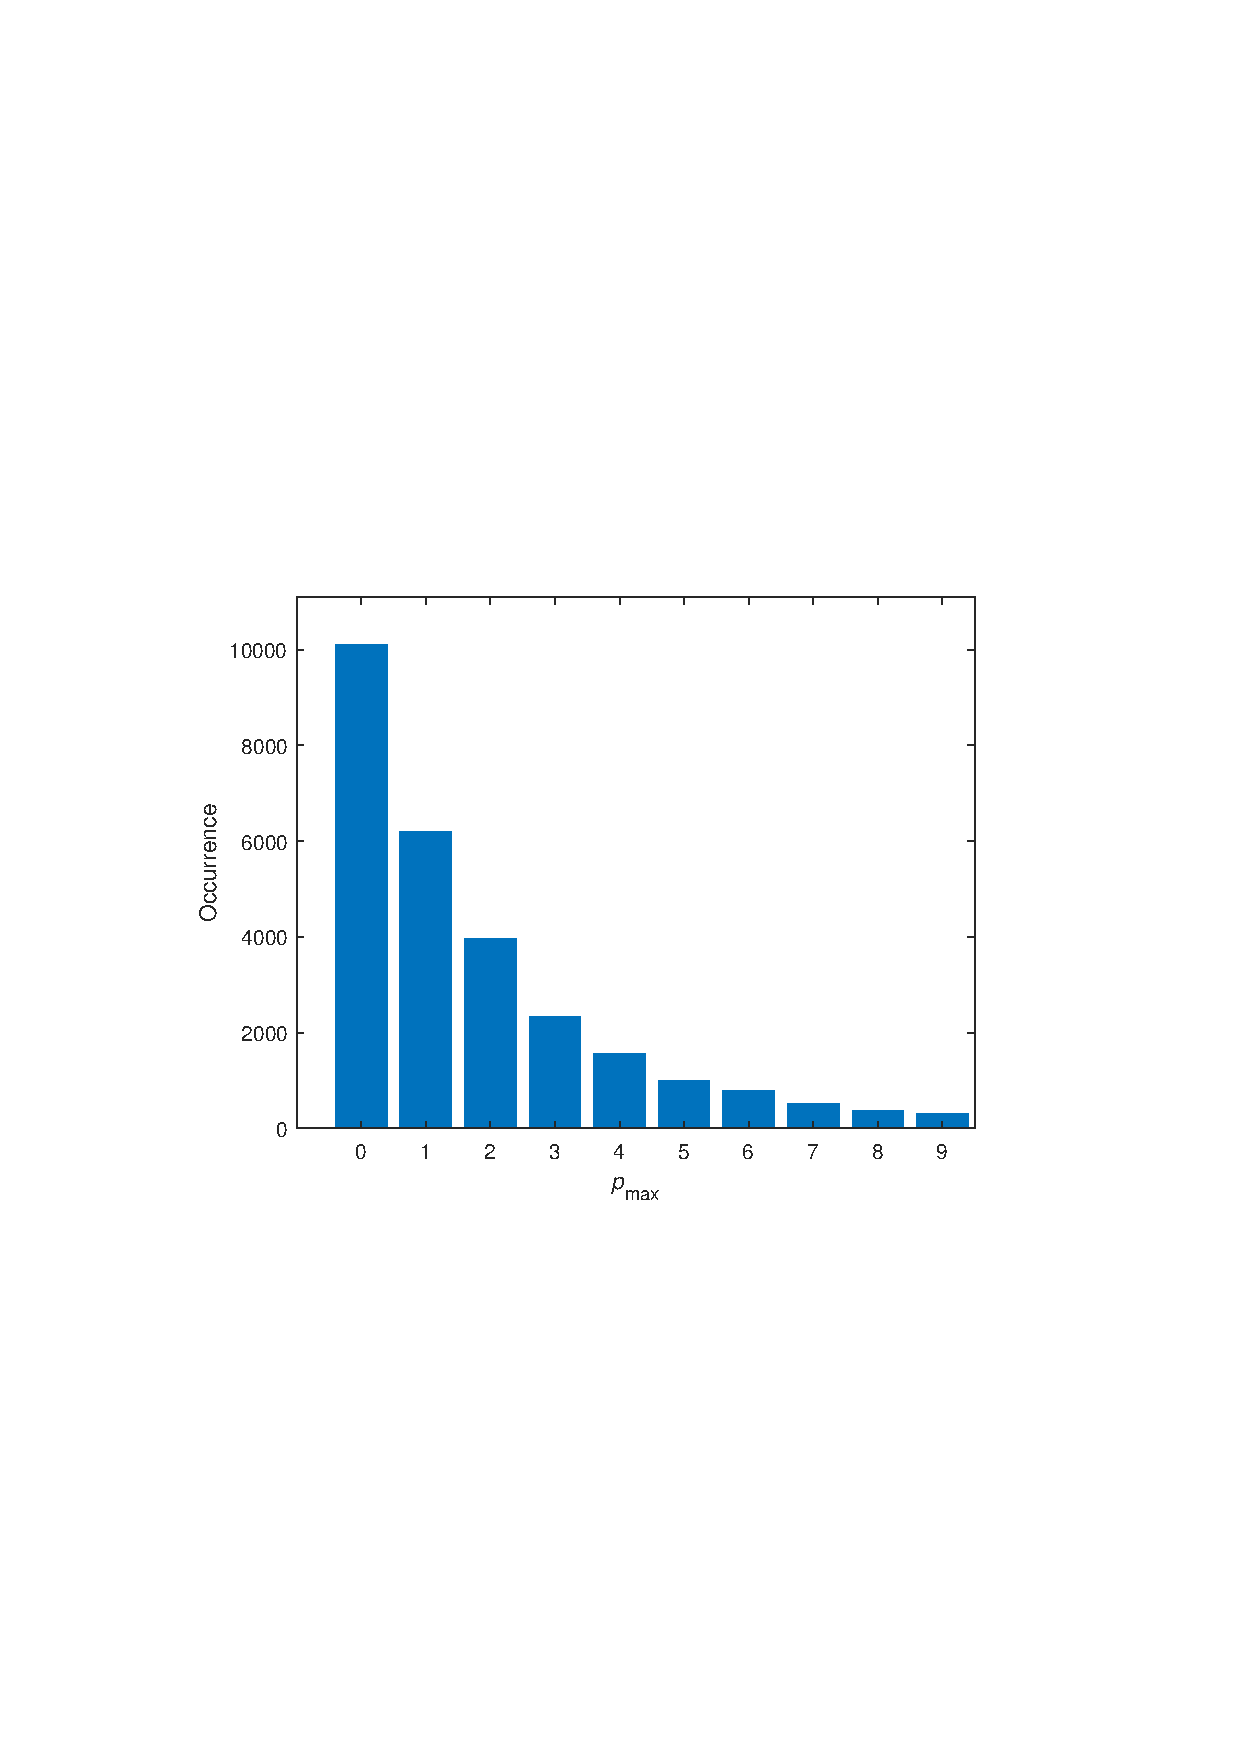
\includegraphics[width=0.35\textwidth]{figures/IPVO_Lena_3x3_hist.pdf}}
%    \caption{PEH of $p_{\rm max}$ by \eqref{eq:pmax} for the standard gray-scale $512 \times 512$ sized image Lena.}
%    \label{Fig.IPVO}
\centering
\subfigure[Original PVO-based method \cite{Li2013PVO}.]{
    \begin{minipage}[t]{0.32\linewidth}
    \centering
    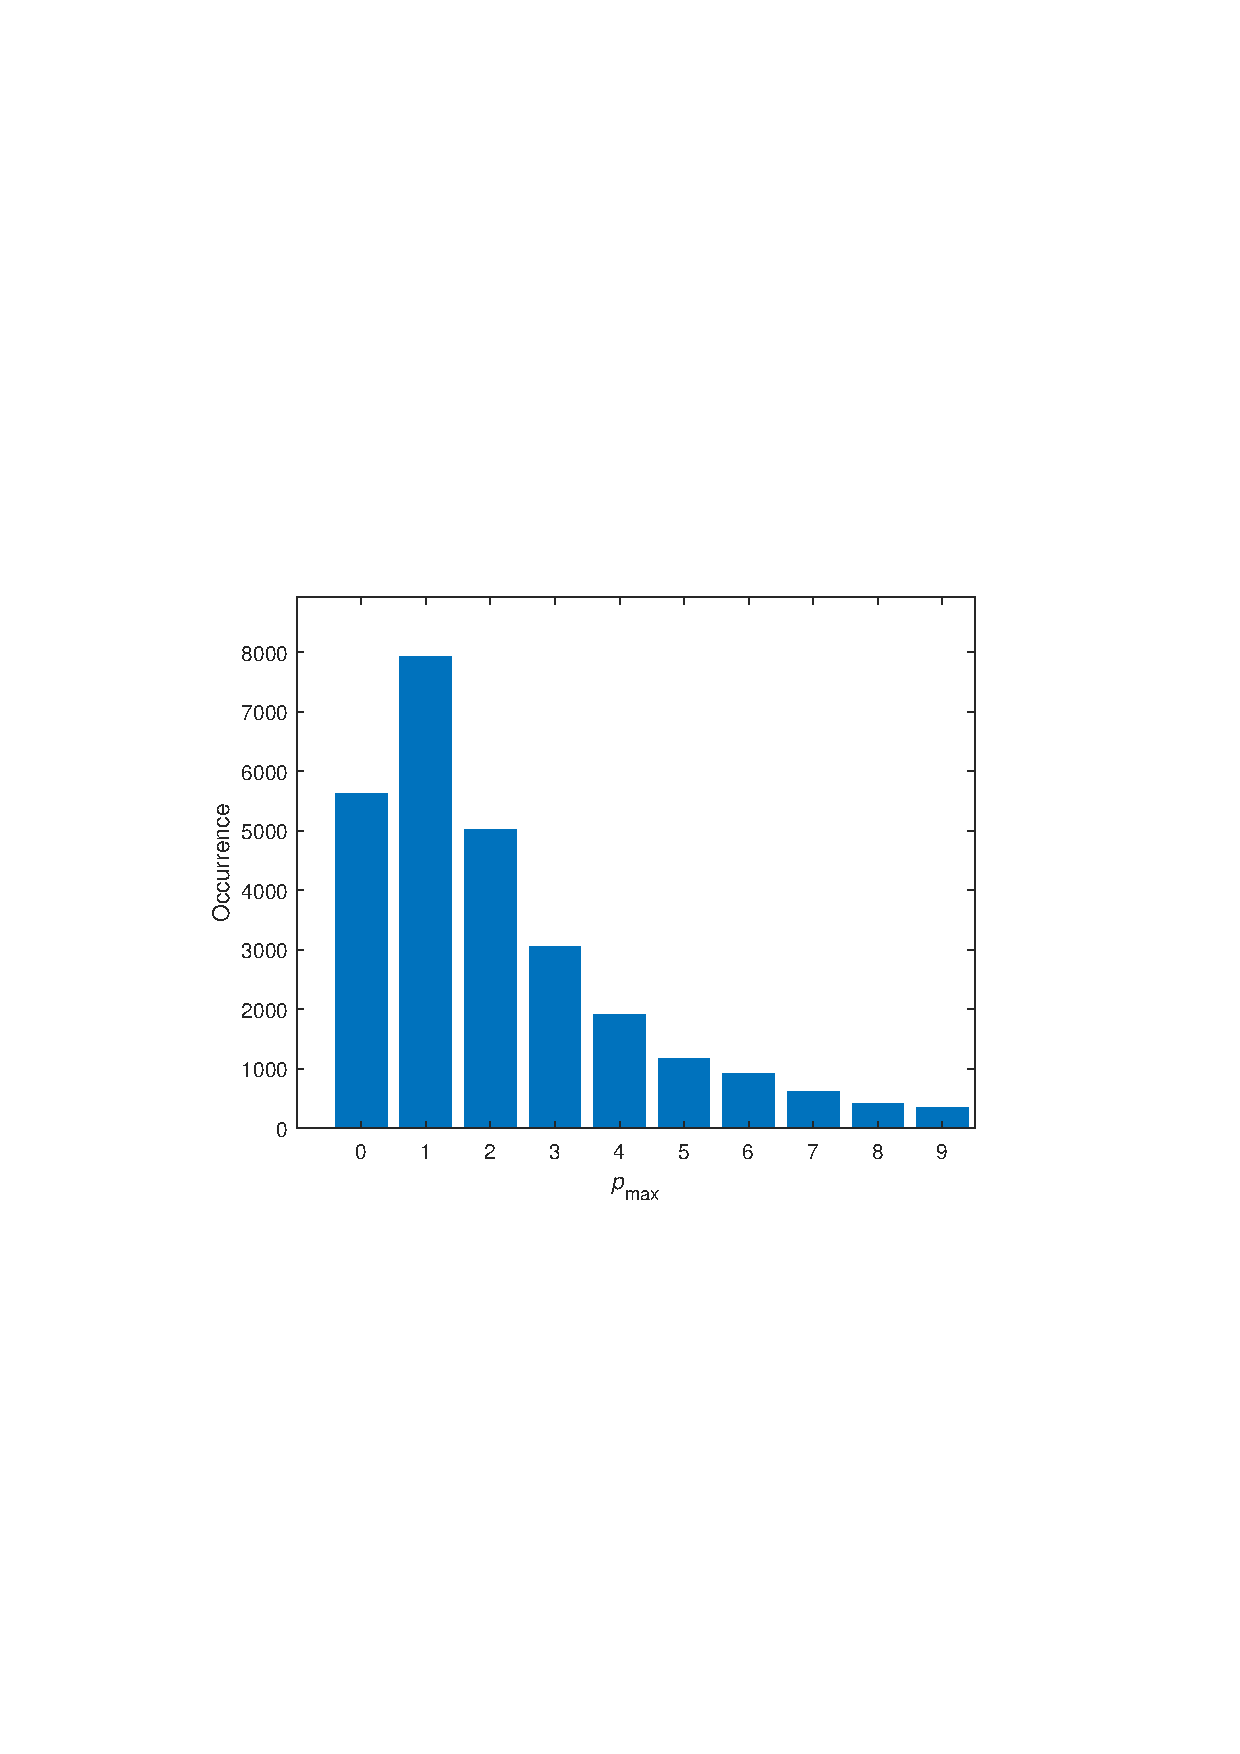
\includegraphics[width=1\textwidth]{figures/PVO_Lena_3x3_hist.pdf}
    \end{minipage}
}
\qquad\qquad
\subfigure[Improved PVO-based method \cite{Peng2014IPVO}.]{
    \begin{minipage}[t]{0.33\linewidth}
    \centering
    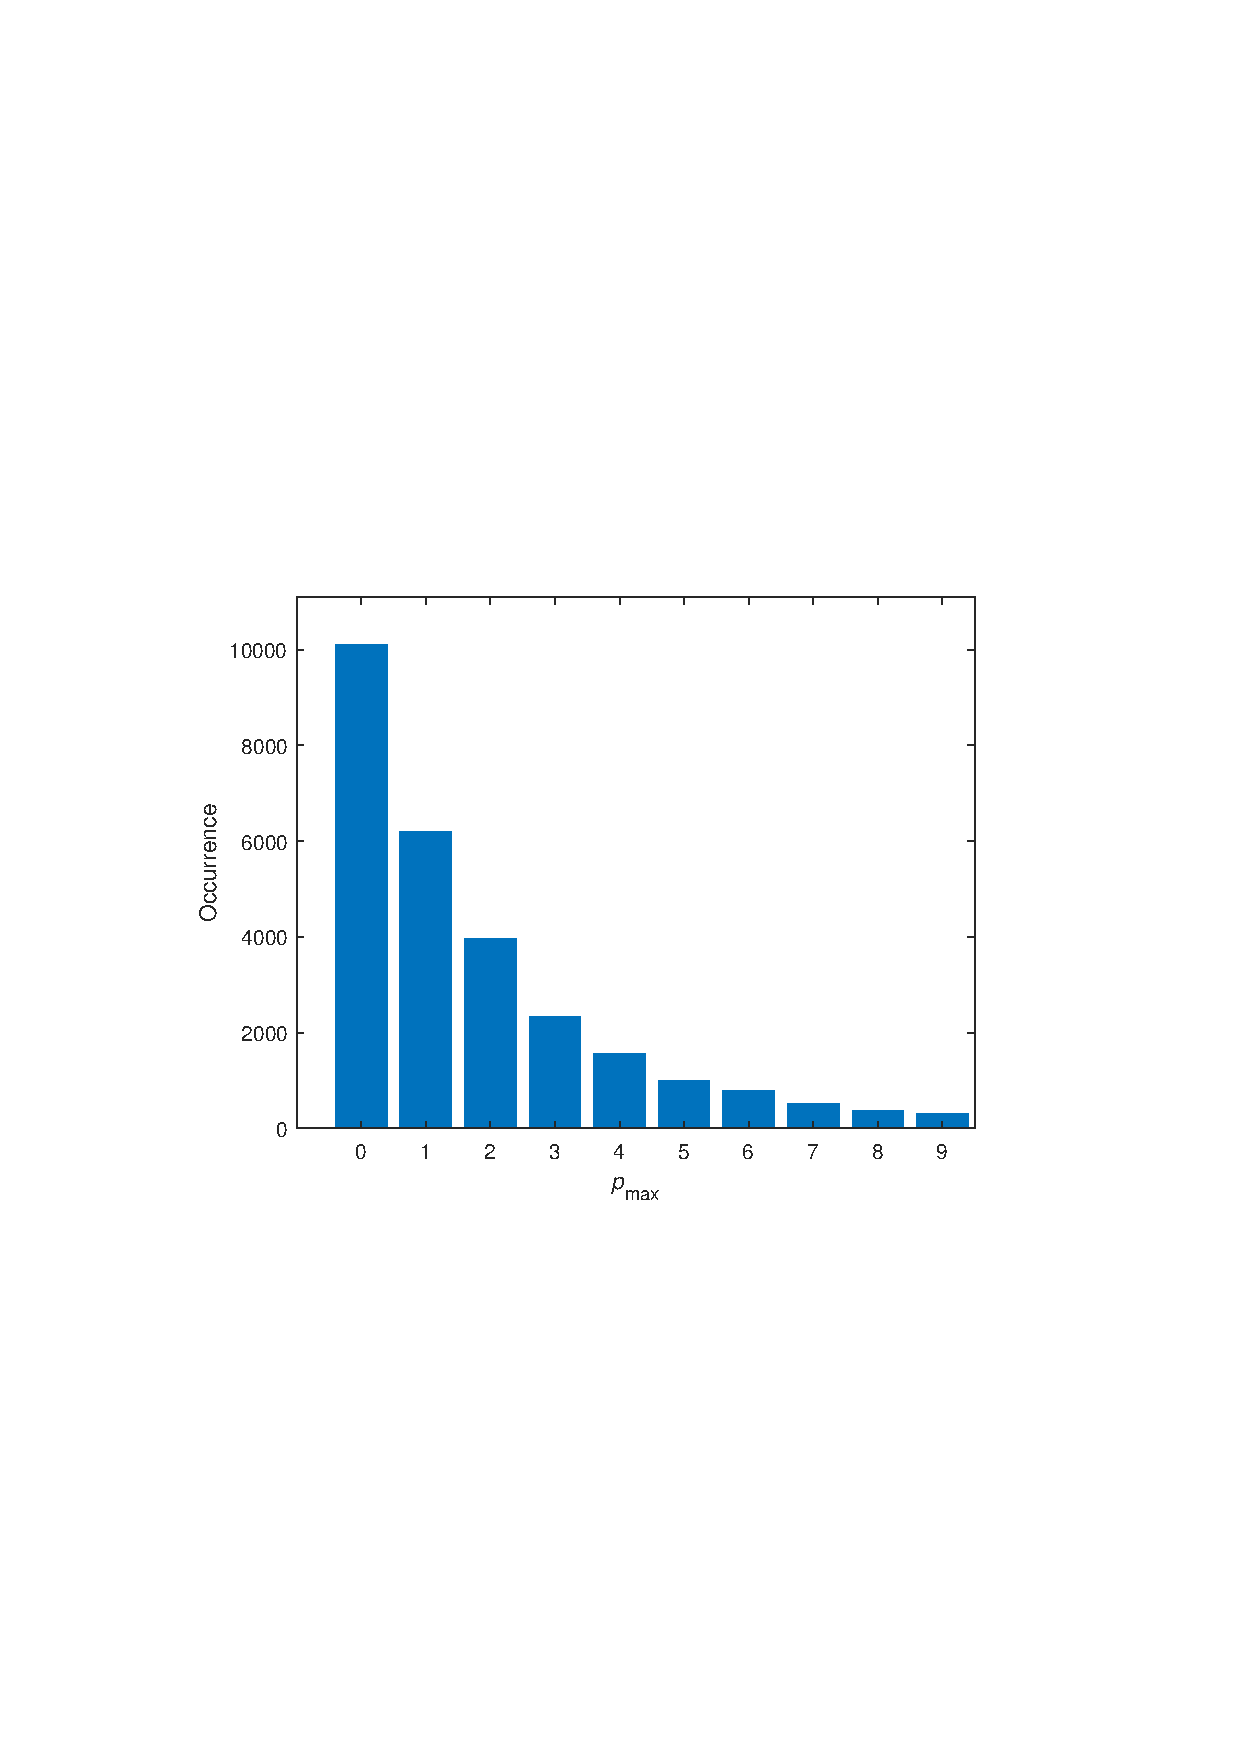
\includegraphics[width=1\textwidth]{figures/IPVO_Lena_3x3_hist.pdf}
    \end{minipage}
}		
\centering
\caption{PEH of $p_{\rm max}$ with block size $n = 3 \times 3$ for the standard gray-scale $512 \times 512$ sized image Lena.}
\label{Fig.PVOIPVO}
\end{figure*}

More clearly, prediction-error $p_{\rm max}$ is modified to derive the marked prediction-error $\hat{p}_{\rm max}$ by
\begin{equation}\label{eq:mpmax}
\hat{p}_{\rm max} = \left\{\begin{array}{ll}
p_{\rm max} + b, & \text{if } p_{\rm max}=0 \\
p_{\rm max} + 1, & \text{if } p_{\rm max}\geq 1 \\
\end{array}\right.,
\end{equation}
where $b \in \{0,1\}$ is one bit secret data to be embedded. And, the marked largest pixel $\hat{x}_{\xi(n)}$ is obtained by
\begin{equation}\label{eq:mpixel}
\hat{x}_{\xi(n)} = x_{\xi(n-1)} + \hat{p}_{\rm max}.
\end{equation}
In the improved PVO-based method, in each block, it is note that $\hat{x}_{\xi(n)} \geq x_{\xi(n)}$, and the PVO of the marked pixels $(\hat{x}_{\xi(1)},...,\hat{x}_{\xi(n)})$ is as the same as the original pixels, which guarantees the reversibility.

For the decoder, in each block, the marked prediction-error $\hat{p}_{\rm max}$ with pixels $(\hat{x}_{\xi(1)},...,\hat{x}_{\xi(n)})$ in ascending order is computed as
\begin{equation}\label{eq:dmpmax}
\hat{p}_{\rm max} = \left\{\begin{array}{ll}
\hat{x}_{\xi(n)} - \hat{x}_{\xi(n-1)},      & \text{if } \xi(n) > \xi(n-1) \\
\hat{x}_{\xi(n)} - \hat{x}_{\xi(n-1)} - 1,  & \text{if } \xi(n) < \xi(n-1)
\end{array}\right.,
\end{equation}
Next, the original pixel value $x_{\xi(n)}$ is recovered by
\begin{equation}\label{eq:dmpixel}
x_{\xi(n)} = \left\{\begin{array}{ll}
\hat{x}_{\xi(n)},       & \text{if } \hat{p}_{\rm max} = 0 \\
\hat{x}_{\xi(n)} - 1,   & \text{if } \hat{p}_{\rm max} \geq 1 \\
\end{array}\right.,
\end{equation}
while other marked pixels $(\hat{x}_{\xi(1)},...,\hat{x}_{\xi(n-1)})$ is recovered as themselves. And, the embedded secret data is 0 if $\hat{p}_{\rm max} = 0$ and 1 if $\hat{p}_{\rm max} = 1$.

Moreover, for each block, the similar process is applied to the smallest pixel value $x_{\xi(1)}$ by computing the prediction-error $p_{\rm min}$ as
\begin{equation}\label{eq:pmin}
p_{\rm min} = \left\{\begin{array}{ll}
x_{\xi(2)} - x_{\xi(1)},      & \text{if } \xi(2) > \xi(1) \\
x_{\xi(2)} - x_{\xi(1)} - 1,  & \text{if } \xi(2) < \xi(1)
\end{array}\right.,
\end{equation}
where pixel $p_{\rm min} \geq 0$. And the PEH of $p_{\rm min}$ peaks at 0 as well. The detail embedding and extraction process is described in \cite{Peng2014IPVO}.


\subsection{Pixel-based PVO RDH \cite{Qu2015PPVO}}\label{sec:2.2}
In the classical PVO-based RDH method such as the original PVO-base method \cite{Li2013PVO} and the improved PVO-based method \cite{Peng2014IPVO}, the cover image is first devided into equal size and non-overlapping blocks. The sorted pixels $(x_{\xi(2)},...,x_{\xi(n-1)})$ is not utilized in the embedding process and the total number of prediction-errors is bounded by the block constraint, which causing the difficulty of efficient embedding data into smooth region. In \cite{Qu2015PPVO}, Qu \emph{et al.} propose a pixel-based PVO RDH method, which is called PPVO, to utilized the sorted pixels for data embedding.

PPVO achieves an pixel-by-pixel data embedding process. For current pixel, the context pixels defined as the pixels in the lower right direction and form an vector $C=\{c_1,...,c_{\rm CN}\}$ shown in Fig. \ref{Fig.PPVOCNandHist}(a), where the number of context pixels is defined as ${\rm CN}$.
\begin{figure*}
\centering
\subfigure[Context pixels of $x$.]{
    \begin{minipage}[t]{0.22\linewidth}
    \centering
    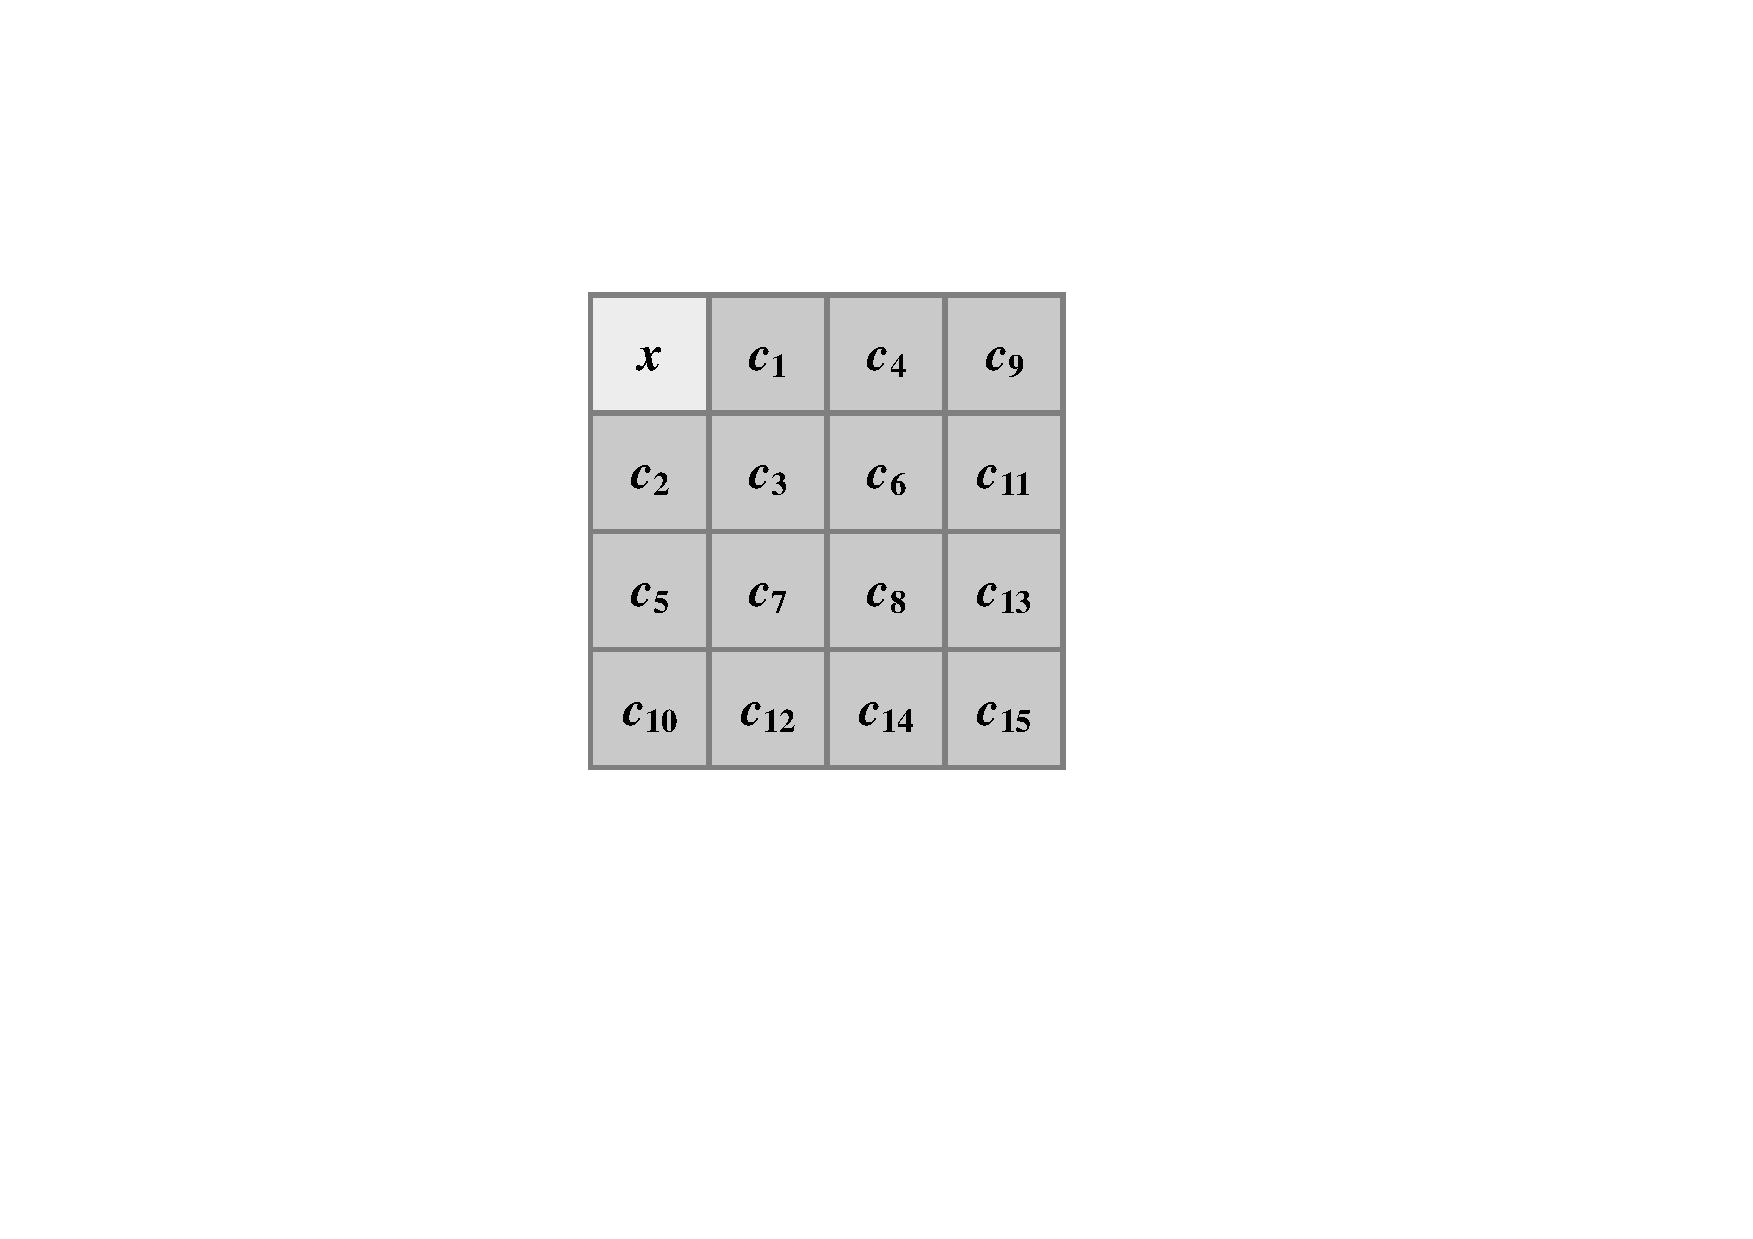
\includegraphics[width=1\textwidth]{figures/PPVOContext.pdf}
    \end{minipage}
}
\qquad\qquad\qquad
\subfigure[PEH of $p$ by \eqref{eq:PPVOPE}.]{
    \begin{minipage}[t]{0.31\linewidth}
    \centering
    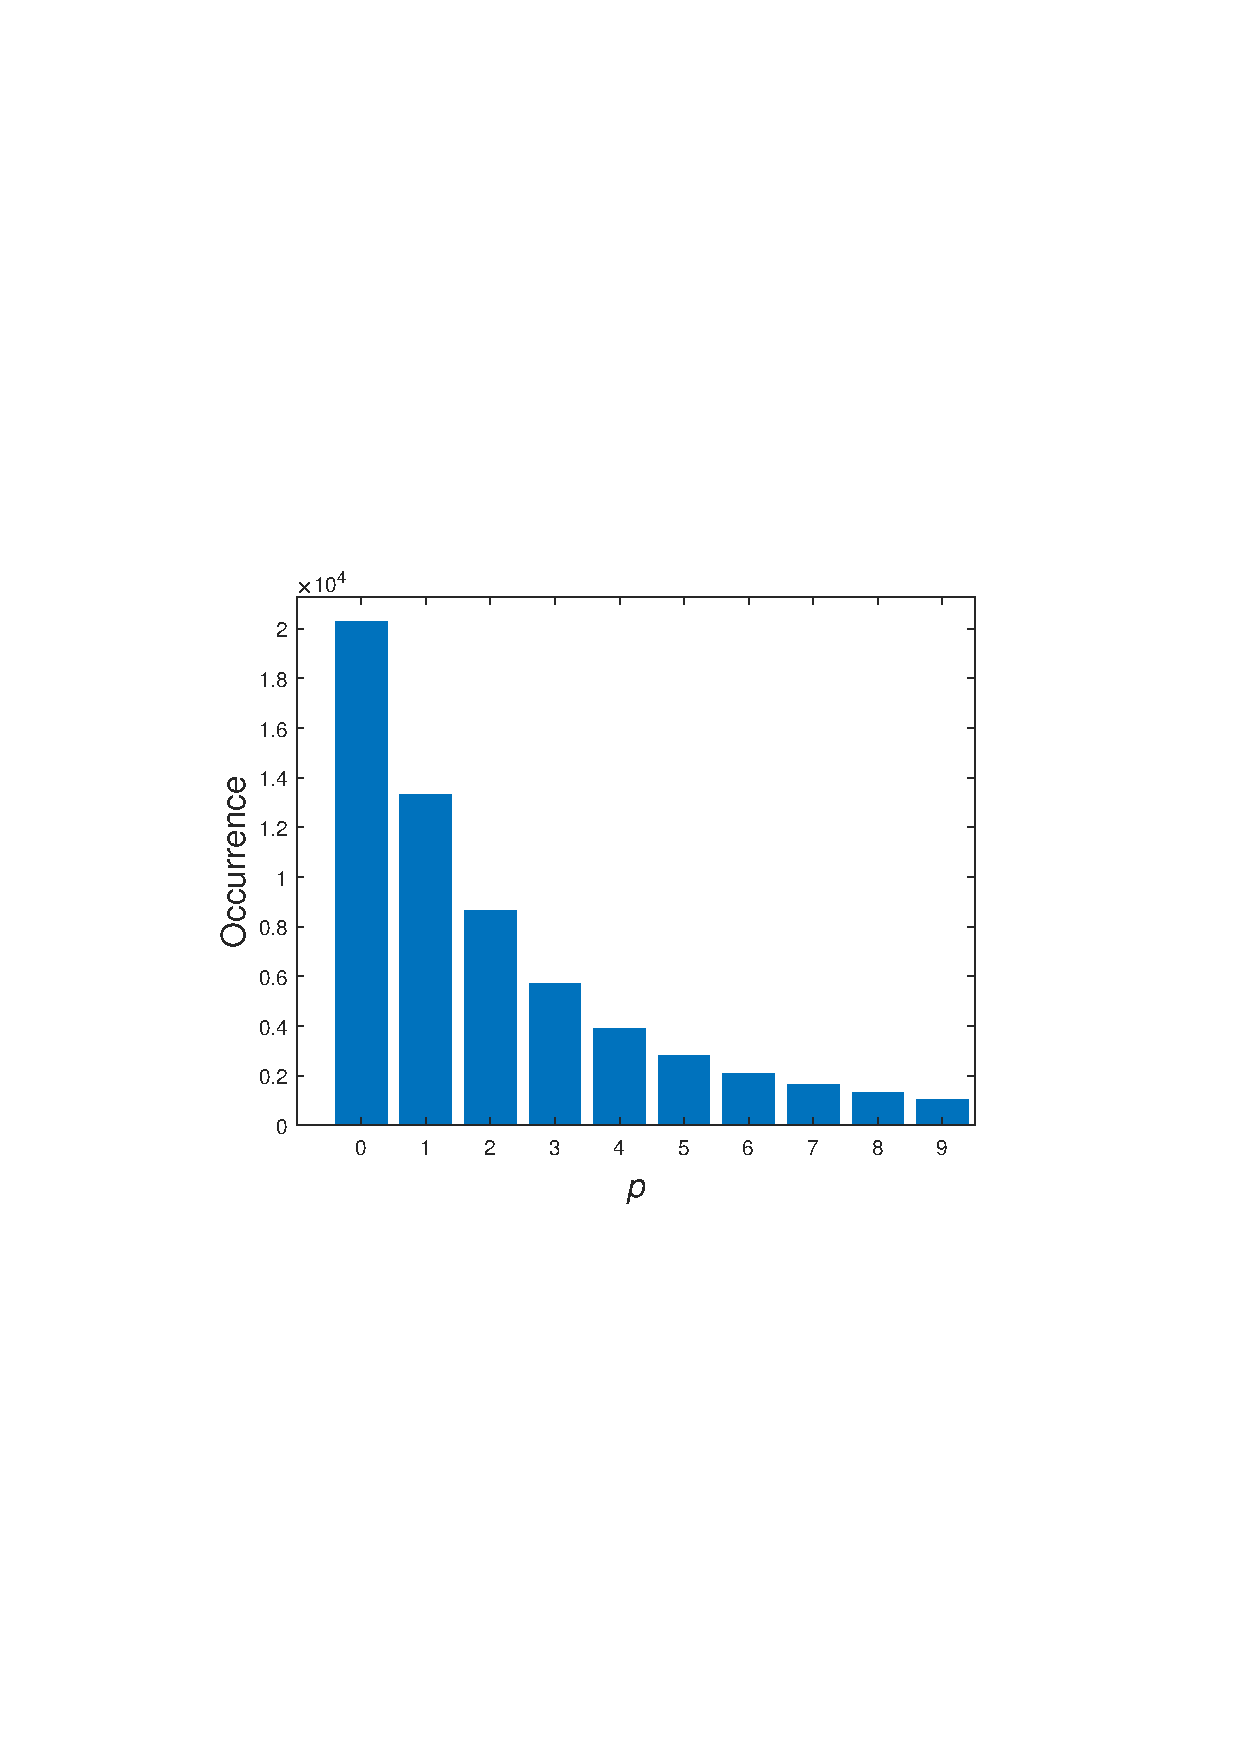
\includegraphics[width=1\textwidth]{figures/PPVO_Lena_CN15_hist.pdf}
    \end{minipage}
}		
\centering
\caption{PPVO Context Pixels and show the shaper histogram with $CN = 15$.}
\label{Fig.PPVOCNandHist}
\end{figure*}

Before describe the prediction algorithm, to simplify the explanation, pixels participating in the embedding process are grouped into four sets, which are
\begin{equation*}\label{eq:S}
\begin{array}{ll}
S_1 = \{ x | \max(C) \neq \min(C), x \geq \max(C) \} \\
S_2 = \{ x | \max(C) \neq \min(C), x \leq \min(C) \} \\
S_3 = \{ x | \max(C)   =  \min(C), x \leq \min(C), \min(C) \neq 254 \} \\
S_4 = \{ x | \max(C)   =  \min(C), x \geq \min(C), \min(C) =  254 \} \\
\end{array}.
\end{equation*}
Then, for each pixel $x$, the prediction-error $p$ is calculated by
\begin{equation}\label{eq:PPVOPE}
p = \left\{\begin{array}{ll}
x - \max(C),    & \text{if } x \in S_1  \\
\min(C) - x,    & \text{if } x \in S_2 \cup S_3 \\
0,              & \text{if } x \in S_4 \\
{\rm skip},     & \text{otherwise}
\end{array}\right.,
\end{equation}
where prediction-error $p$ is located in the interval of $[0, \infty)$. More specifically, PEH of $p$ peak at 0 as shown in Fig. \ref{Fig.PPVOCNandHist}(b) so that $p$ is modified to derive the marked prediction-error $\hat{p}$ by
\begin{equation}\label{eq:PPVOMPE}
\hat{p} = \left\{\begin{array}{ll}
p + b,  & \text{if } p = 0      \\
p + 1,  & \text{if } p \geq 1
\end{array}\right.,
\end{equation}
where $b \in \{0,1\}$ is one bit secret data to be embedded. And the marked pixel $\hat{x}$ is obtained by
\begin{equation}\label{eq:PPVOMPixel}
\hat{x} = \left\{\begin{array}{ll}
\max(C) + \hat{p},  & \text{if } x \in S_1 \\
\min(C) - \hat{p},  & \text{if } x \in S_2 \cup S_3 \\
\min(C) + \hat{p},  & \text{if } x \in S_4 \\
{\rm skip},         & \text{otherwise}
\end{array}\right..
\end{equation}

In this method, for each pixel satisfying $x \notin S_4$, marked pixel satisfies $\hat{x} \geq x$ if $x \geq \max(C)$ and $\hat{x} \leq x$ if $x \leq \min(C)$ which ensures reversibility.
And reason of processing the pixels $x \in S_4$ specially is that pixels equal 255 are modified to 254 during the location map stage and $x \in S_4$ is increased by 1 or 0 can decrease the distortion of data embedding. It is note that, in the embedding process, the proper $NC$ is selected by choosing the best result of $C = \{1,...,i\}(i \in {1,...,15})$ exhaustively.

For the decoder, to extract data and recover the ordinal pixel, the same marked prediction-error $\hat{p}$ of current pixel $x$ is calculated by
\begin{equation}\label{eq:PPVOdMinNeqMax}
\hat{p} = \left\{\begin{array}{ll}
\hat{x} - \max(C),  & \text{if } \hat{x} \in S_1  \\
\min(C) - \hat{x},  & \text{if } \hat{x} \in S_2 \cup S_3 \\
\hat{x} - \min(C),  & \text{if } \hat{x} \in S_4  \\
{\rm skip},         & \text{otherwise}
\end{array}\right..
\end{equation}
In addition, the original pixel value $x$ is recovered by
\begin{equation}\label{eq:PPVOdMPixel}
x = \left\{\begin{array}{ll}
\hat{x},        & \text{if } \hat{p} = 0 \\
\hat{x} - 1,    & \text{if } \hat{x} \in S_1 \cup S_4 \text{ and } \hat{p} \geq 1 \\
\hat{x} + 1,    & \text{if } \hat{x} \in S_2 \cup S_3 \text{ and } \hat{p} \geq 1 \\
{\rm skip},         & \text{otherwise}
\end{array}\right..
\end{equation}
With the recover process, the secret data is extracted that $b = 1$ if $\hat{p}=1$ and $b = 0$ if $\hat{p} = 0$.

The experimental results show that PPVO gets a large maximum embedding capacity than the previous PVO-based method \cite{Li2013PVO,Peng2014IPVO} by pixel-by-pixel embedding. And it obtains a sharper histogram which is causing a result of better performance as shown in Fig. \ref{Fig.PPVOCNandHist}.

%----------------------------------------------------------------------------------------
\section{Proposed Method}\label{sec:3}
% motivation and simply description
In this section, a extended PPVO predictor is first introduced. Then, a multi-size based embedding method for MHM is proposed to further improve the performance. Finally, the embedding procedure and extraction procedure is described.

\subsection{Extended PPVO predictor}\label{sec:3.1}
Compared with PVO-based methods such as PVO\cite{Li2013PVO}, IPVO\cite{Peng2014IPVO} and PVO-\emph{k}\cite{Ou2014PVOk}, in PPVO, every pixel is predicted by context pixels, breaking through the block constraint. In PPVO, to ensure reversibility, pixels in lower right direction are utilized as context region to predict the current pixel which is shown in Fig. \ref{Fig.Context}(a). The prediction is more accurate, however, the surrounding context information is not fully utilized. There are some other pixels are omitted which is beneficial to provide more useful information for prediction. Clearly, for example, in Fig. \ref{Fig.Context}(b), pixels $\{c_{4}, c_{9}, c_{10}, c_{12}, c_{17}, c_{18}, c_{21}, c_{22}, c_{24}\}$ in left lower direction should be used in prediction procedure as one part of context pixels which is omitted in PPVO. Then the extended PPVO predictor is introduced to show how to make better prediction.
\begin{figure*}
\centering
\subfigure[PPVO.]{
    \begin{minipage}[t]{0.21\linewidth}
    \centering
    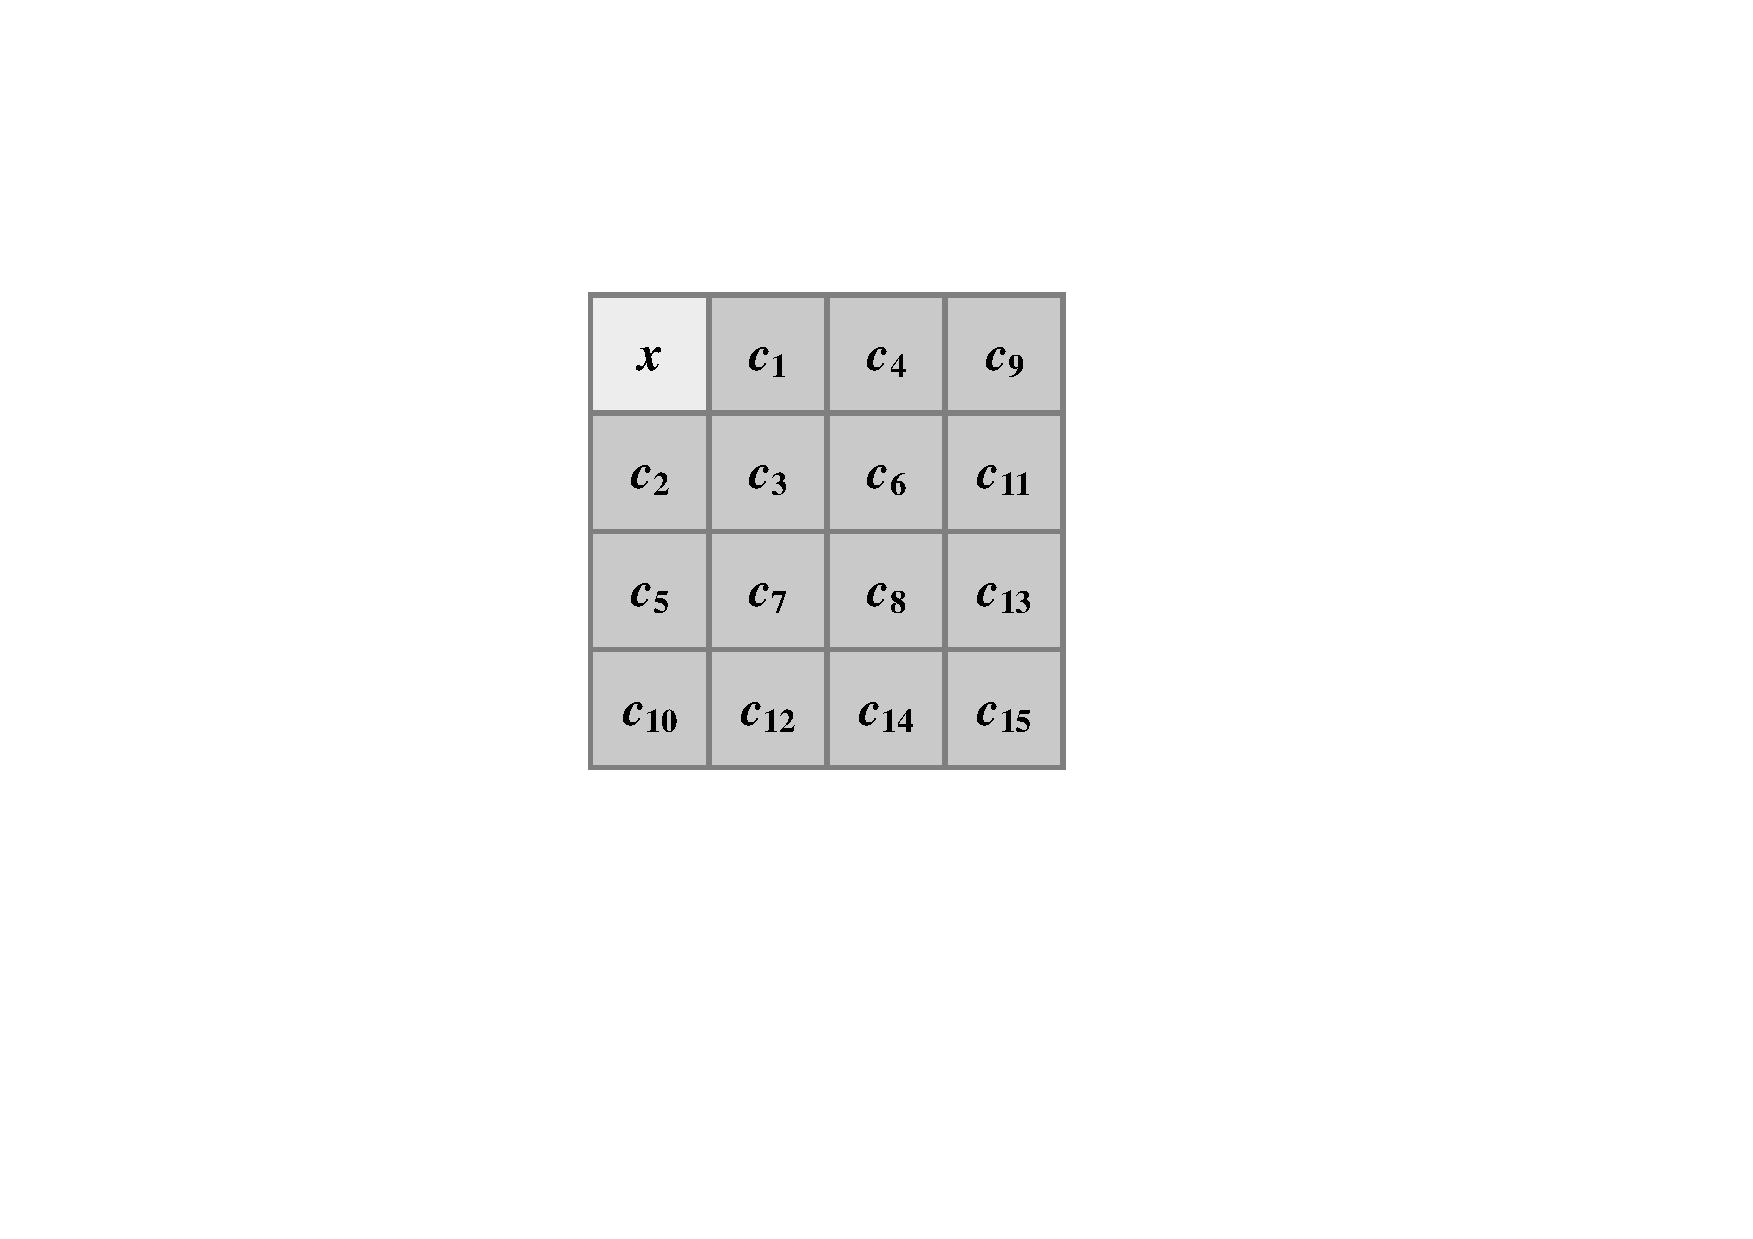
\includegraphics[width=1\textwidth]{figures/PPVOContext.pdf}
    \end{minipage}
}
\qquad\quad
\subfigure[Extended PPVO.]{
    \begin{minipage}[t]{0.37\linewidth}
    \centering
    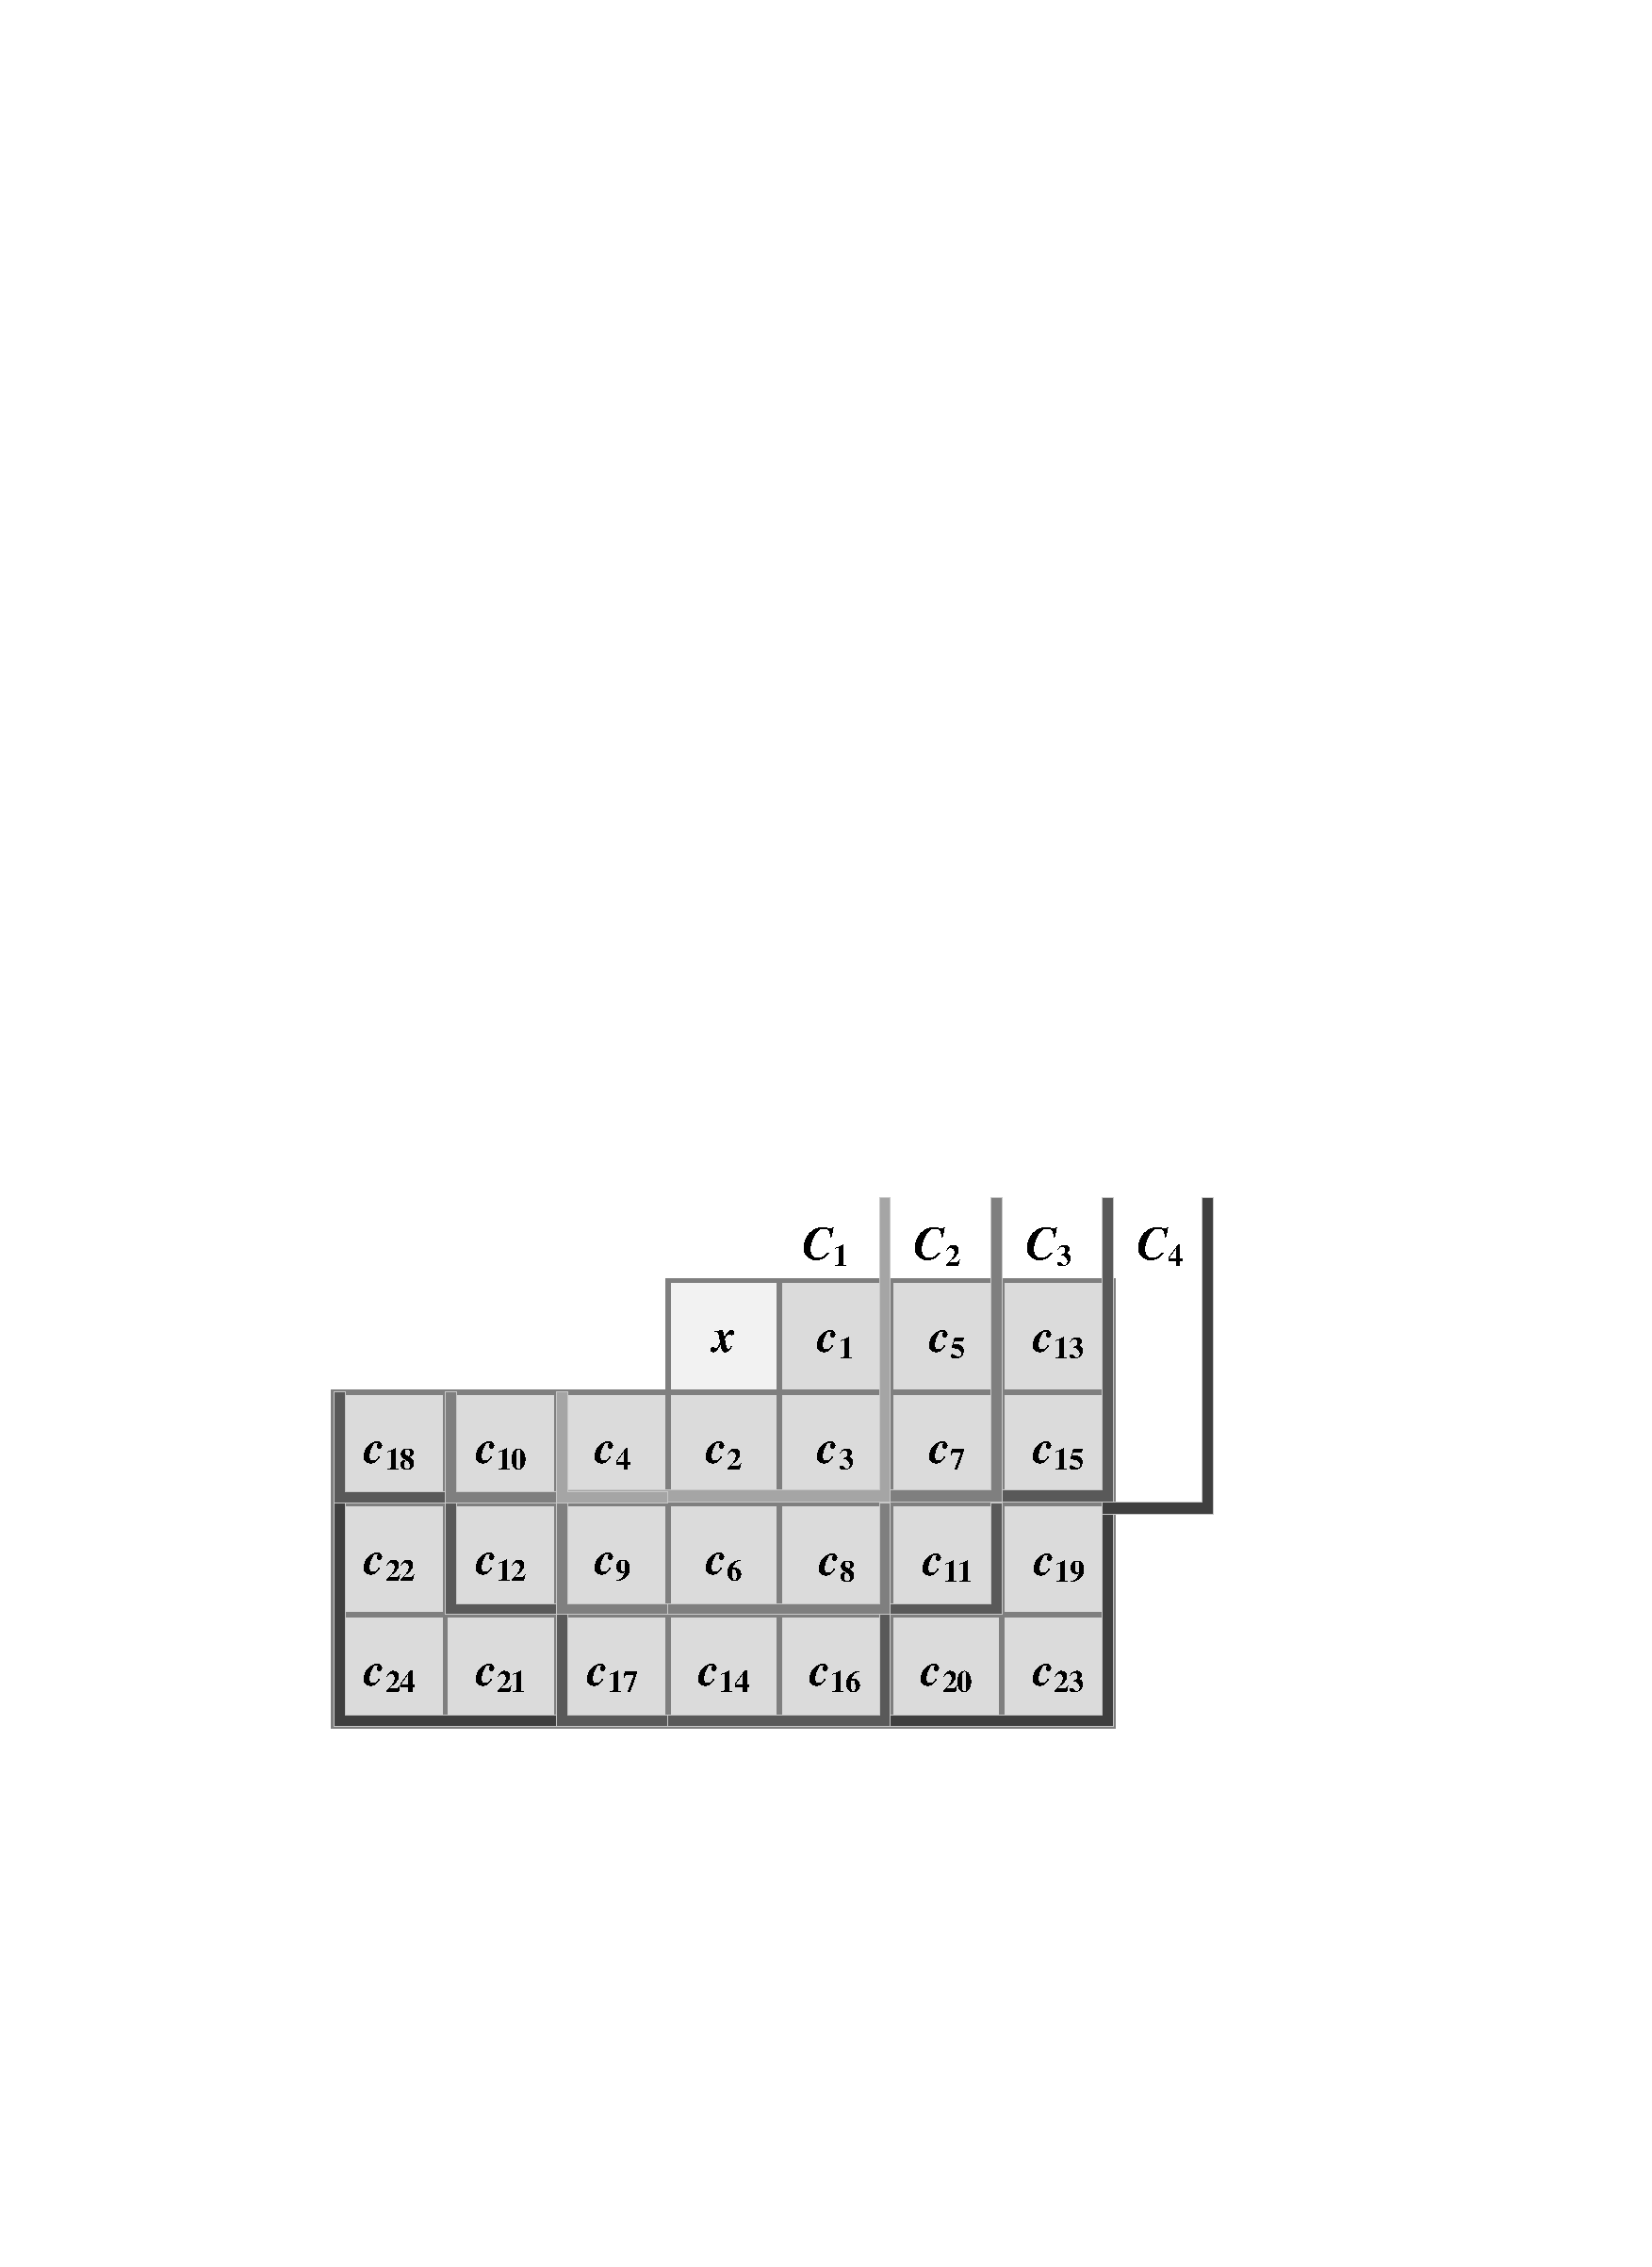
\includegraphics[width=1\textwidth]{figures/ExtendedPPVOContext.pdf}
    \end{minipage}
}		
\centering
\caption{Context pixels of PPVO(left) and Extended PPVO(right).}
\label{Fig.Context}
\end{figure*}

Here, the symbol definitions are the same as the definitions in section \ref{sec:2}. In Fig. \ref{Fig.Context}, the number of context pixels is $CN = 24$, where context pixel vector is $C = (c_{1}, ..., c_{24})$. And the prediction procedure is described as follow. Compared with PPVO, except the four sets $S_1, S_2, S_3$ and $S_4$, another set is defined as
\begin{equation*}\label{eq:S_5}
\begin{array}{ll}
S_5 = \{ x | \max(C)   =  \min(C), x > \max(C), \max(C)   \neq  254 \} \\
\end{array}.
\end{equation*}
And, for each pixel $x$, the prediction-error is calculated by
\begin{equation}\label{eq:EPPVOPE}
p = \left\{\begin{array}{ll}
x - \max(C),    & \text{if } x \in S_1  \\
\min(C) - x,    & \text{if } x \in S_2 \cup S_3 \\
0,              & \text{if } x \in S_4 \\
x - \max(C) - 1,& \text{if } x \in S_5  \\
{\rm skip},     & \text{otherwise}
\end{array}\right.,
\end{equation}
where prediction-error $p$ is located in the interval of $[0, \infty)$. By the extended PPVO predictor, with the situation of $\max(C) = \min(C)$, pixel $x$ satisfying $x > \max(C)$ is utilized to obtain prediction-errors as well. More pixels participating in prediction procedure leads to an increase in embedding capacity.

% embedding procedure
Then, as shown in Fig. \ref{Fig.ComparisonEPPVO}, bin $0$ of every PEH corresponds to the highest frequency. Considering the tradeoff between capacity and distortion, errors with the value of $0$ are utilized for data embedding. Thus, with the obtained prediction-error by (\ref{eq:EPPVOPE}), one bit data $b \in \{0, 1\}$ can be embedded by modifying $p$ to derive $\hat{p}$ by (\ref{eq:PPVOMPE}). Meanwhile, the marked pixel $\hat{x}$ can be modified by
\begin{equation}\label{eq:Embed}
\hat{x} = \left\{\begin{array}{ll}
\max(C) + \hat{p},    & \text{if } x \in S_1\\
\min(C) - \hat{p},    & \text{if } x \in S_2 \cup S_3 \\
\min(C) + \hat{p},    & \text{if } x \in S_4 \\
\max(C) + \hat{p} + 1,& \text{if } x \in S_5  \\
{\rm skip},     & \text{otherwise}
\end{array}\right..
\end{equation}

In the above embedding procedure, every prediction-error $p$ increases by $1$ or remains unchanged, i.e., $\hat{p} \geq p$.
Thus, the marked pixel value $\hat{x}$ is $1$ larger than $x$ for original pixel value of $x \in S_1 \cup S_4 \cup S_5$ and $1$ smaller than $x$ for $x \in S_2 \cup S_3$.
The pixel values after modification belong to the same collection as original pixels so that the reversibility is guaranteed for the decoder.

% show the example of histogram, comparatione and reasons.
%For extended PPVO predictor, more surrounding pixels are fully considered as pixel context to predict current pixel, aiming to get sharper histogram.
To show the superiority of extended PPVO predictor, an example is shown in Fig. \ref{Fig.ComparisonEPPVO}. In the example, comparison of normalized PEHs of extended PPVO predictor and original PPVO predictor are displayed on eight standard gray-scale $512 \times 512$ sized images. For extended PPVO predictor, eight pixels $\{c_{1}, c_{2}, c_{3}, c_{4}, c_{5}, c_{6}, c_{9}, c_{10}\}$ in Fig. \ref{Fig.Context}(b) are considered as context pixels. For a reasonable comparison, for the original PPVO predictor, eight pixels $\{c_{1}, ..., c_{8}\}$ in Fig. \ref{Fig.Context}(a) are considered as context pixels.
Obviously, normalized PEHs of extended PPVO predictor have highest peak at $0$, and the distributions are sharper, which is beneficial to the final embedding performance. Moreover, we use the embedding distortion caused by one bit data embedding to evaluate characteristic of the histogram theoretically, numerically expressed as
\begin{equation*}\label{eq:EvaluateHistogram}
{\rm \mathbf{Eval}} = \frac{{\rm H}(0)}{\frac{1}{2}{\rm H}(0)+ \sum_{i \geq 1}{\rm H}(i)},
\end{equation*}
where ${\rm H}$ is the PEH and ${\rm H}(i)$ is the frequency of pixels whose prediction-errors $p = i$. This evaluation describes the distortion caused by embedding one bit data on ${\rm H}$. The smaller the ${\rm \mathbf{Eval}}$, the better the characteristics of the PEH, which can bring less distortion. In Lena, Baboon and Airplane, ${\rm \mathbf{Eval}}$ of extended PPVO predictor are 2.07, 6.88 and 1.44 respectively, while value of evaluation are 2.81, 7.90 and 1.76 of PPVO predictor. This indicates that data embedding on PEH of extended PPVO predictor may carry much less distortion to obtain the better performance.
\begin{figure*}
\centering
\subfigure[Lena]{
    \begin{minipage}[t]{0.225\linewidth}
    \centering
    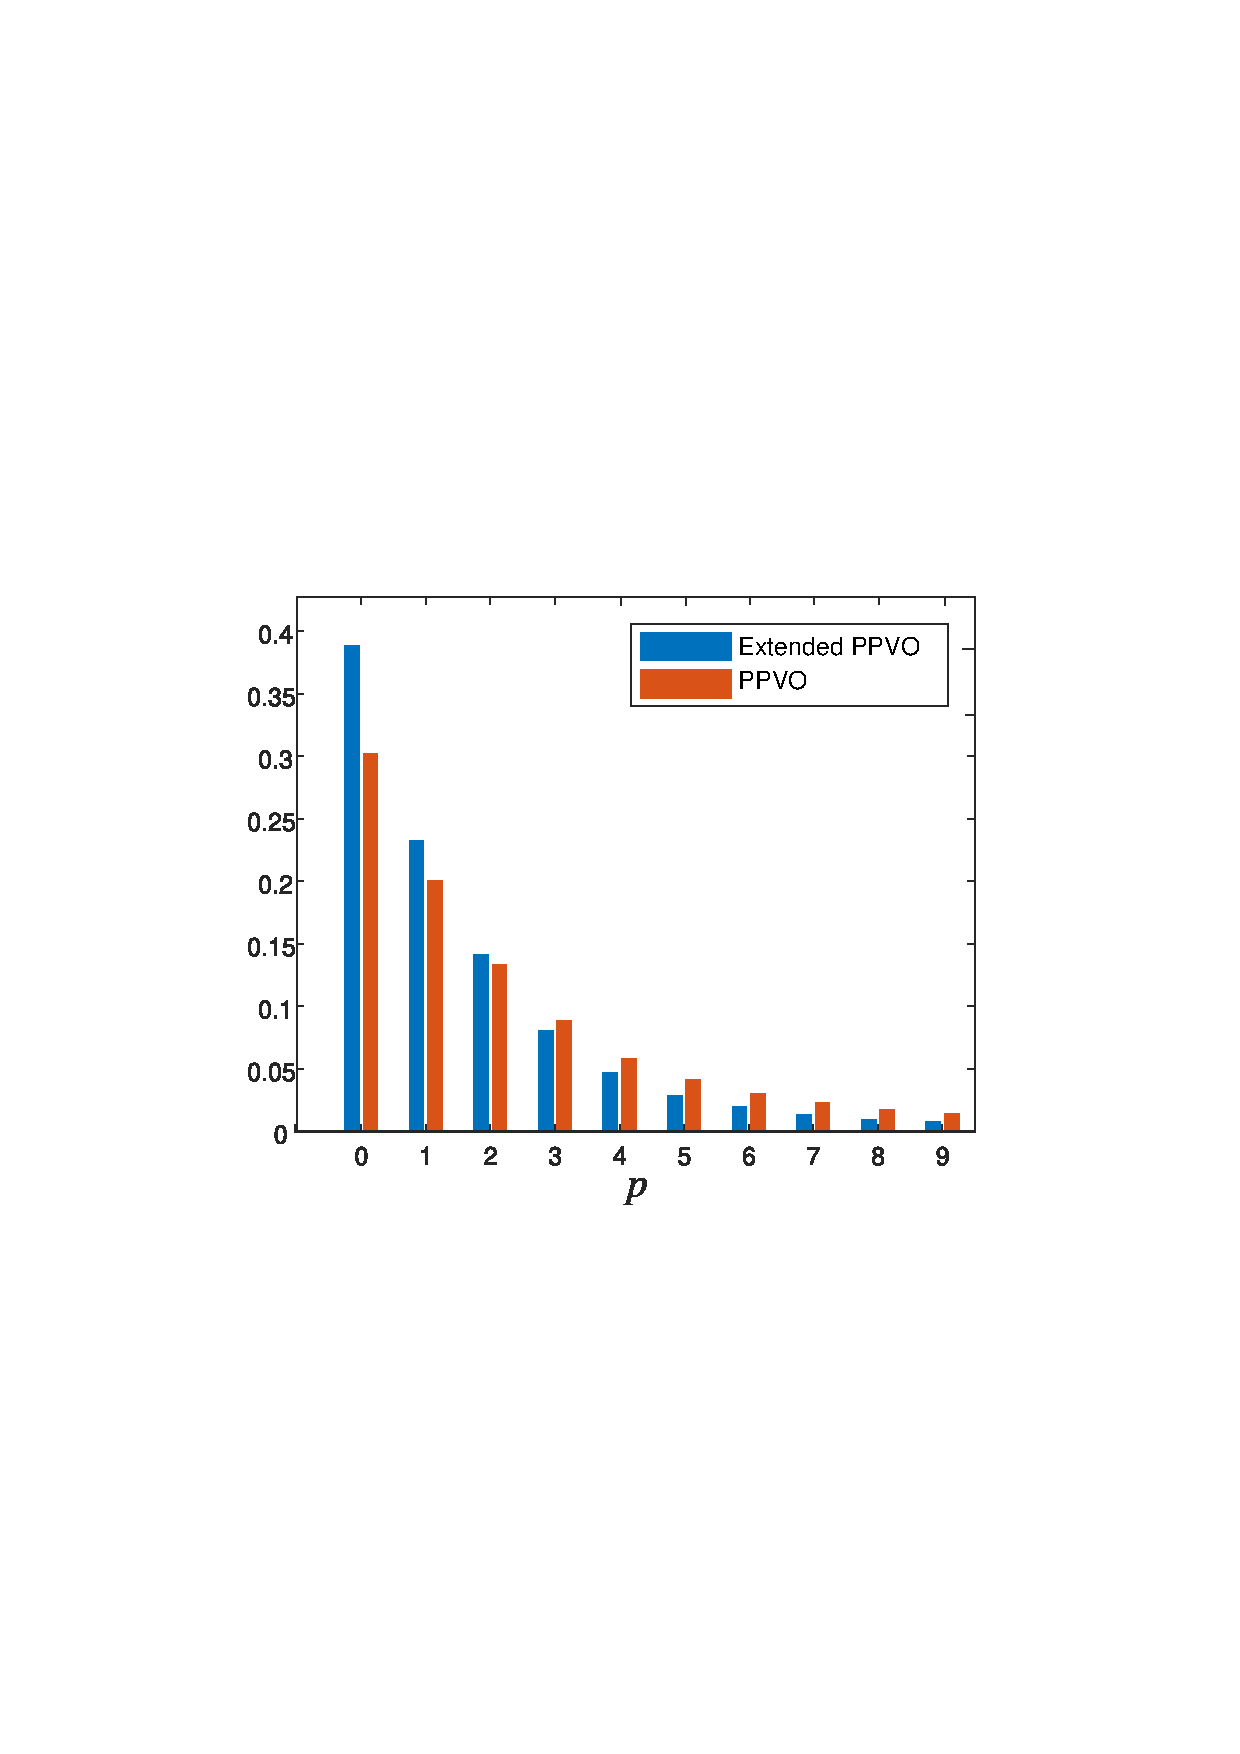
\includegraphics[width=1\textwidth]{figures/Comparison/lena.pdf}
    \end{minipage}
}
\subfigure[Baboon]{
    \begin{minipage}[t]{0.225\linewidth}
    \centering
    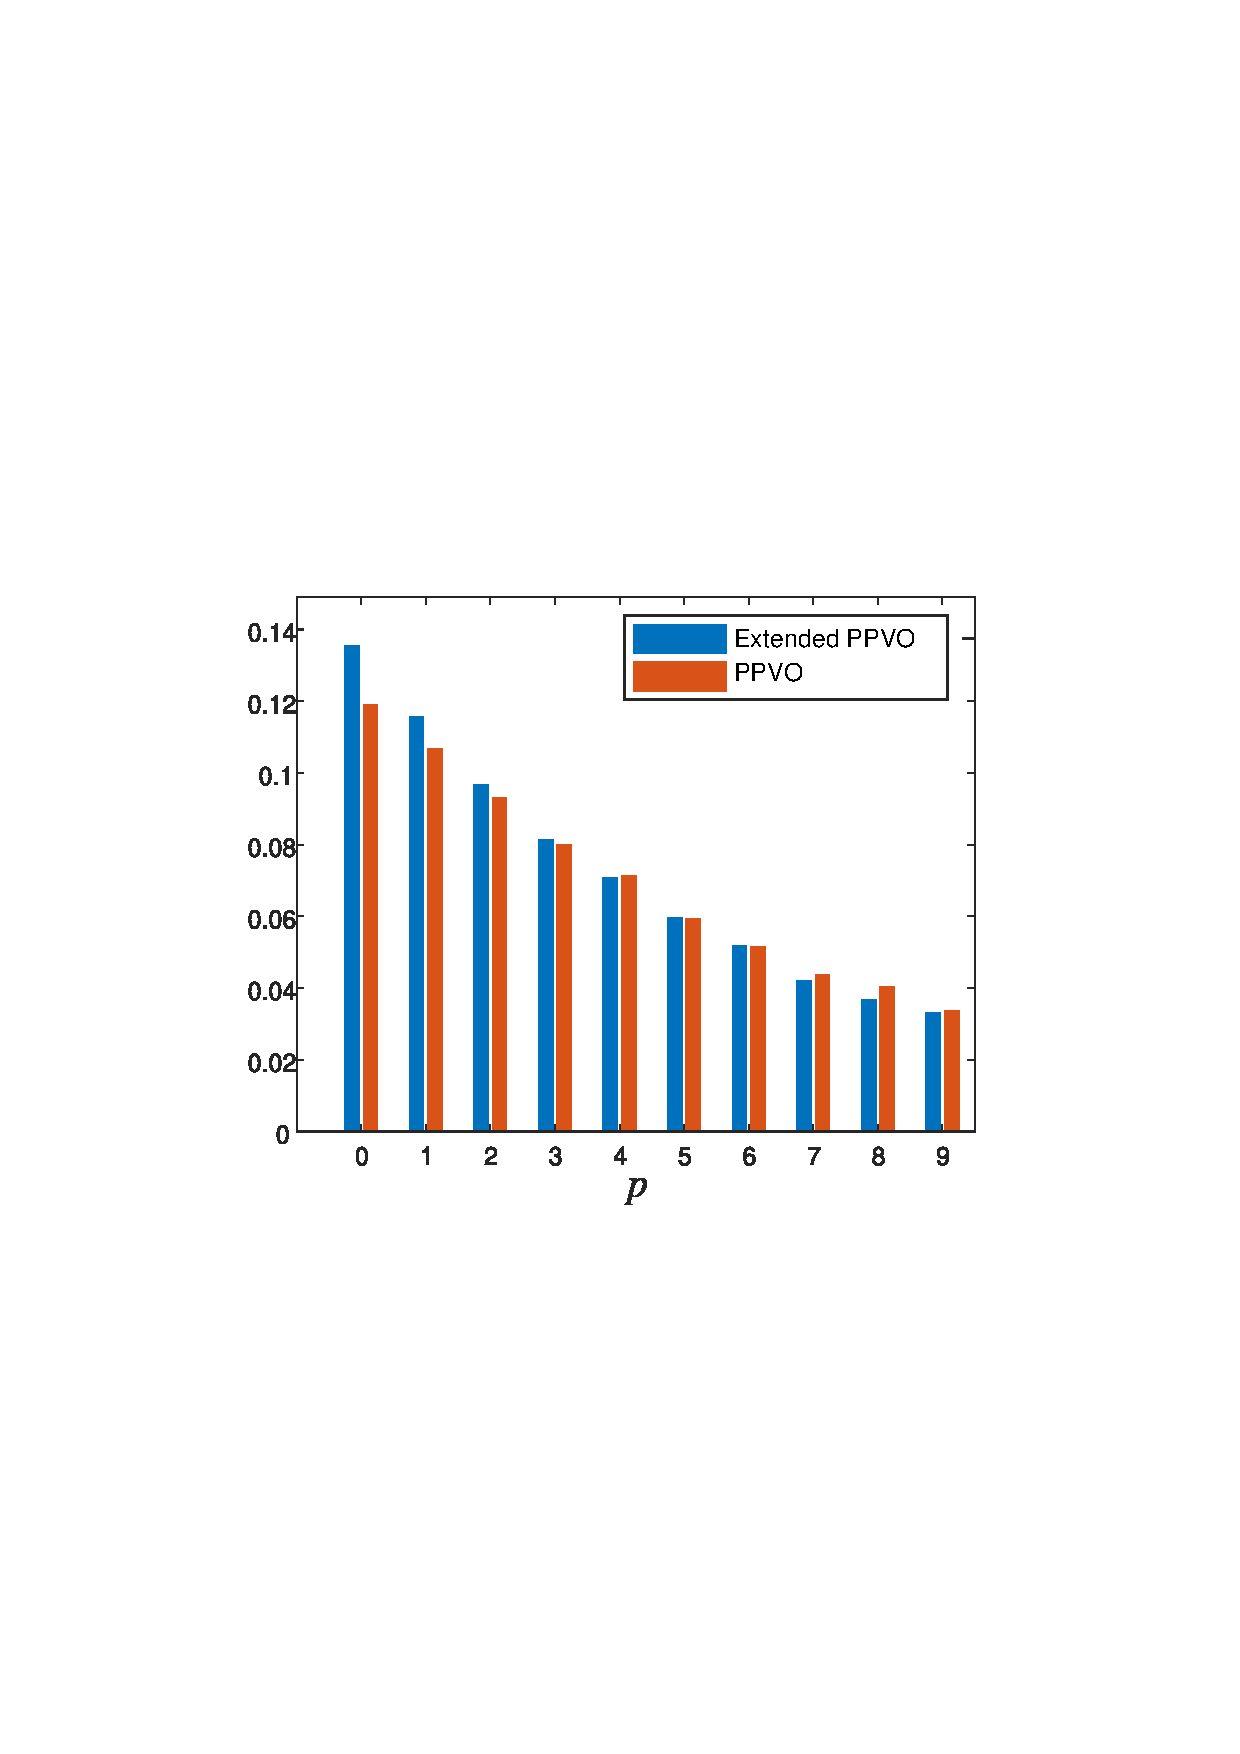
\includegraphics[width=1\textwidth]{figures/Comparison/baboon.pdf}
    \end{minipage}
}
\subfigure[Airplane]{
    \begin{minipage}[t]{0.225\linewidth}
    \centering
    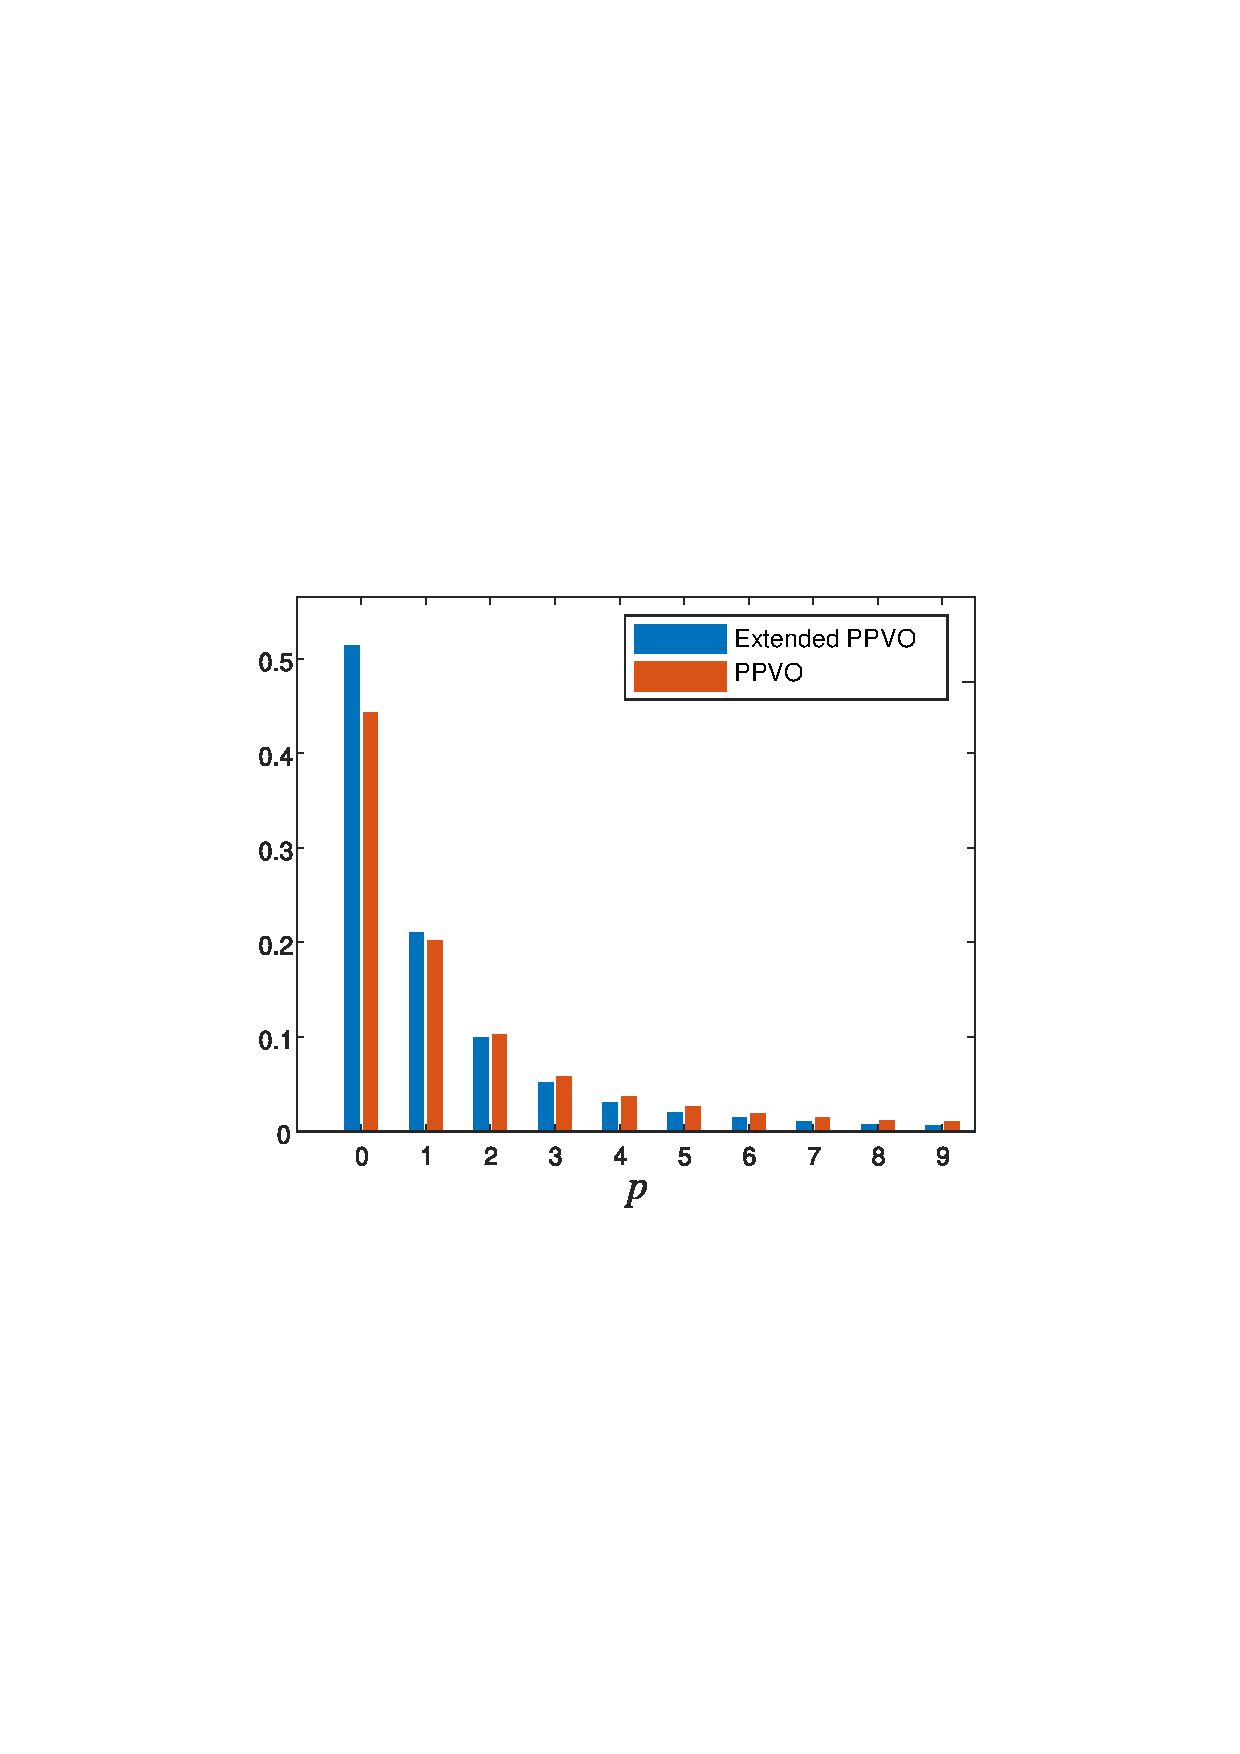
\includegraphics[width=1\textwidth]{figures/Comparison/airplane.pdf}
    \end{minipage}
}
\subfigure[Barbara]{
    \begin{minipage}[t]{0.225\linewidth}
    \centering
    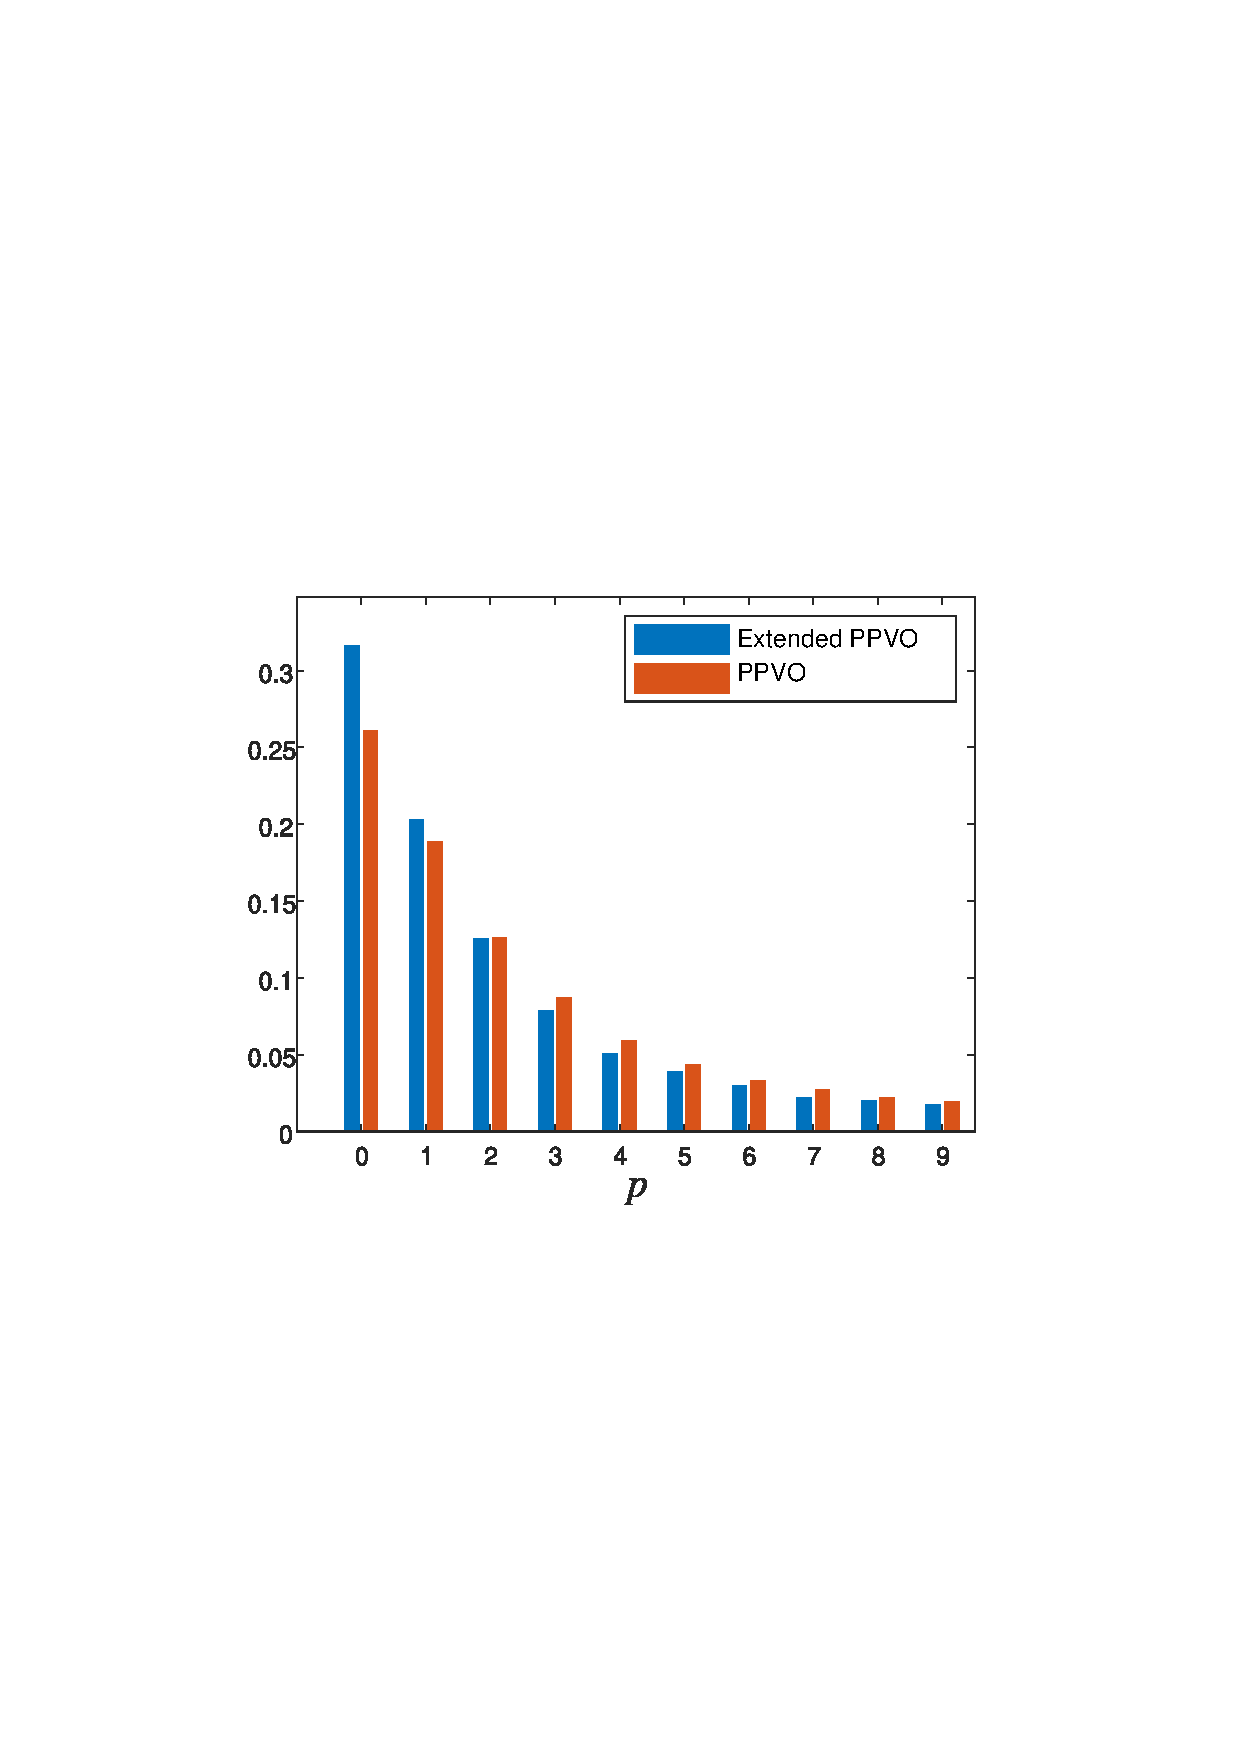
\includegraphics[width=1\textwidth]{figures/Comparison/barbara.pdf}
    \end{minipage}
}


\subfigure[Lake]{
    \begin{minipage}[t]{0.225\linewidth}
    \centering
    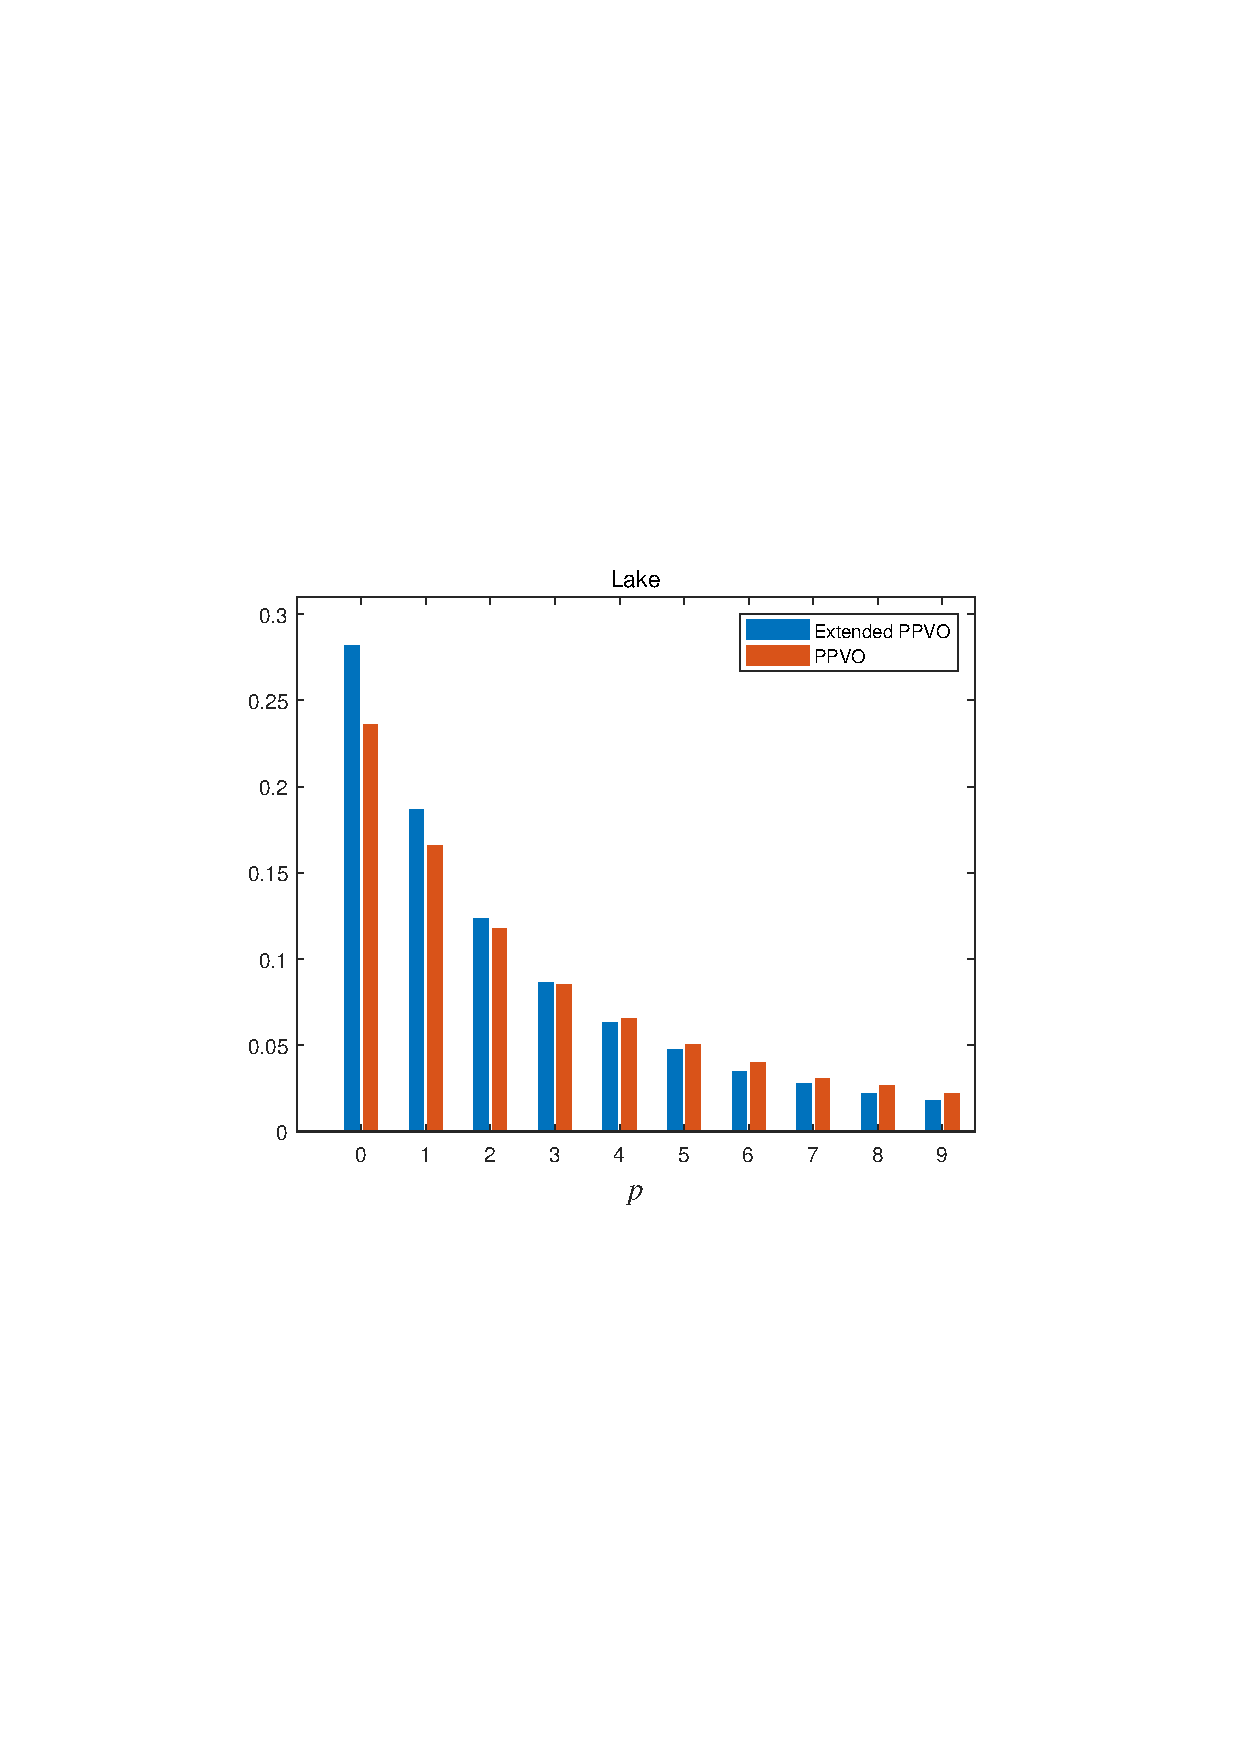
\includegraphics[width=1\textwidth]{figures/Comparison/lake.pdf}
    \end{minipage}
}
\subfigure[Peppers]{
    \begin{minipage}[t]{0.225\linewidth}
    \centering
    \includegraphics[width=1\textwidth]{figures/Comparison/peppers.pdf}
    \end{minipage}
}
\subfigure[Boat]{
    \begin{minipage}[t]{0.225\linewidth}
    \centering
    \includegraphics[width=1\textwidth]{figures/Comparison/boat.pdf}
    \end{minipage}
}
\subfigure[Eliane]{
    \begin{minipage}[t]{0.225\linewidth}
    \centering
    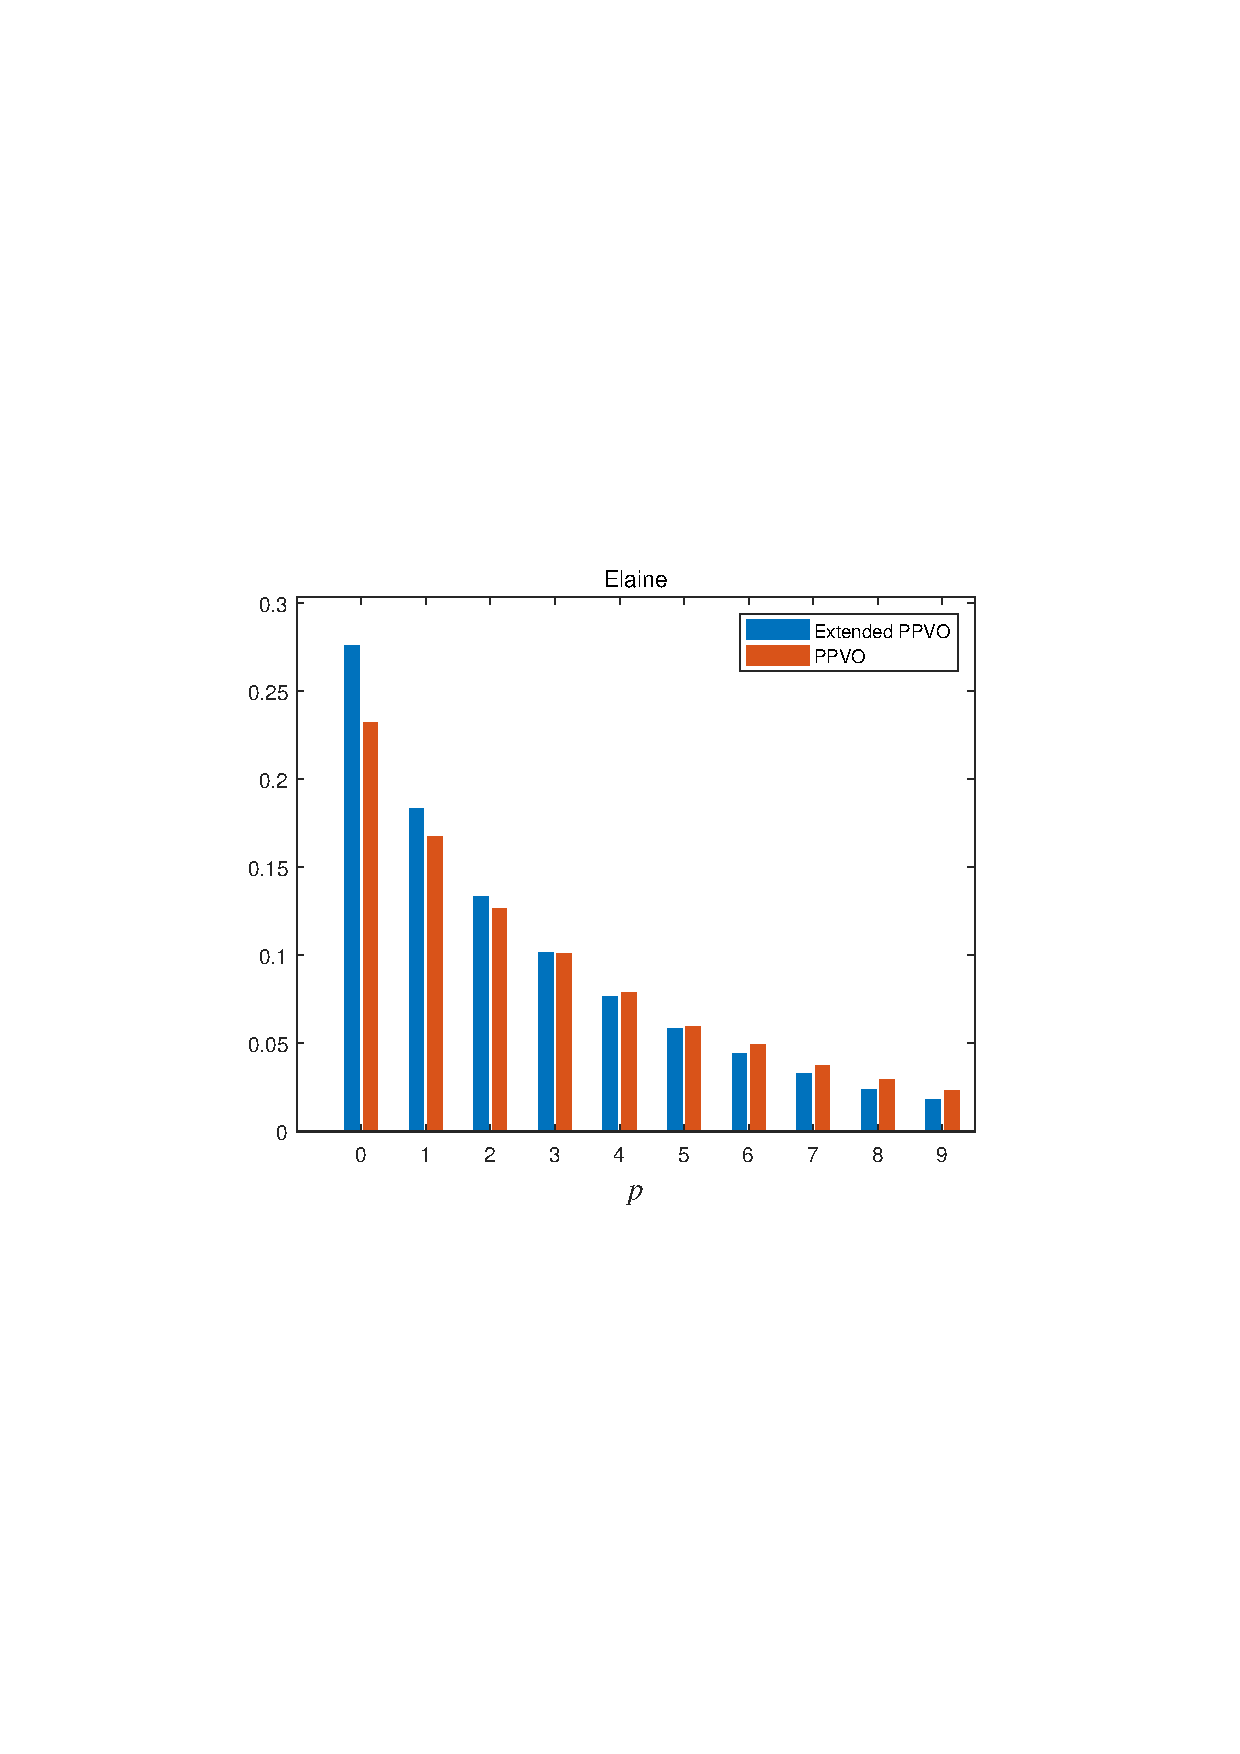
\includegraphics[width=1\textwidth]{figures/Comparison/elaine.pdf}
    \end{minipage}
}
\centering
\caption{Comparison of normalized prediction-errors $p$ of extended PPVO by (\ref{eq:EPPVOPE}) in blue and PPVO by (\ref{eq:PPVOPE}) in orange.}
\label{Fig.ComparisonEPPVO}
\end{figure*}


\subsection{Multi-size based Embedding Method for MHM}\label{sec:3.2}
In above embedding procedure, ${\rm CN}$ of $x$ to be predicted is already set in advance. And for a cover image, every pixel is predicted by the same region of context pixels. Actually, the performance results caused by different context pixels are different. In order to explore the impact of ${\rm CN}$, we consider ${\rm CN} \leq 24$ and, to simplify the presentations, context pixels are group into four sets according to size of the region around the current pixel $x$, including $C_1 = \{c_1, ..., c_4\}$, $C_2 = \{c_1, ..., c_{10}\}$, $C_3 = \{c_1, ..., c_{18}\}$ and $C_4 = \{c_1, ..., c_{24}\}$, as shown in Fig. \ref{Fig.Context}(b). It is expected that the distortions are different by using different size context regions for prediction as shown in Fig. \ref{Fig.Eval}(a). In addition, Based on the consideration of the complexity of traditional RDH embedding, the comparison of threshold-capacity curves and threshold-${\rm \mathbf{Eval}}$ curves are shown in Fig. \ref{Fig.Eval}(b) and Fig. \ref{Fig.Eval}(c) as well. Here a threshold $T$ is set to choose
the smooth pixels whose complexity ${\rm NL} < T$ to generate PEH so that all secret data can just be embedded. And the complexity of one pixel is evaluated by the sum of the absolution differences of the horizontal and vertical of every two adjacent pixels belong to the corresponding context.

In Fig. \ref{Fig.Eval}, we focus on the two curves of $C_1$ and $C_2$. According to the curves, there are a few observations as follows.
\begin{enumerate}
  \item In Fig. \ref{Fig.Eval}(b), the maximum embedding capacity of $C_1$ is much larger than $C_2$. This is because almost pixels in the cover image with small ${\rm CN}$ is used to be predicted while part of the pixels are skipped with larger size $C_2$.
  \item In Fig. \ref{Fig.Eval}(b), capacity increases very fast when the threshold $T$ increases from a small value, especially curve of $C_1$. This indicates that pixels at smooth region are more suitable to be predicted.
  \item In Fig. \ref{Fig.Eval}(c), With the same threshold $T$, although the capacity of $C_2$ is smaller than $C_1$, ${\rm \mathbf{Eval}}$ of $C_2$ is much smaller than $C_1$. This observation illustrates that among the skipped pixels of $C_2$, the proportion of pixels that are predicted to be inaccurate is increase, which is no benefit to the performance.
\end{enumerate}
Through the above description, it shows that prediction with context pixels in smaller size achieves a large embedding capacity, but distortion also increases due to the pixels to be predicted inaccurately. And for the pixels in larger size, lots of inaccurately predicted pixels are skipped and distortion is much less than the smaller size. But the embedding capacity is limited. Based on these consideration, there mush be a strategy to combine the advantages of both size context to further improve embedding performance.
%we propose a scheme called a multi-size based embedding method for MHM, which combines the advantages of both size context to further improve embedding performance.

Here an example is taken to bring out the strategy. As shown in Fig. \ref{Fig.Eval}(a), some thresholds are marked on the curves of $C_1$ and $C_2$. Specifically, we let $X_{T} = \{x |\ {\rm NL}(x) < T\}$. $X_{T}$ indicates the set of pixels with complexity less than $T$. The ${\rm \mathbf{Eval}}$ of $X_{72}$ with $C_1$ is $1.34$, which is approximately equal to the $X_{94}$ with $C_2$. The ${\rm \mathbf{Eval}}$ of the $X_{94}$ with $C_1$ equals 1.59 and it is much larger than $1.34$. It means that pixels in $X_{94} \setminus X_{72} = \{x|\ 72 \leq {\rm NL}(x) < 94\}$ with $C_1$ for prediction bring much more distortion than $C_2$. In other words, it will effectively reduce the distortion if pixels $x \in X_{72}$ are predicted by the context pixels with $C_1$ and pixels $x \in X_{94} \setminus X_{72}$ are predicted by the context pixels with $C_2$. The similar conclusion can be obtained on sets $X_{122}$ and $X_{277} \setminus X_{122}$. Thus, a detailed description of the multi-size based embedding method is given.
\begin{figure*}
\centering
\subfigure[]{
    \begin{minipage}[t]{0.3\linewidth}
    \centering
    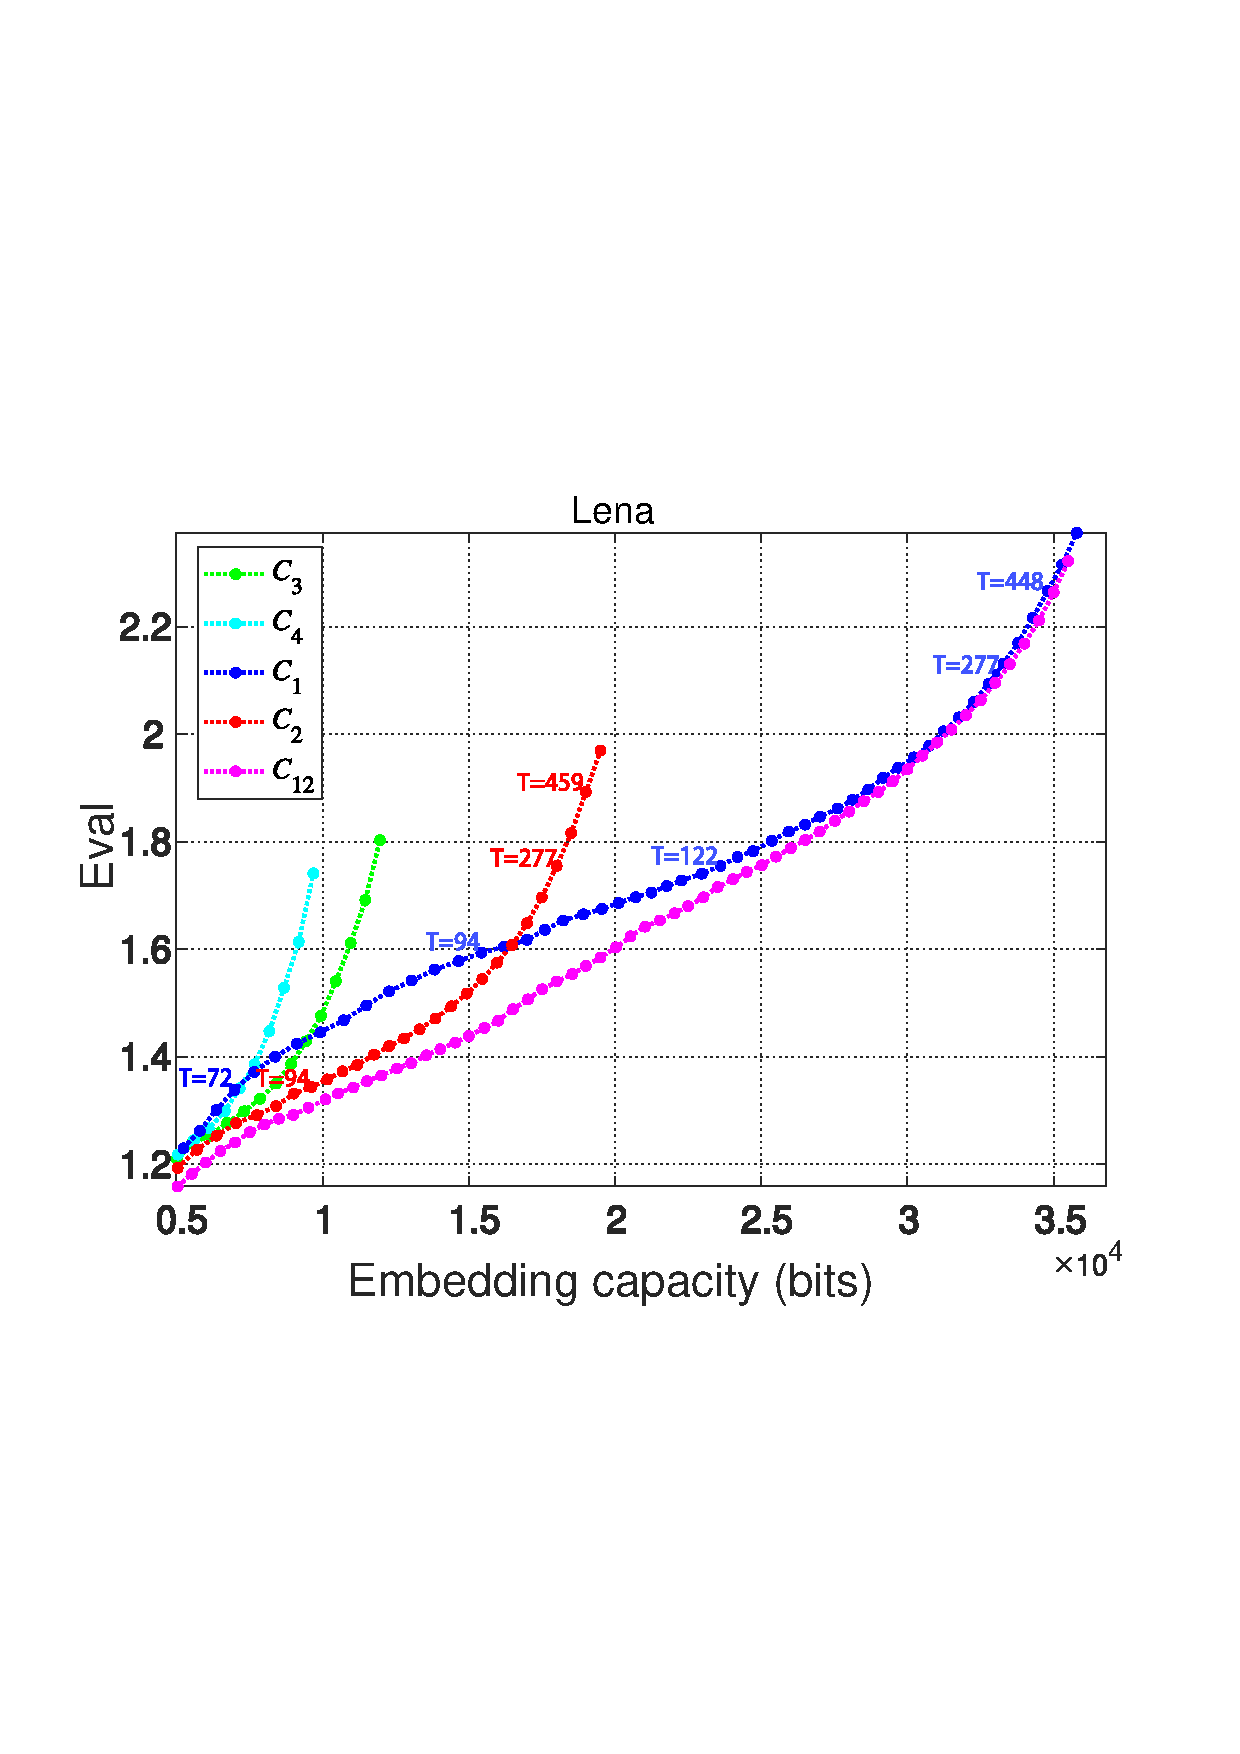
\includegraphics[width=1\textwidth]{figures/EvalLena.pdf}
    \end{minipage}
}
\subfigure[]{
    \begin{minipage}[t]{0.31\linewidth}
    \centering
    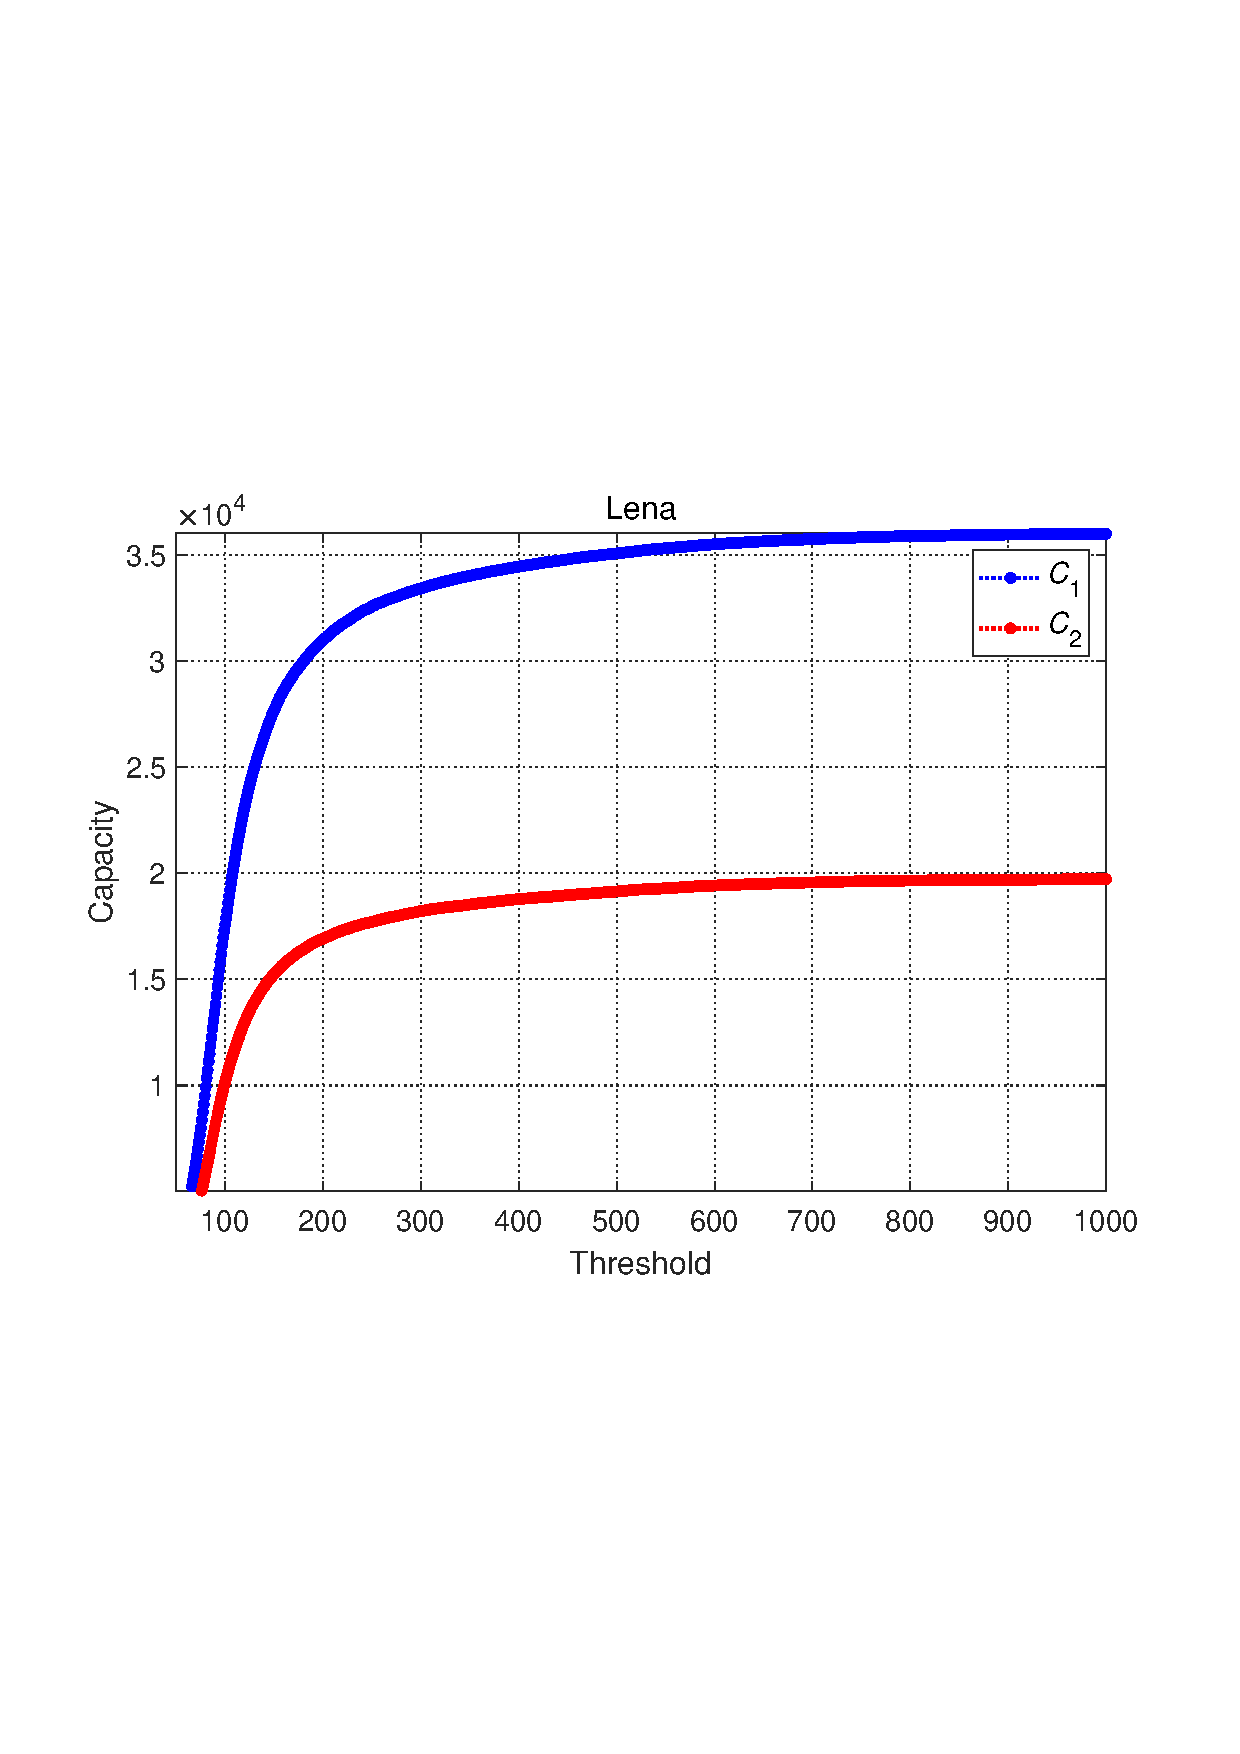
\includegraphics[width=1\textwidth]{figures/CapLena.pdf}
    \end{minipage}
}
\subfigure[]{
    \begin{minipage}[t]{0.31\linewidth}
    \centering
    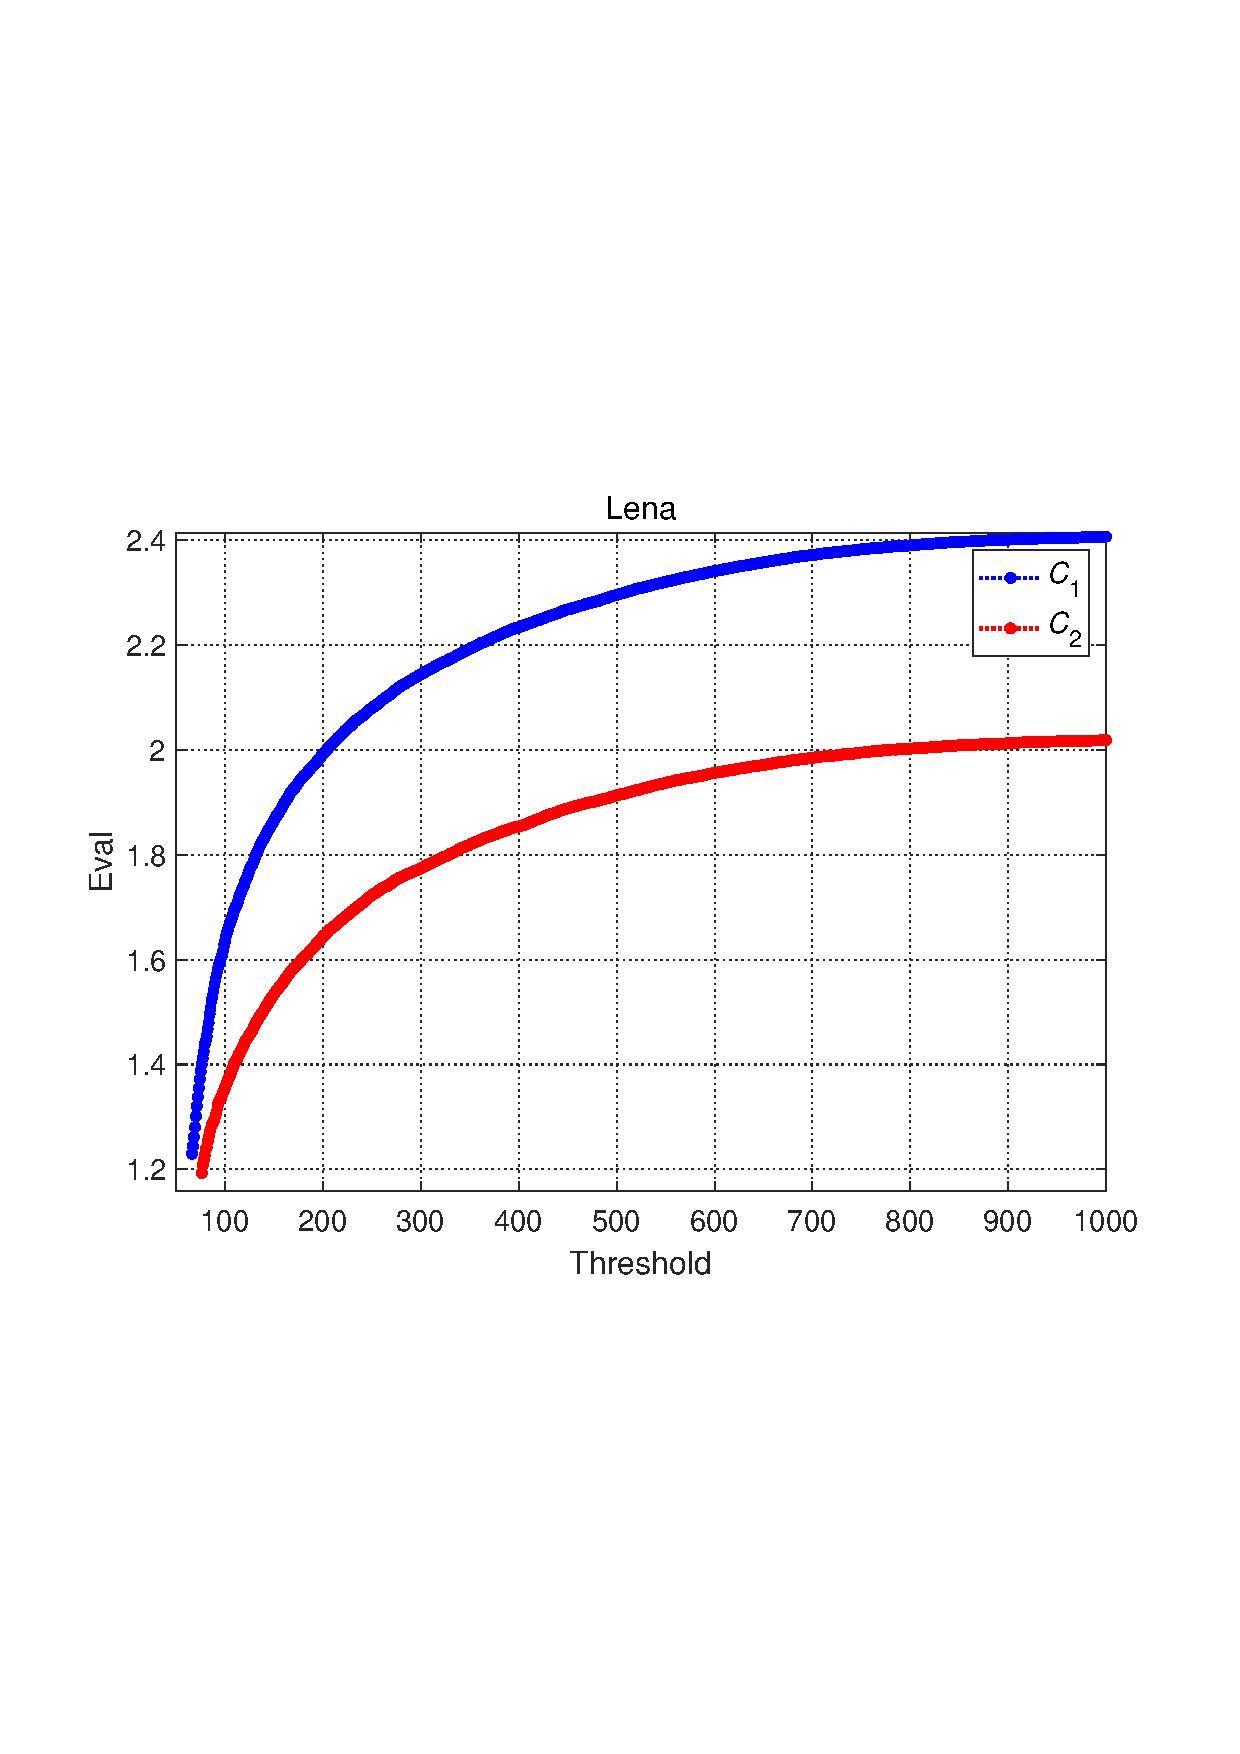
\includegraphics[width=1\textwidth]{figures/thEvalLena.pdf}
    \end{minipage}
}
\centering
\caption{Eval.}
\label{Fig.Eval}
\end{figure*}

%% embedding method
In the proposed method, to utilize the two size of $C_1$ and $C_2$ for prediction, pixels on the cover images are divided into three parts by two thresholds $T_1$, $T_2$ ($0 \leq T_1 \leq T2$). The context of pixels of $X_{T_1}$ are seen as smooth region, and these pixels are predicted by the context pixels of $C_1$. Pixels in $X_{T_2} \setminus X_{T_1}$ are predicted by the context pixels of $C_2$, and other pixels are all omitted. The above strategy is reasonable. In Fig. \ref{Fig.Eval}(c), it shows that the distance between the two curves is growing with the increase of threshold. This verify that in the area with higher complexity, more inaccurately predicted pixels are skipped with context pixels in $C_2$. Therefore, the pixels in smooth regions $X_{T_1}$ is predicted by the context pixels of $C_1$. This provides much more embedding capacity. And for the pixels in the normal regions $X_{T_2}$, pixels of $C_2$ are chosen as context pixels to predict, making the distortion as low as possible. For example, Fig. \ref{Fig.EmbedExample} shows the the embedding procedures for the three types of pixels, where $(T_1, T_2) = (15, 25)$. For the first pixel value $x = 150$, because the complexity ${\rm NL} = 10$ of the pixel less than the small threshold $T_1$, the pixel is in a smooth region and context pixels $C = \{148, 150, 150, 148\}$ are chosen. The prediction-error of the pixel value is $p = 0$. One bit secret data $b = 1$ can be embedded by increasing the $x$ by $1$ to $\hat{x} = 151$. However, if context pixels of $C_2$ are chosen for prediction, the pixel wound be skipped because of $\min(C) < x < \max(C)$. For the second pixel $x = 135$, it is in normal region, where the complexity value ${\rm NL} = 24$ larger than $T_1$ but less than $T_2$. The context pixels $C = \{137, 136, 139, 138, 140, 135, 142, 137, 136, 139\}$ are chosen and prediction-error is $p = 0$. One bit data $b = 0$ can be embedded by remaining the pixel value $\hat{x} = x = 135$. If context pixels of $C_1$ are chosen, the prediction-error wound be $p = 1$ and no one bit data wound be embedded. The Third pixel $x = 147$ is in the rough region whose complexity ${\rm NL} = 34$ larger than $T_2$ and it is skipped.
\begin{figure*}
\centering
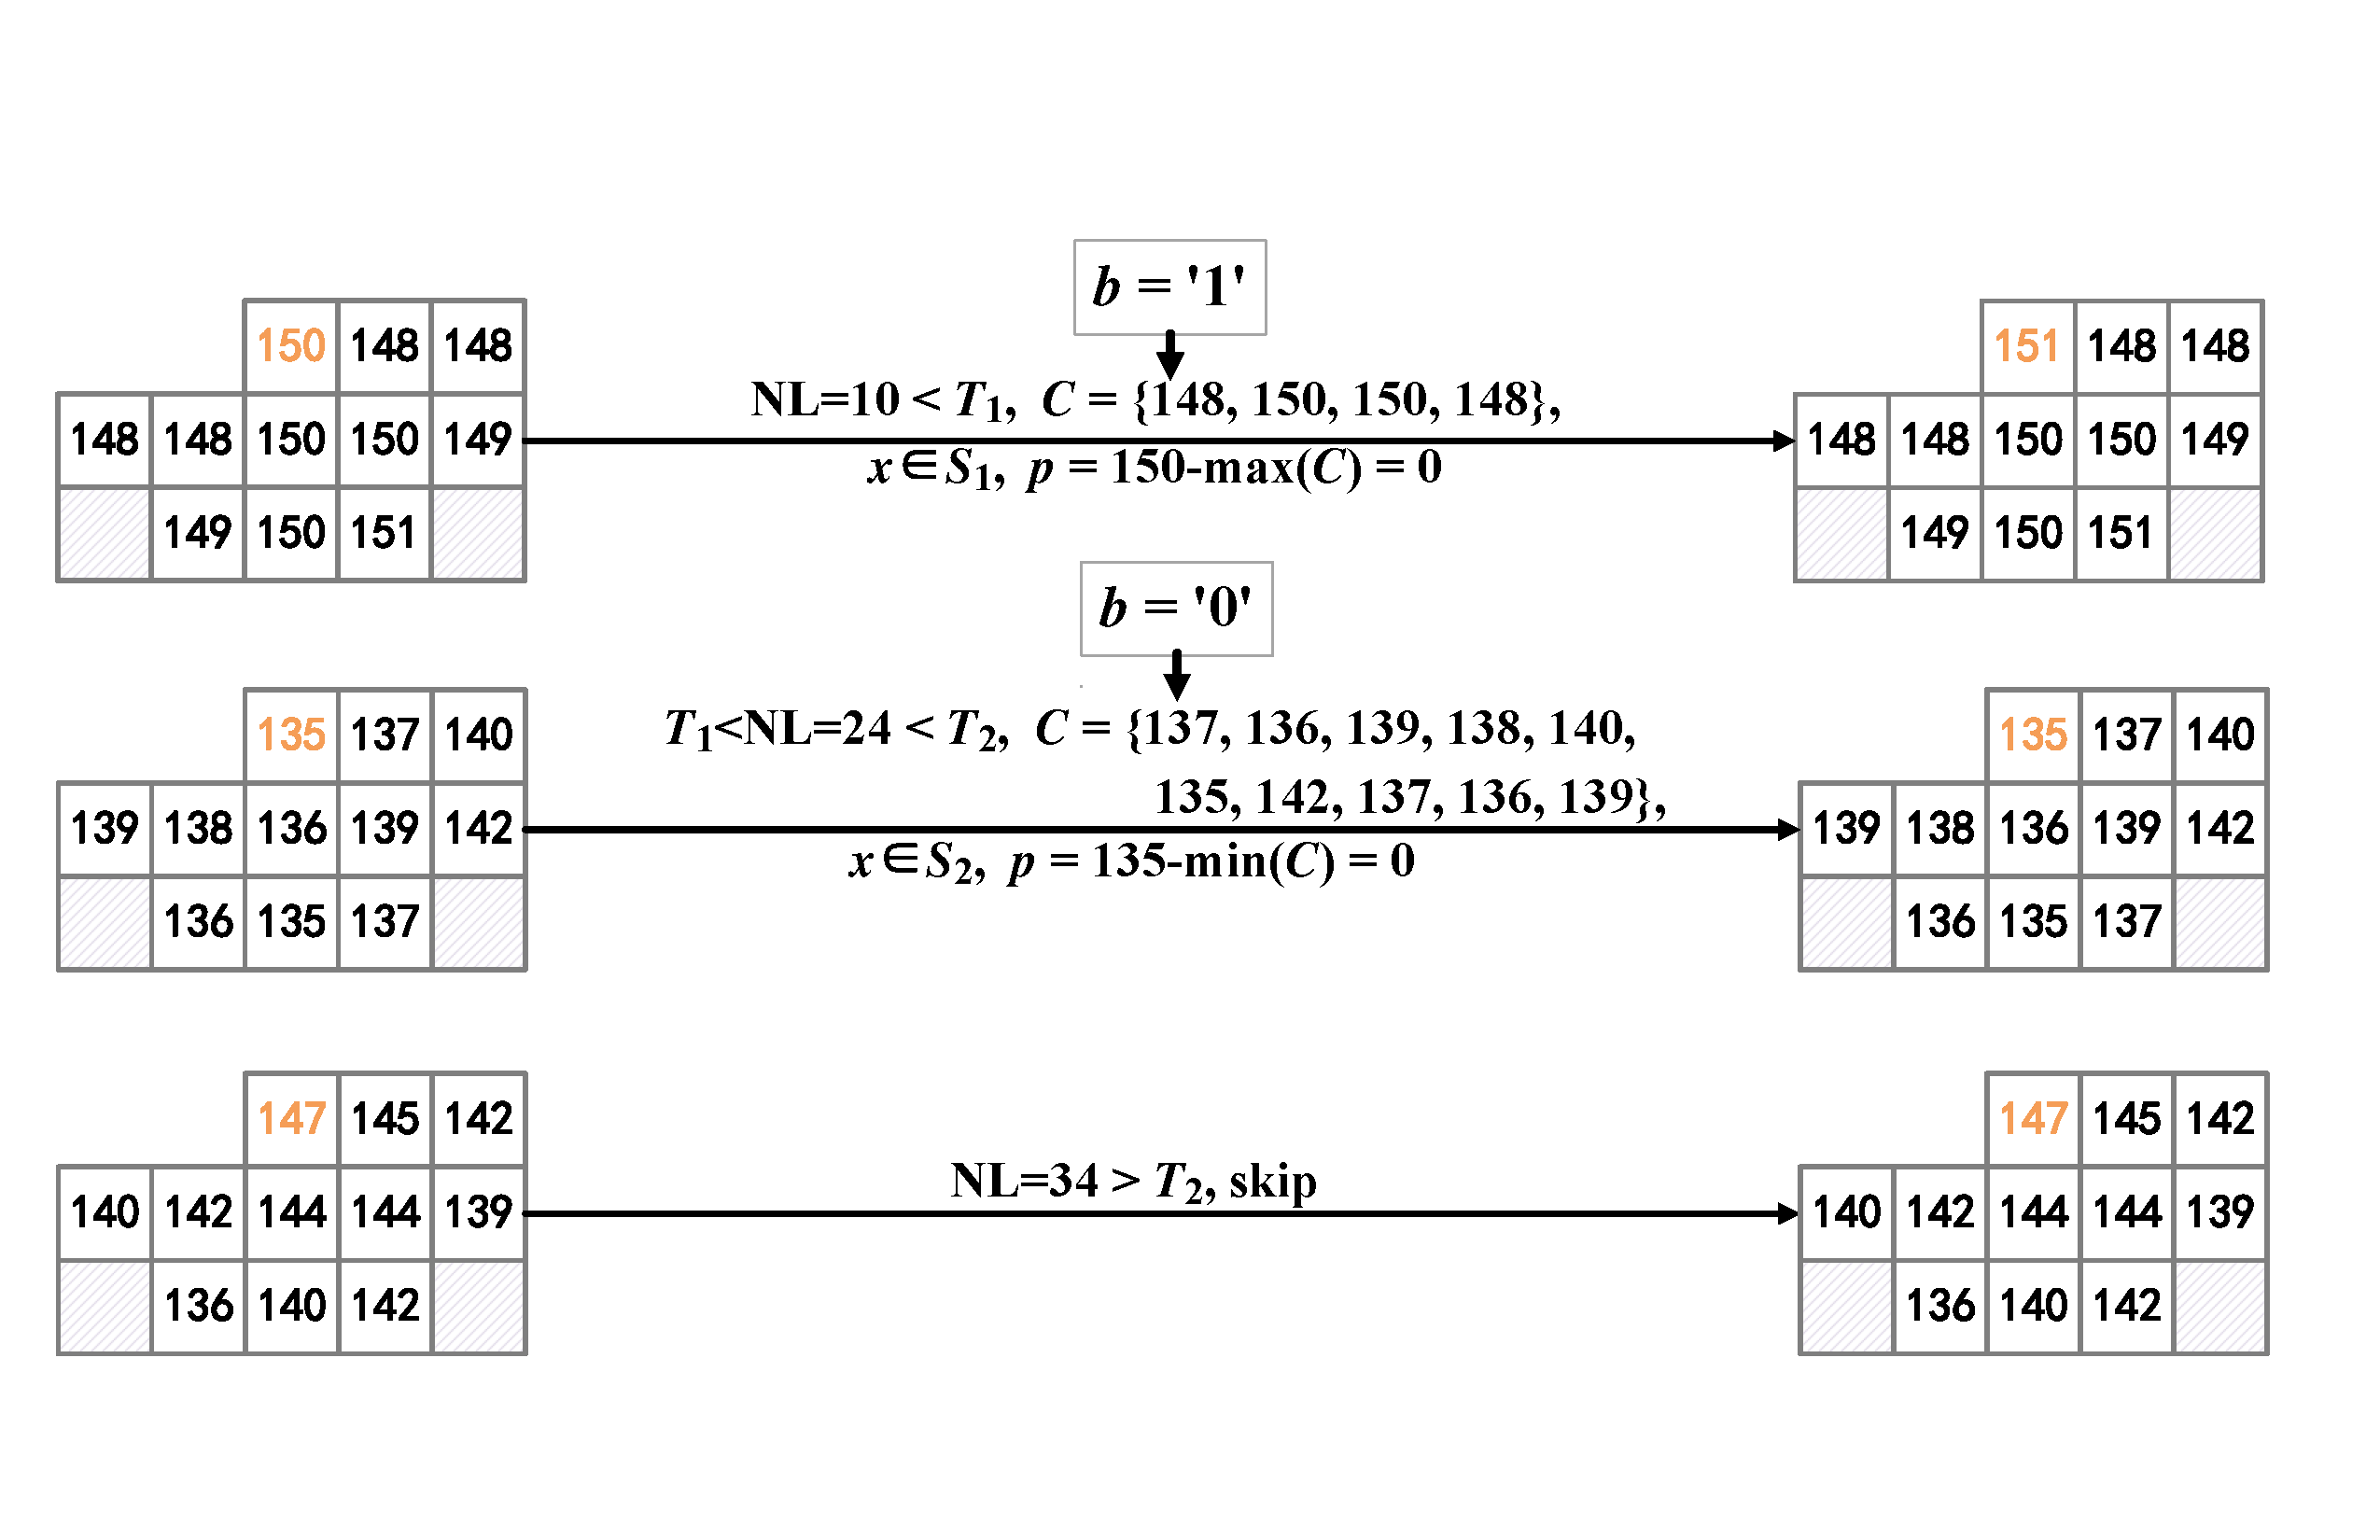
\includegraphics[width=0.85\textwidth]{figures/EmbedwithTh.pdf}
\centering
\caption{Example.}
\label{Fig.EmbedExample}
\end{figure*}

And for the purpose of finding suitable thresholds, let ${\rm H}_{(T_1, T_2)}$ as the histogram of prediction-errors derived from the pixels in $X_{T_1}$ with $C_1$ and pixels in $X_{T2} \setminus X_{T_2}$ with $C_2$. For a given embedding capacity $EC$, the optimal thresholds $(T_1^*, T_2^*)$ are obtained by
\begin{equation}\label{eq:thresholds}
\begin{array}{ll}
\mathop{\arg\min}\limits_{0 \leq T_1 \leq T_2} & \frac{\frac{1}{2}{\rm H}_{(T_1, T_2)}(0) + \sum_{i \geq 1}{\rm H}_{(T_1, T_2)}(i)}{{\rm H}_{(T_1, T_2)}(0)}\\
s.t.                                    & {\rm H}_{(T_1, T_2)}(0) \geq EC
\end{array}.
\end{equation}
Fig. \ref{Fig.Thresholds} shows the optimal thresholds $(T_1^*, T_2^*)$ by (\ref{eq:thresholds}) for some capacities. It is note that the two optimal thresholds are positively correlated. However, it is difficult to find the exact relationship between them. So, in the optimization process, we find the optimal parameters by traversing all the values. The pink curve of $C_{12}$ in Fig. \ref{Fig.Context}(a) shows the better result is achieved by combining two size context with two complexity thresholds.
\begin{figure*}
\centering
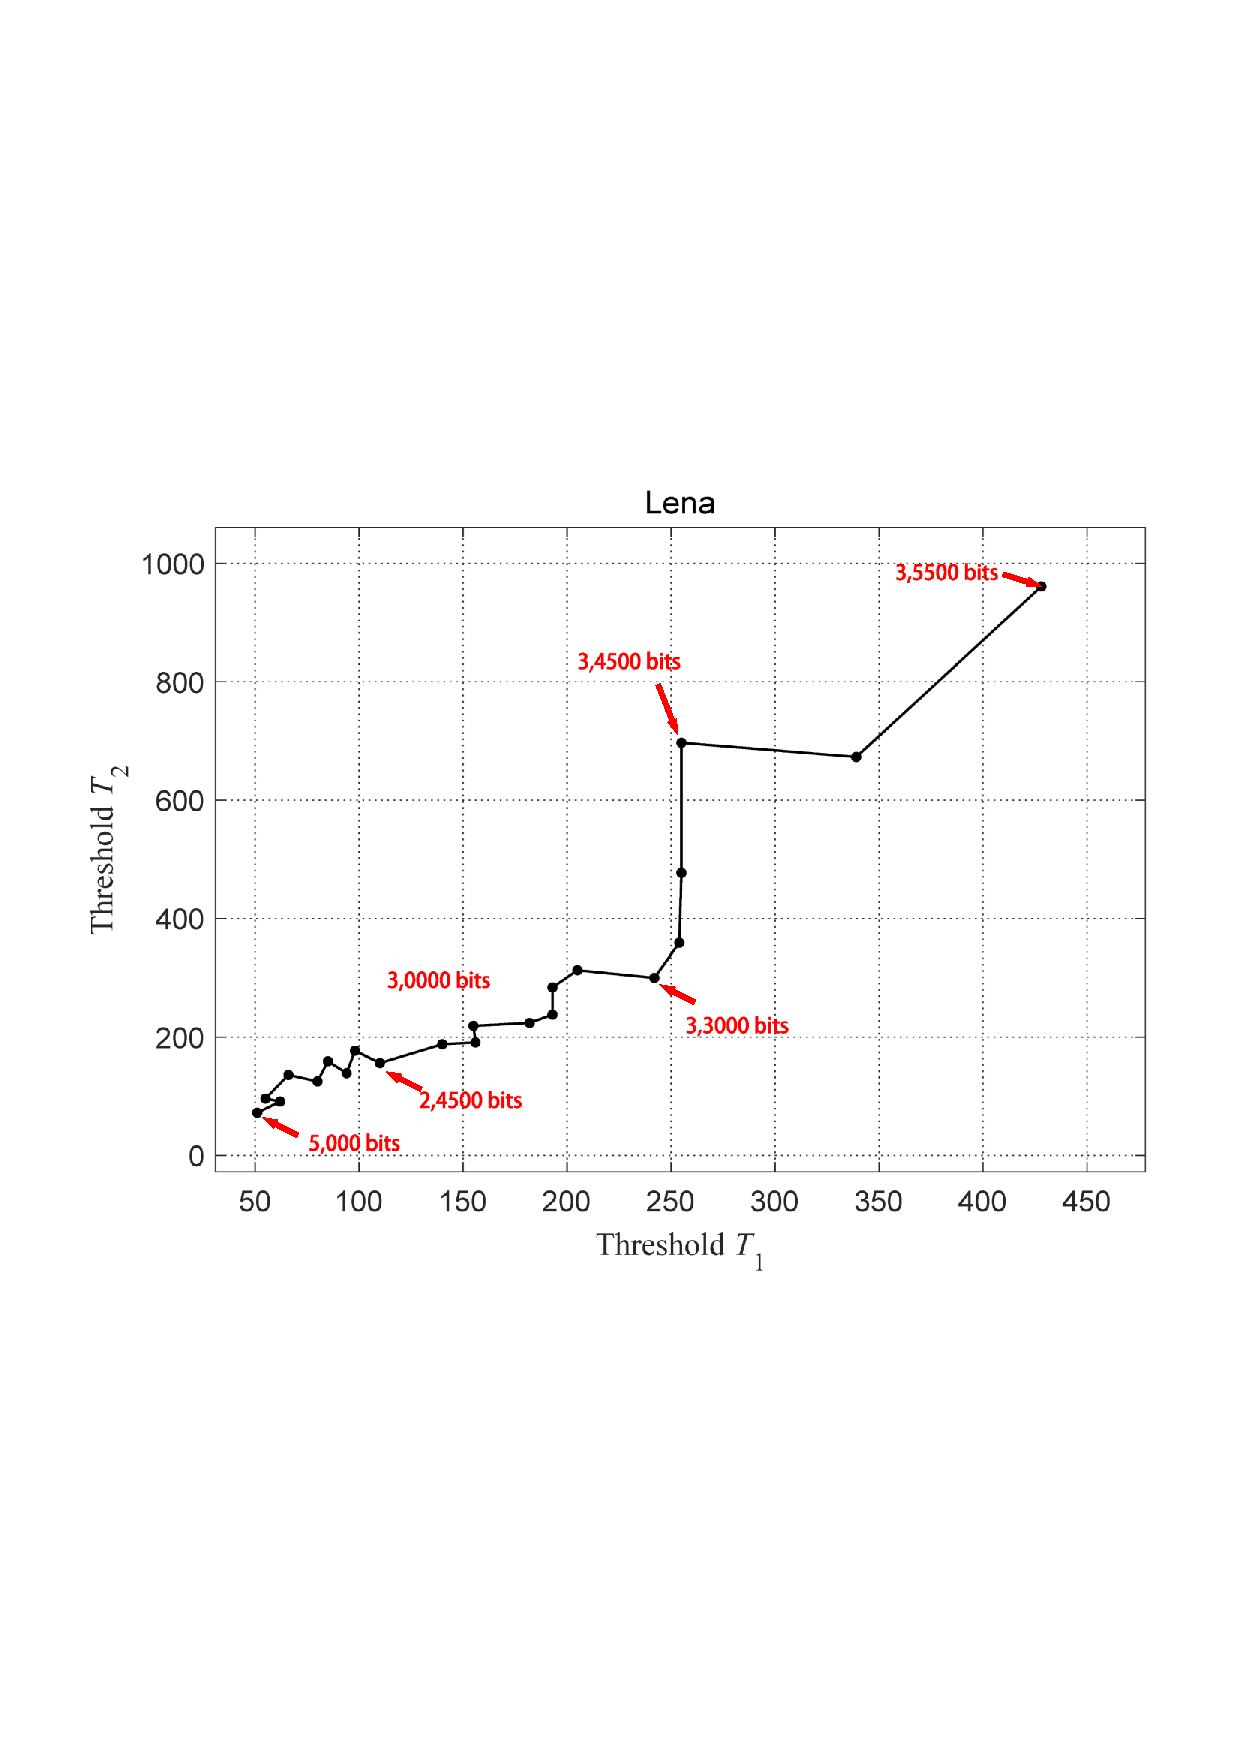
\includegraphics[width=0.5\textwidth]{figures/Thresholds.pdf}
\centering
\caption{Thresholds.}
\label{Fig.Thresholds}
\end{figure*}

\subsection{Data Embedding and Extraction Procedures}\label{sec:3.3}
The data embedding procedure is divided into the following steps to introduce as shown in Fig. \ref{Fig.Procedures}. Firstly, a location map ${\rm LM}$ is constructed to solve overflow/underflow problem. For $i$-th pixel $x_i$, if $x_i = 0$ or $x_i = 255$, we assign ${\rm LM}(i) = 1$. Otherwise, we assign ${\rm LM}(i) = 0$. All pixels equals $255$ are modified to $254$ and $0$ are modified to $1$. Because ${\rm LM}$ records all the locations where the overflow/underflow may occur, original pixels can be recovered. Next, for the given several context sizes $\{C_1, ..., C_N\}$ ($N$ is the number of context sizes), the complexity ${\rm NL}(i)$ of current pixel value $x_i$ is calculated the sum of the absolution differences of the horizontal and vertical of every two adjacent pixels belong to the largest size context $C_N$. And context pixels to predict $x_i$ are selected by comparing ${\rm NL}(i)$ with the given thresholds $\{T_1, ..., T_N\}$($0 \leq T_1 < T_2 < ... < T_N$ ), which is similar to the procedure described in section \ref{sec:3.2}. Then, $x_i$ is predicted by the chosen context pixels by (\ref{eq:EPPVOPE}) and one bit data is embedded by modifying $x_i$ to $\hat{x}_i$ by (\ref{eq:Embed}). The steps of prediction and embedding are performed pixel-by=pixel until all secret data is embedded and current pixel position is recorded as $k_{\rm end}$. Finally, for reversibility, some auxiliary information should be used for blind decoding such as
\begin{itemize}
  %\item number of context sizes $N$ (2 bits),
  \item the complexity thresholds $\{T_1, ..., T_N\}$ ($11 \times N$ bits),
  \item the pixel position where data embedding ends (18 bits),
  \item length of compressed location map $L$ (18 bits),
  \item the compressed location map ${\rm LM}$ ($L$ bits).
\end{itemize}
To embed the auxiliary information, LSB of first $36 + 11 \times N + L$ bits pixels of the image is recorded to obtain a binary vector $V_{\rm LSB}$ and then replaced by the auxiliary information. $V_{\rm LSB}$ is embedded into pixels after $x_{k_{\rm end}}$ by the same method by (\ref{eq:Embed}) at last.
During the whole embedding procedure, the threshold $T_1$ is selected from 1 and increased by 1 iteratively and $j$-th threshold $T_j$ is selected from $T_{j-1} + 1$ and increased by 1 iteratively. The optimal thresholds are obtained by traversing all values of pixel complexities.

The extraction procedure is an opposite process as shown in Fig. \ref{Fig.Procedures}. Firstly, auxiliary information is gotten by reading LSB of first $38 + 11 \times N + L$ bits pixels and replaced by LSB of pixels after $x_{k_{\rm end}}$. Next, for marked pixel value $\hat{x}$, complexity is computed as the same as embedding procedure by extracting data pixel-by-pixel in reverse order. And, with extracted $N$ complexity thresholds $\{T_1, ..., T_N\}$, the same context pixels $C$ of $\hat{x}$ as original pixel value $x$ can be obtained. Then, prediction-error $\hat{p}$ of the marked pixel value $\hat{x}$ is computed by
\begin{equation}\label{eq:EPPVODPE}
\hat{p} = \left\{\begin{array}{ll}
\hat{x} - \max(C),      & \text{if } x \in S_1  \\
\min(C) - \hat{x},      & \text{if } x \in S_2 \cup S_3 \\
0,                      & \text{if } x \in S_4 \\
\hat{x} - \max(C) - 1,  & \text{if } x \in S_5  \\
{\rm skip},             & \text{otherwise}
\end{array}\right..
\end{equation}
The original pixel value $x$ is recovered by
\begin{equation}\label{eq:EPPVOdMPixel}
x = \left\{\begin{array}{ll}
\hat{x},        & \text{if } \hat{p} = 0 \\
\hat{x} - 1,    & \text{if } \hat{x} \in S_1 \cup S_4 \cup S_5 \text{ and } \hat{p} \geq 1 \\
\hat{x} + 1,    & \text{if } \hat{x} \in S_2 \cup S_3 \text{ and } \hat{p} \geq 1 \\
{\rm skip},         & \text{otherwise}
\end{array}\right..
\end{equation}
Meanwhile, the secret data $b$ equals 1 if $\hat{p}=1$ or $0$ if $\hat{p} = 0$. Finally, original image is recovered by ${\rm LM}$ referring the embedding procedure. The flowchart of extraction procedure is shown in Fig. \ref{Fig.Procedures}.

\begin{figure*}
\centering
\includegraphics[width=0.85\textwidth]{figures/Procedures.pdf}
\centering
\caption{Procedures.}
\label{Fig.Procedures}
\end{figure*}

%----------------------------------------------------------------------------------------
\section{Experimental Results}\label{sec:4}
% N \in {1, 2, 3, 4}, N=4 been chosen,
In this section, experimental results of proposed method are presented. The performance is compared with three typical PVO-based methods of Peng \emph{et al.} \cite{Peng2014IPVO}, Ou \emph{et al.} \cite{Ou2014PVOk} and Qu \emph{et al.} \cite{Qu2015PPVO}. The proposed method is implemented on MatLab version 2018a on a tower server (SUPERMICRO LT-7038AX) and for a given embedding capacity, embedding procedure can be implemented less than four seconds. The experimental results are evaluated on eight standard gray-scale $512 \times 512$-sized images including Lena, Baboon, Airplane, Barabra, Lake, Boat, Peppers and Eliane.

Firstly, we consider the impact of number $N$ of context sizes to the embedding capacity. As shown in Fig. \ref{fig:size}, for each given capacity, $N$ is from $1$ to $4$, corresponding the sizes $C_1 \in \{C_1\}$, $C_{12} \in \{C_1, C_2\}$, $C_{123} \in \{C_1, C_2, C_3\}$ and $C_{1234} \in \{C_1, C_2, C_3, C_4\}$, respectively. It shows that although the embedding performance increases with the increase of $N$, it is already very small when $N = 4$. Therefore, balancing the embedding performance and embedding time complexity, we set $N = 4$ as a suitable size number. There are four complexity thresholds $\{T_1, T_2, T_3, T_4\}$ to choose context pixels for the current pixel, and the smoother the area where the pixel is, the less context pixels are used to predict.

Next, Fig. \ref{fig:size} shows the performance comparison on the eight test images. The capacity increases from 5,000 bits to the largest embedding capacity with a step of 1,000 bits. The figures reveal that the proposed method is superior to other three PVO-basd methods. Specifically, the performance comparison for given capacities of 10,000 bits and 20,000 bits are represented in Table~\ref{tab:10000bits} and Table~\ref{tab:20000bits}.

The improved PVO-based RDH proposed by Peng \emph{et al.} \cite{Peng2014IPVO} is an improvement of the original PVO RDH \cite{Li2013PVO}, the smooth blocks are utilized for data embedding by considering the original order of pixels in each block. Fig. \ref{fig:size} shows that its performance is mediocre compared with other methods. Through Table~\ref{tab:10000bits} and Table~\ref{tab:20000bits}, the proposed method obtain an improvement of PSNR of 0.93 dB and 1.0 dB respectively. The PVO-$k$ proposed by Qu \emph{et al.} \cite{Qu2015PPVO} is another RDH method which aims to make full use of smooth blocks as well. In this method, the blocks with more than one largest/smallest pixel value are utilized by modifying the largest/smallest pixel values concurrent. It shows a better performance than the improved PVO-based method but it is still unsatisfactory. According to Table~\ref{tab:10000bits} and Table~\ref{tab:20000bits}, the proposed method obtain an improvement of PSNR of 0.66 dB and 0.79 dB respectively.

The PPVO RDH proposed by Qu \emph{et al.} \cite{Qu2015PPVO} is different from traditional PVO-based RDH methods. It breaks through the block constraint and prediction process is implemented pixel by pixel. In this method, whatever the pixel is in a smooth or complex area, the context pixels for prediction is constant. The performance of PPVO achieve a superior performance than traditional PVO-based RDH methods. According to the Table~\ref{tab:10000bits} and Table~\ref{tab:20000bits}, the proposed method considers the impact of the number of context pixels and get a increase of PSNR of 0.60 dB and 0.14 dB respectively.

\begin{figure*}
\centering
\subfigure{
\begin{minipage}[t]{0.39\linewidth}
\centering
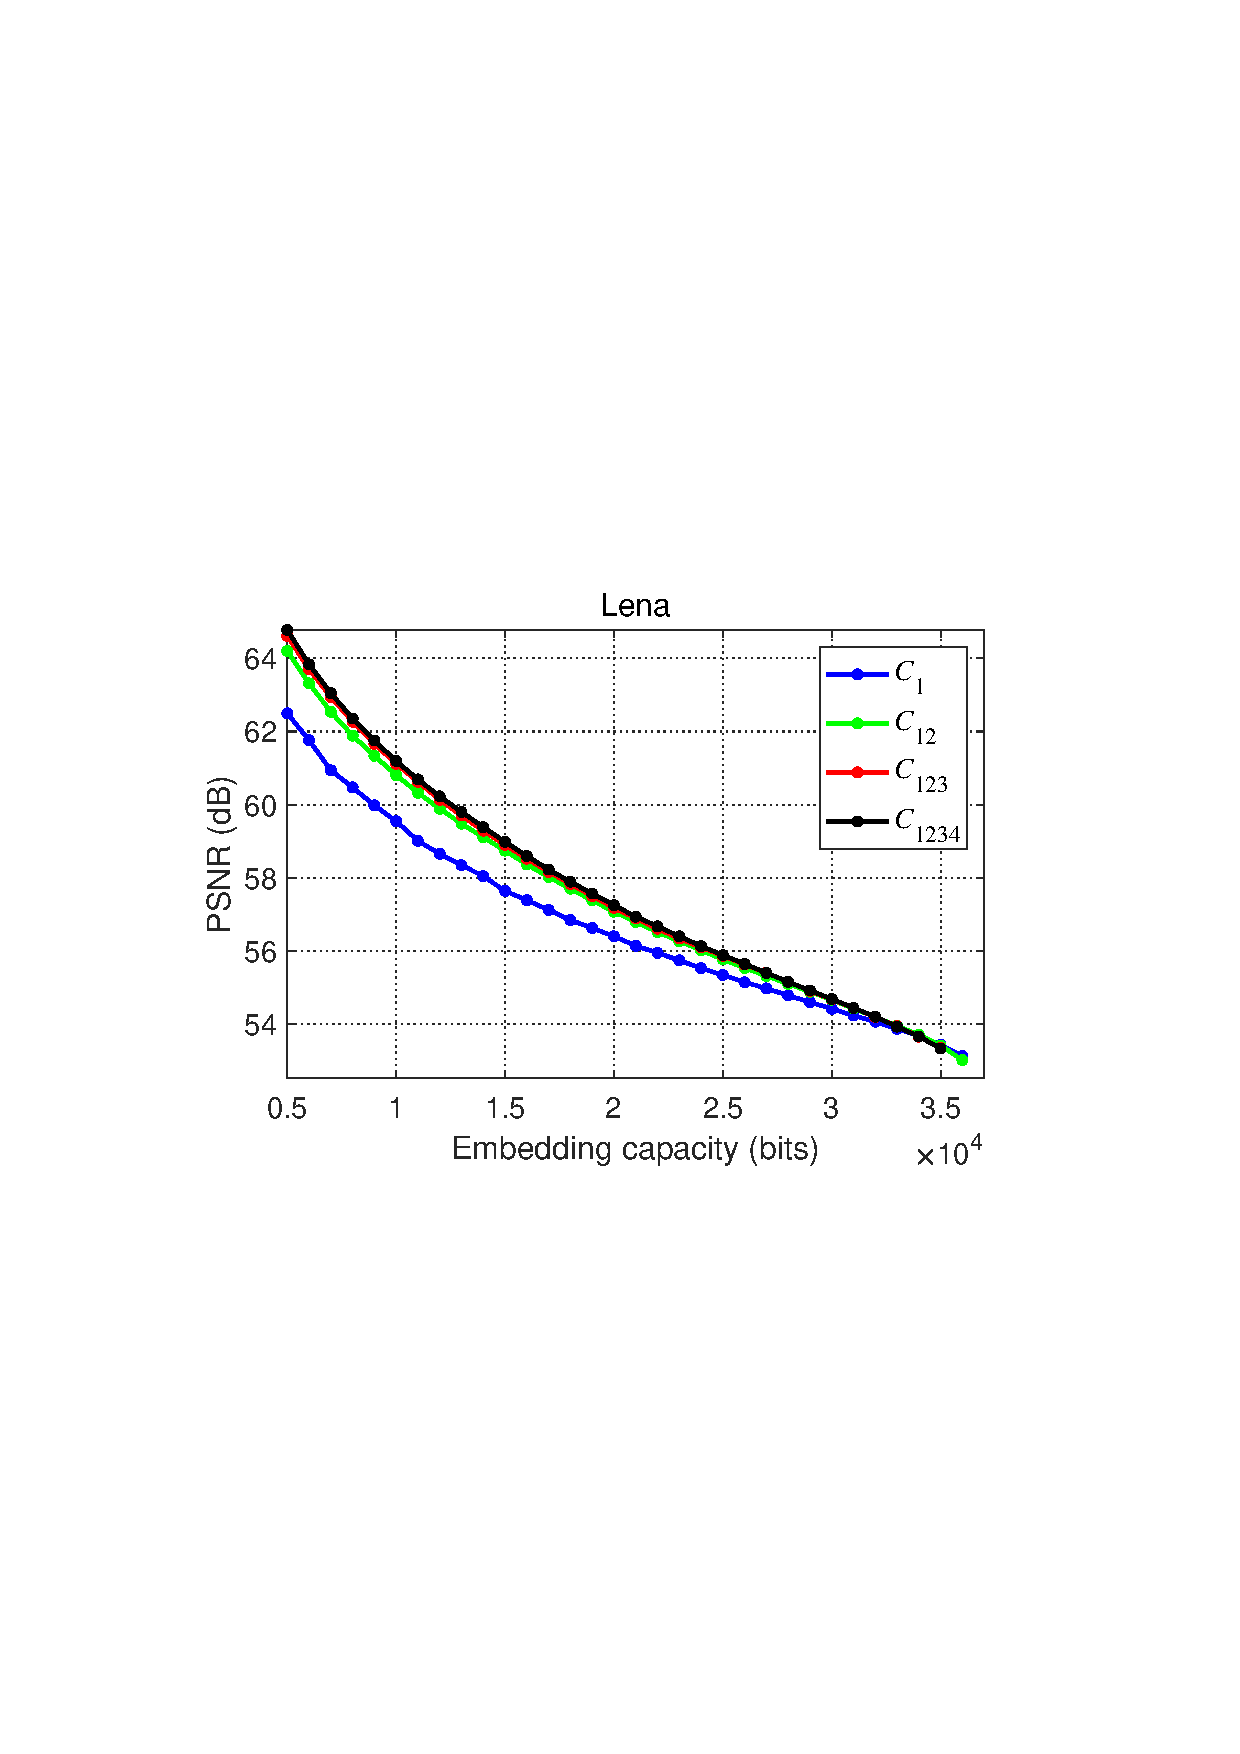
\includegraphics[width=1\textwidth]{figures/Result/size/Lena.pdf}
\end{minipage}
}
\qquad
\subfigure{
\begin{minipage}[t]{0.4\linewidth}
\centering
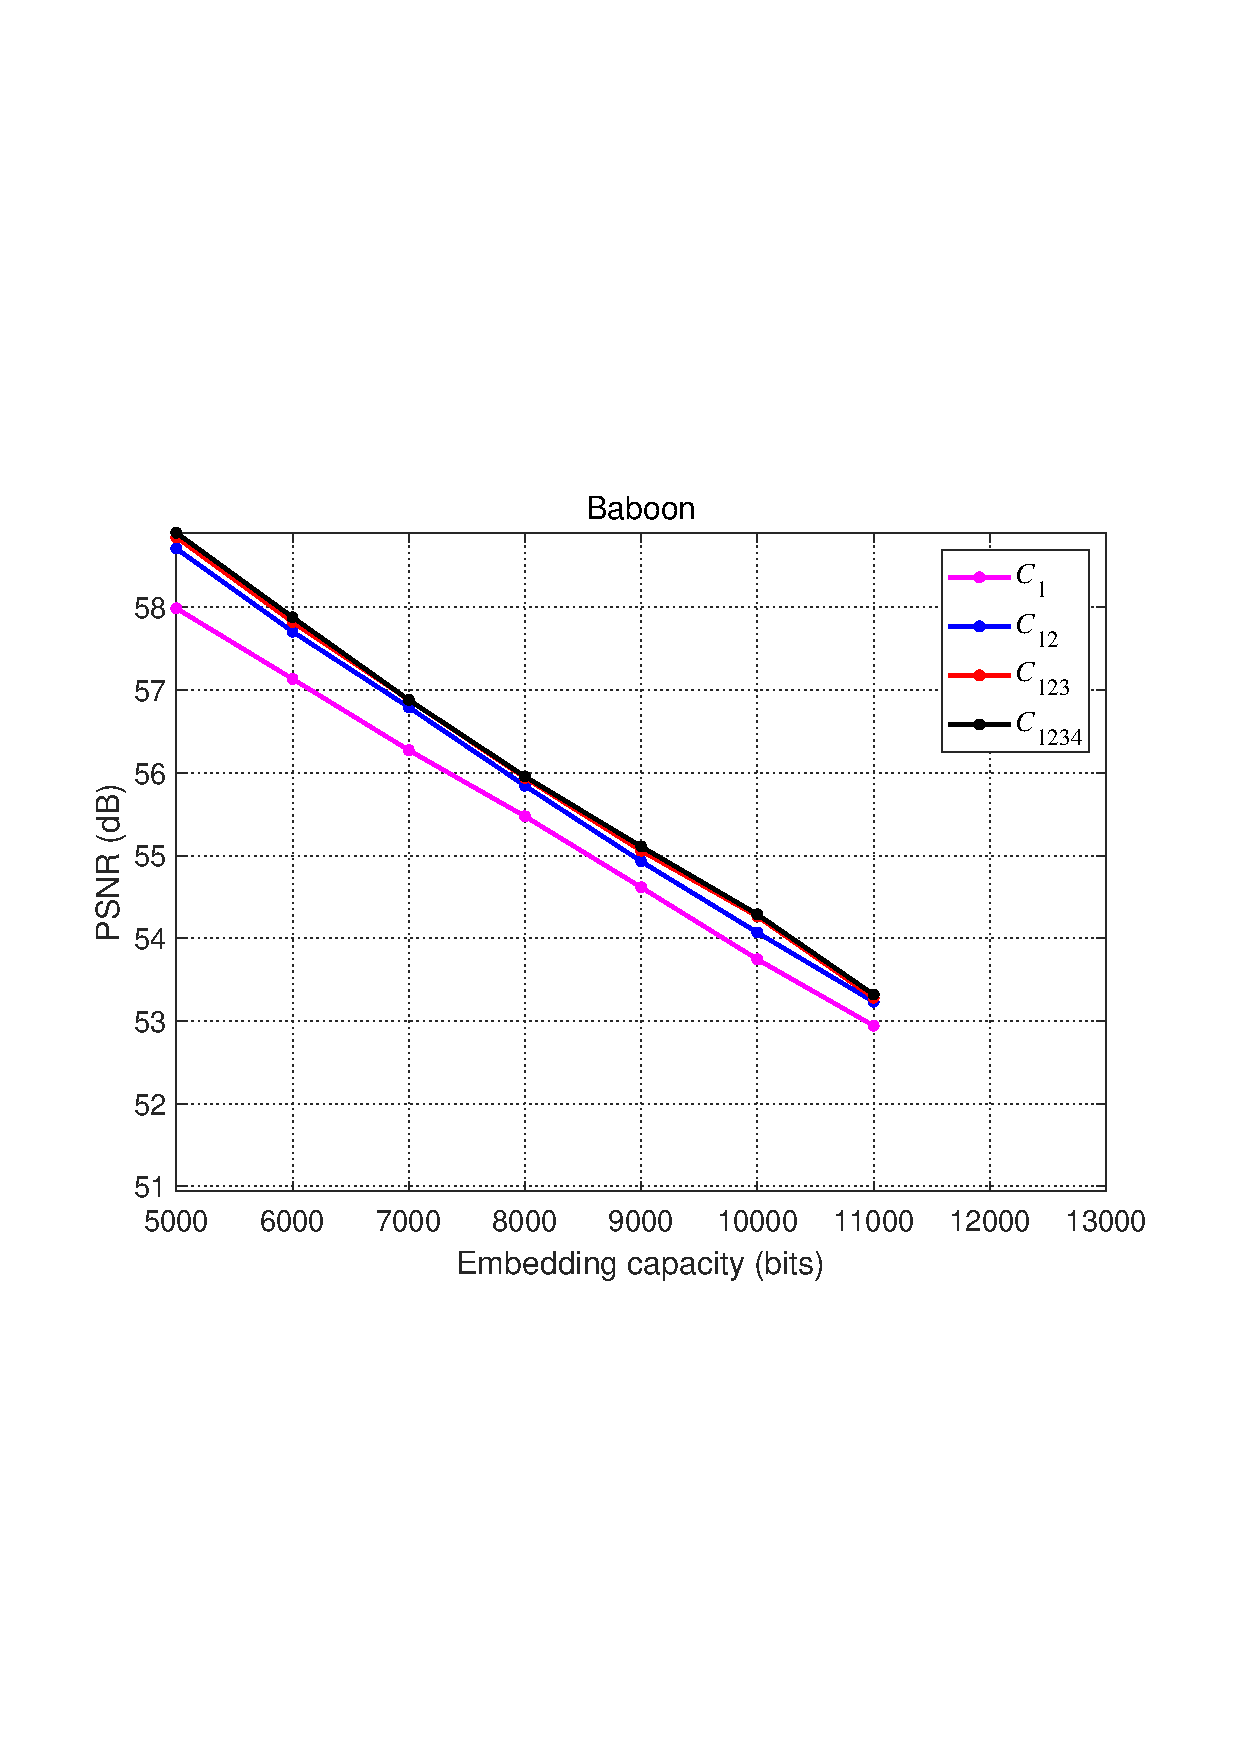
\includegraphics[width=1\textwidth]{figures/Result/size/Baboon.pdf}
\end{minipage}
}

\subfigure{
\begin{minipage}[t]{0.39\linewidth}
\centering
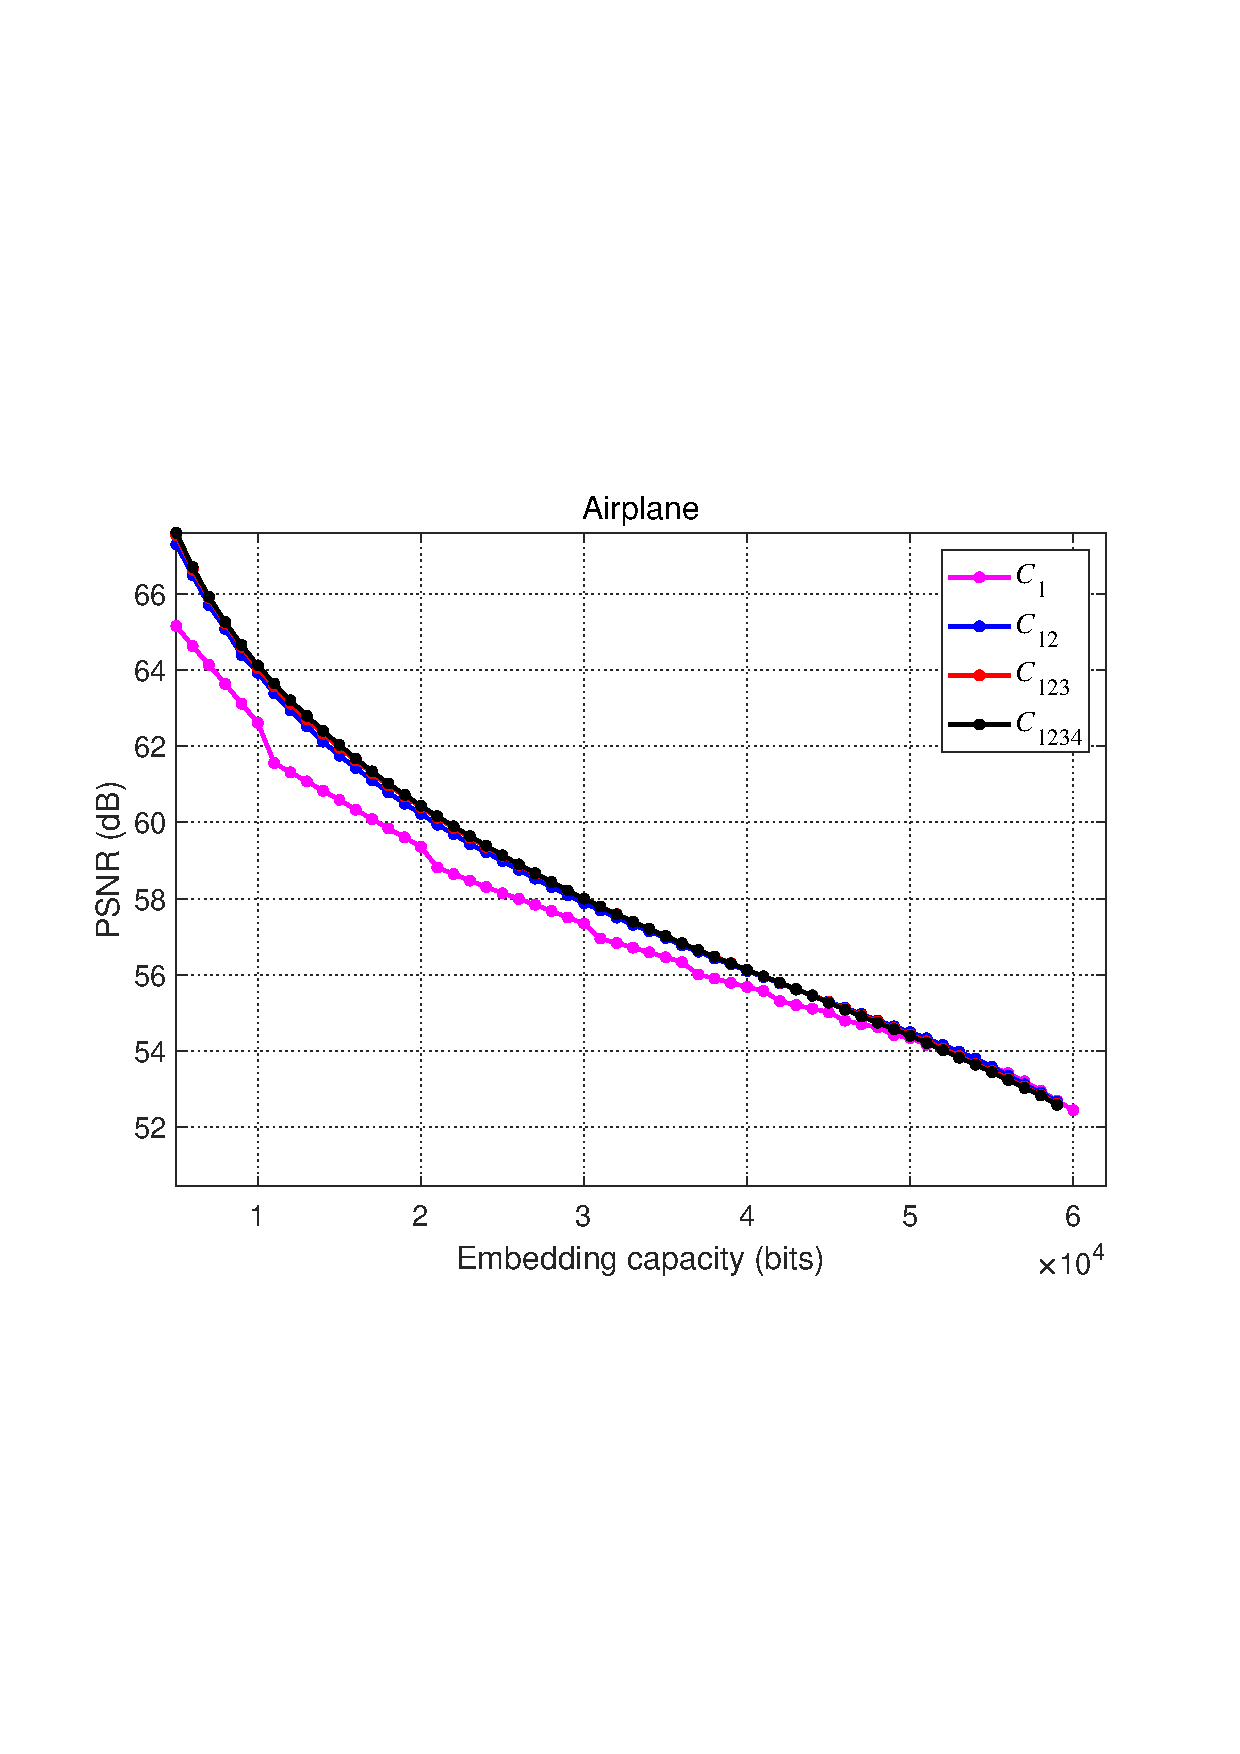
\includegraphics[width=1\textwidth]{figures/Result/size/Airplane.pdf}
\end{minipage}
}
\qquad
\subfigure{
\begin{minipage}[t]{0.39\linewidth}
\centering
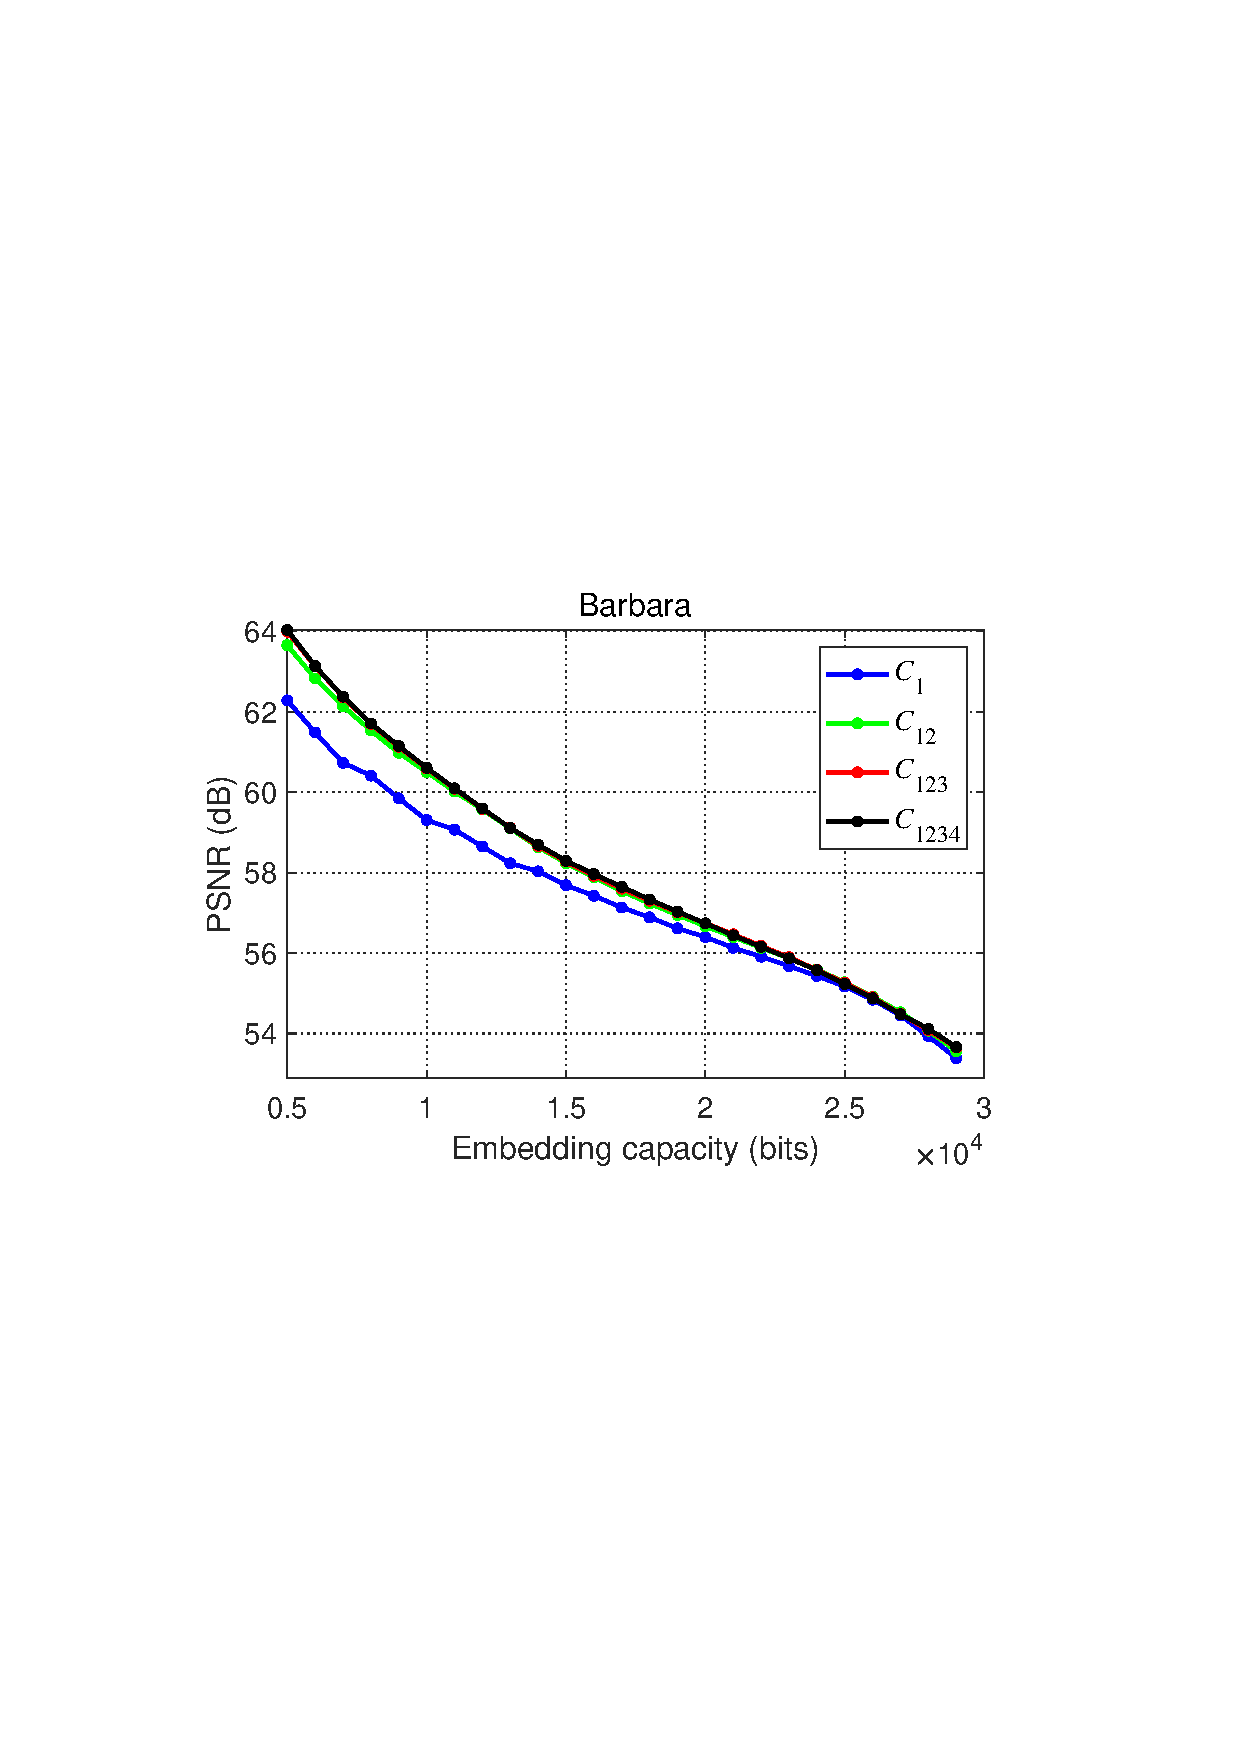
\includegraphics[width=1\textwidth]{figures/Result/size/Barbara.pdf}
\end{minipage}
}

\subfigure{
\begin{minipage}[t]{0.39\linewidth}
\centering
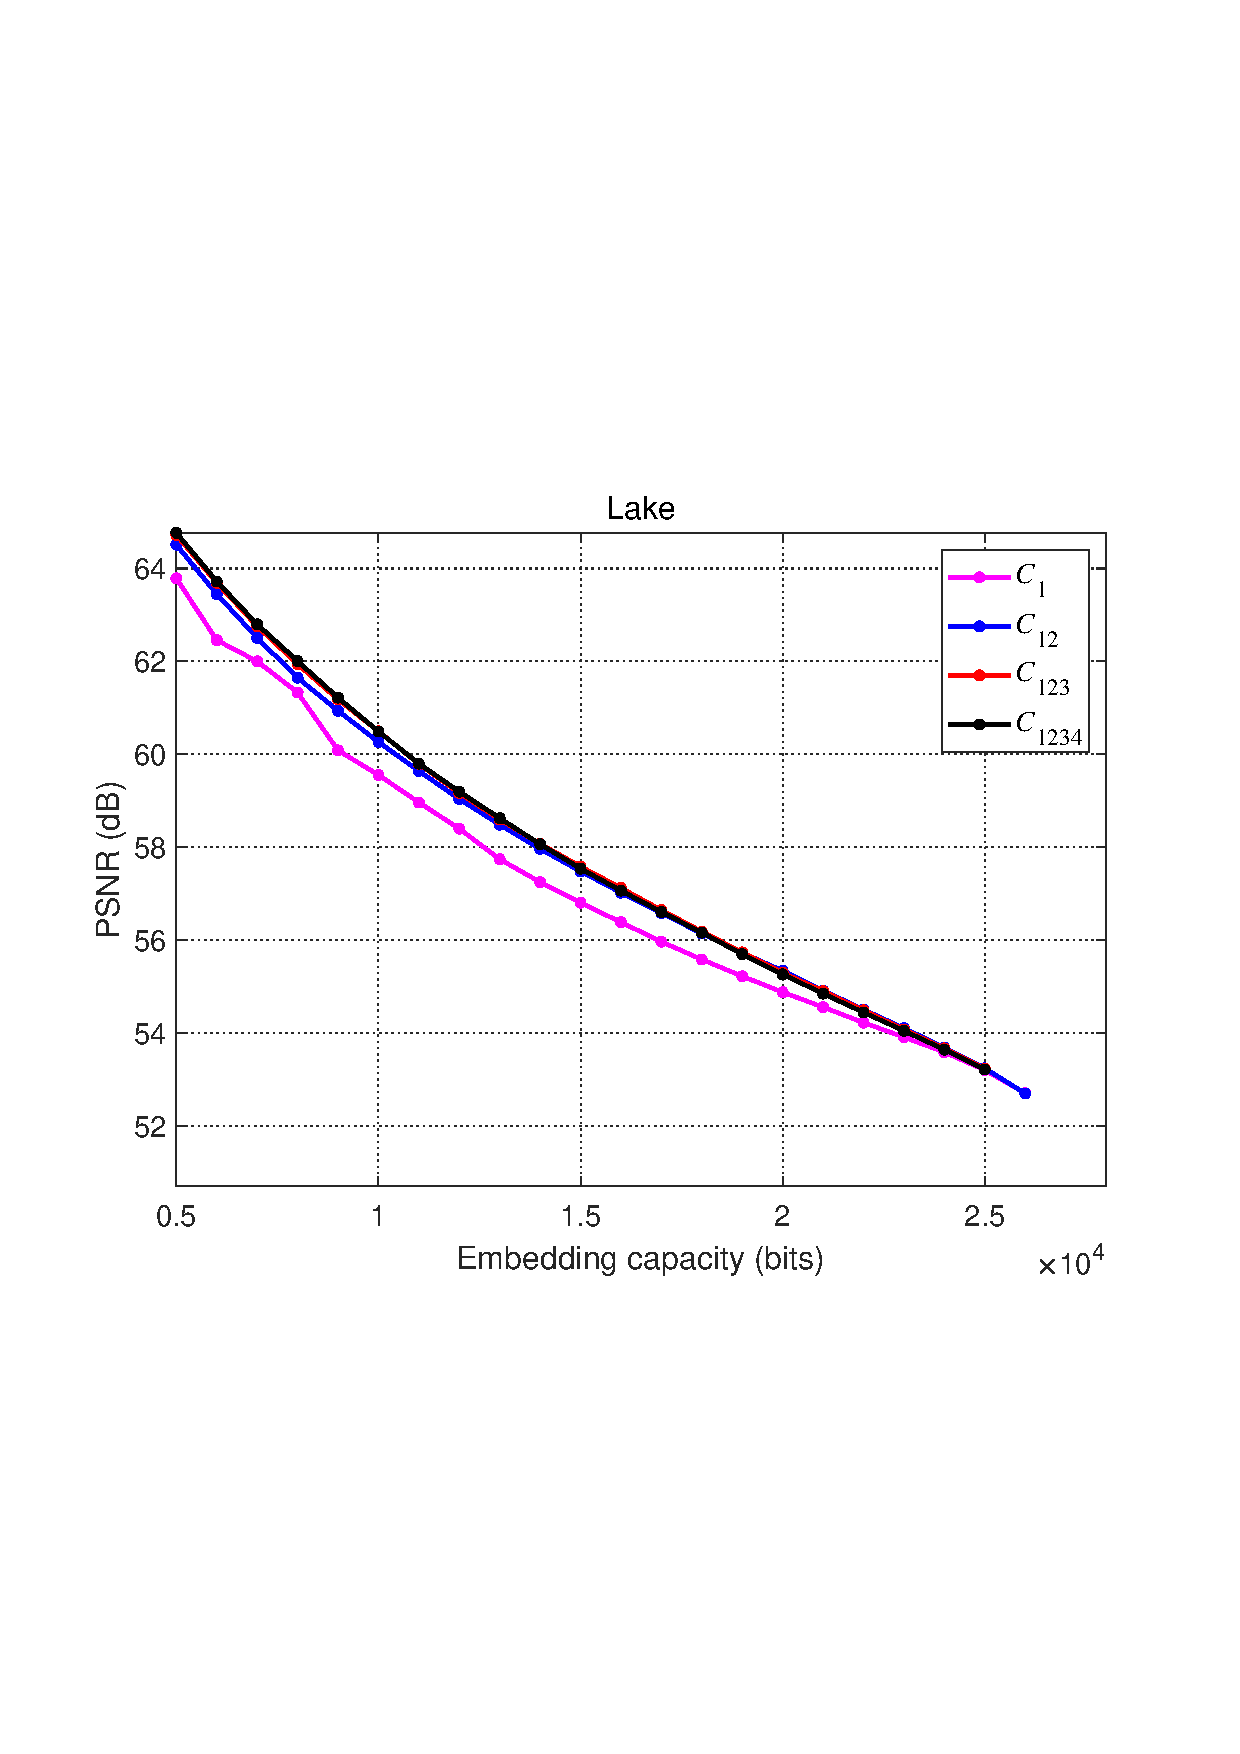
\includegraphics[width=1\textwidth]{figures/Result/size/Lake.pdf}
\end{minipage}
}
\qquad
\subfigure{
\begin{minipage}[t]{0.39\linewidth}
\centering
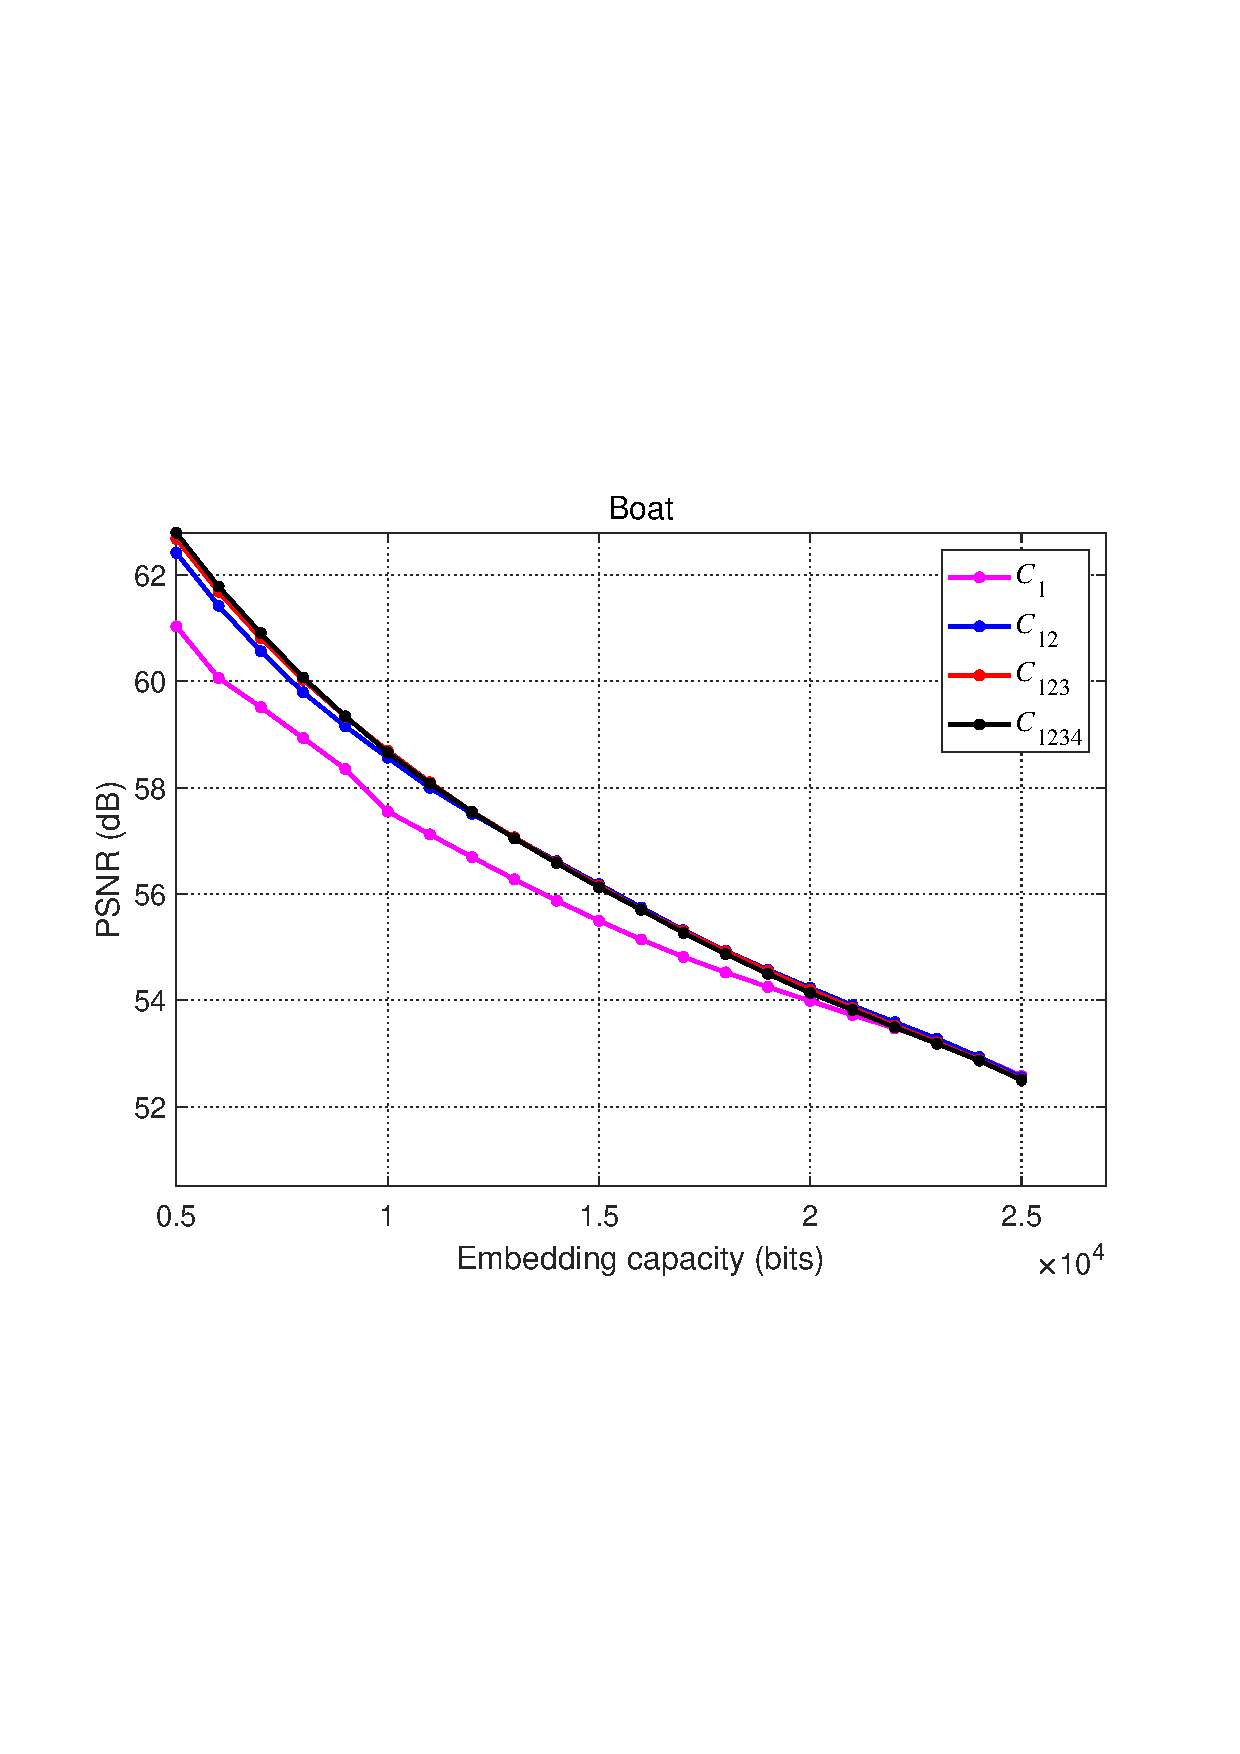
\includegraphics[width=1\textwidth]{figures/Result/size/Boat.pdf}
\end{minipage}
}

\subfigure{
\begin{minipage}[t]{0.39\linewidth}
\centering
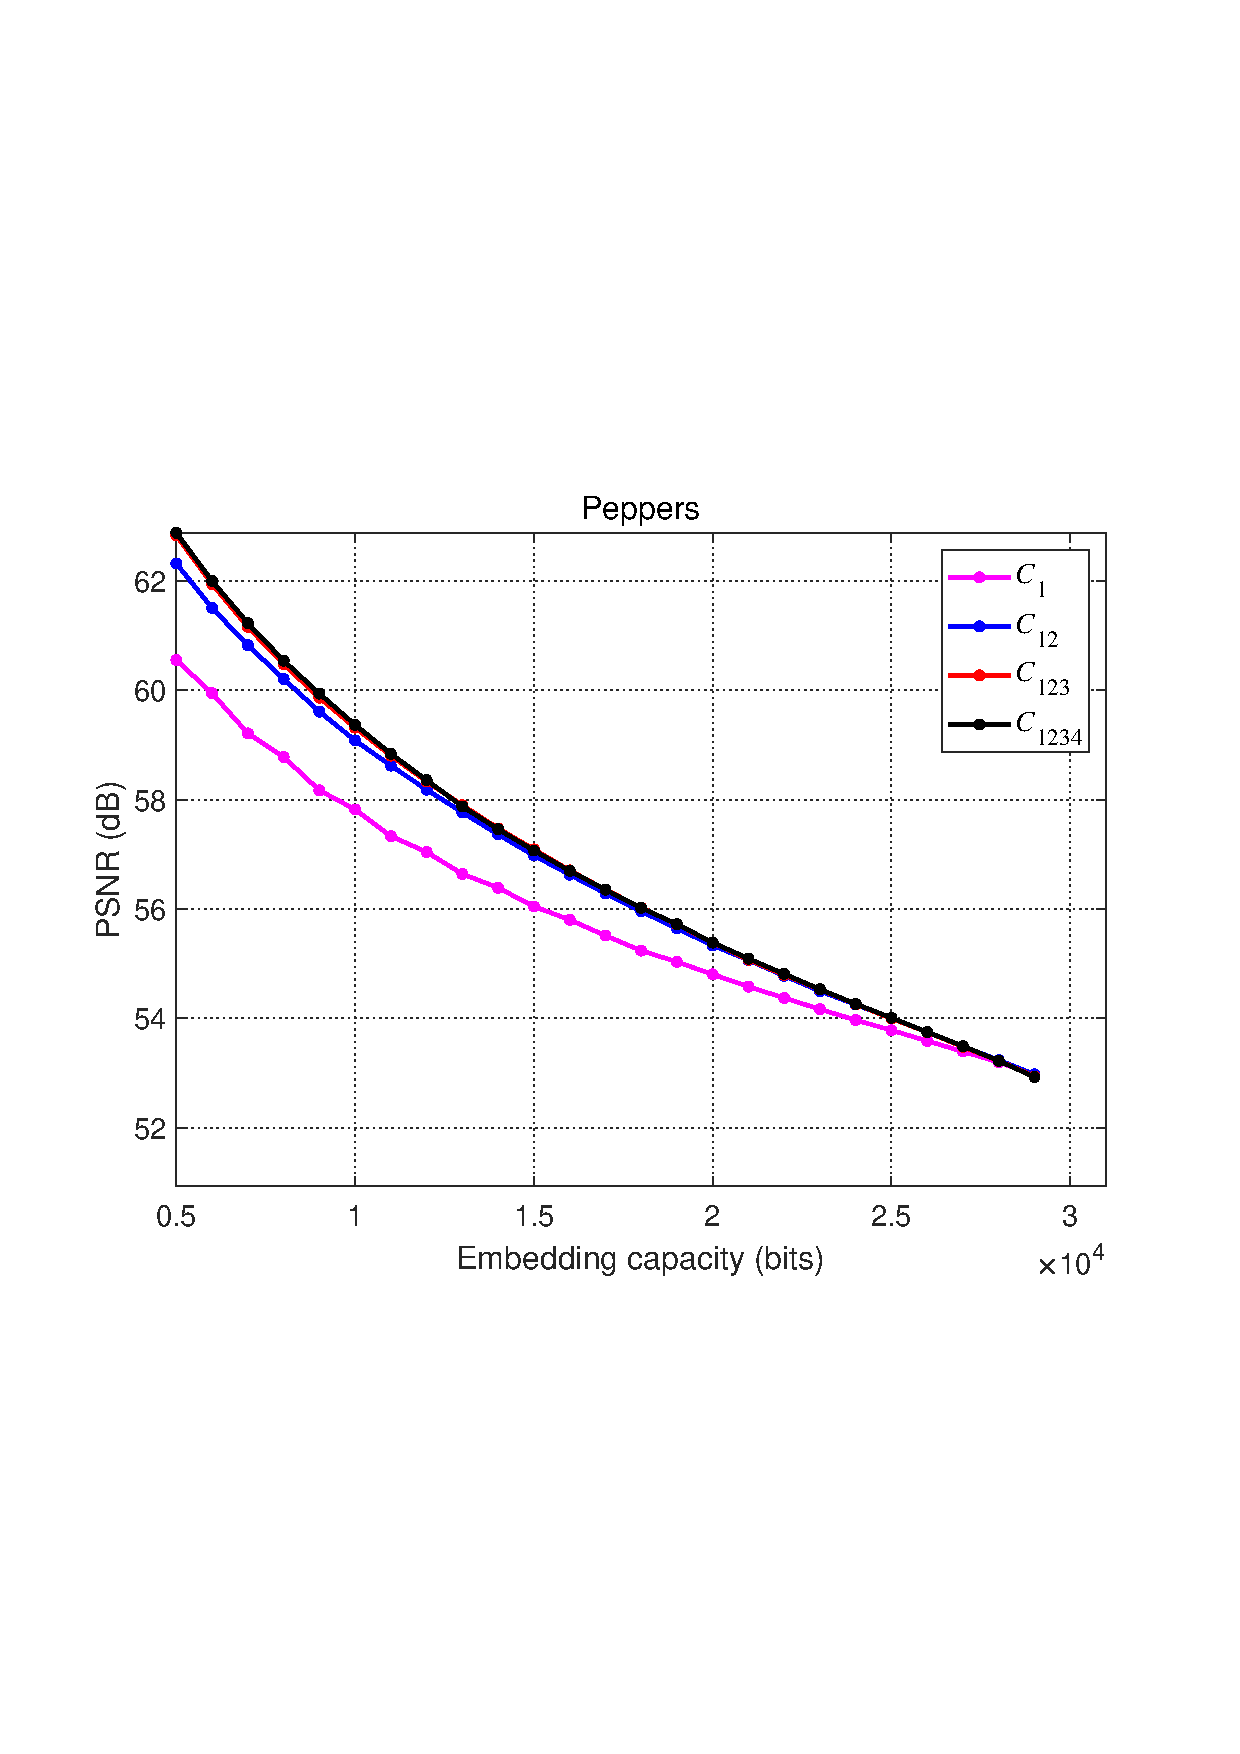
\includegraphics[width=1\textwidth]{figures/Result/size/Peppers.pdf}
\end{minipage}
}
\qquad
\subfigure{
\begin{minipage}[t]{0.39\linewidth}
\centering
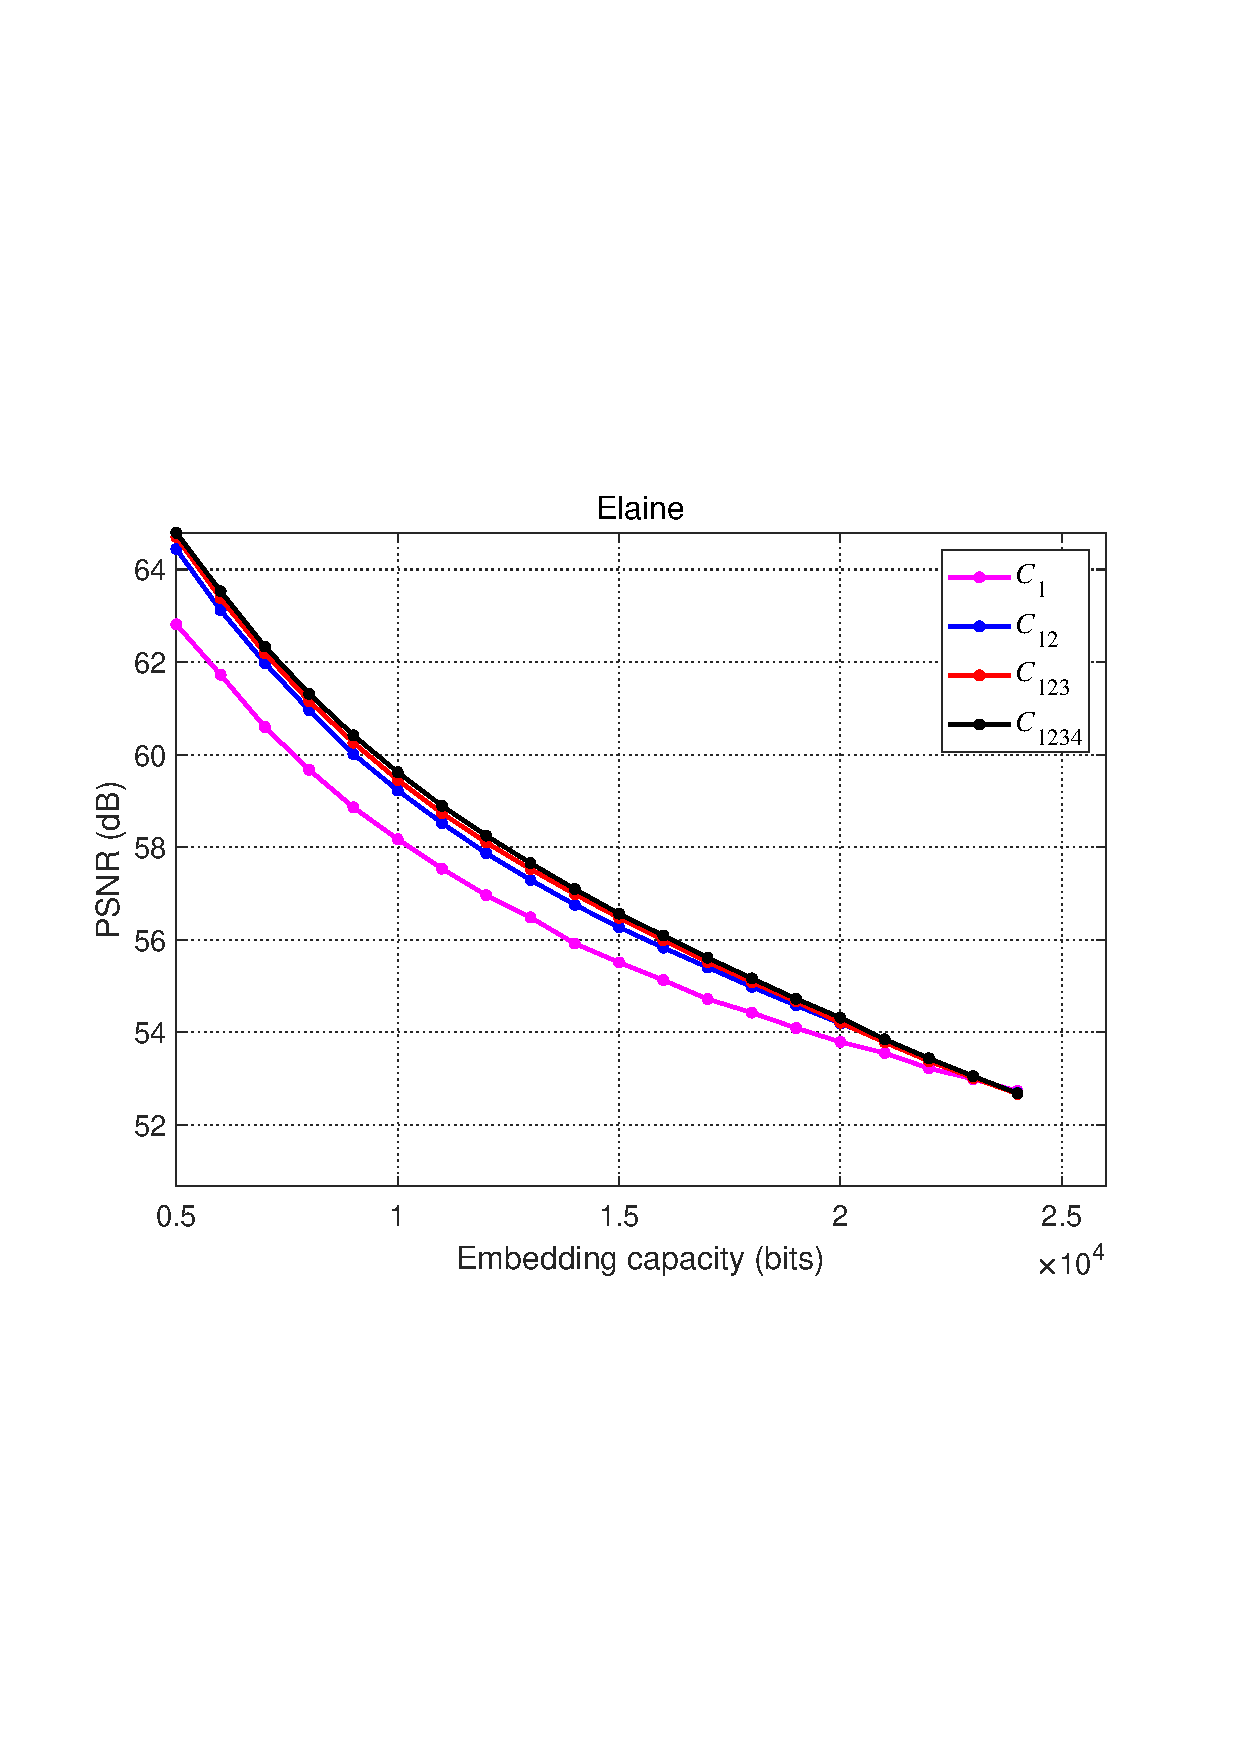
\includegraphics[width=1\textwidth]{figures/Result/size/Elaine.pdf}
\end{minipage}
}
\centering
\caption{size.}
\label{fig:size}       % Give a unique label
\end{figure*}


\begin{figure*}
\centering
\subfigure{
\begin{minipage}[t]{0.415\linewidth}
\centering
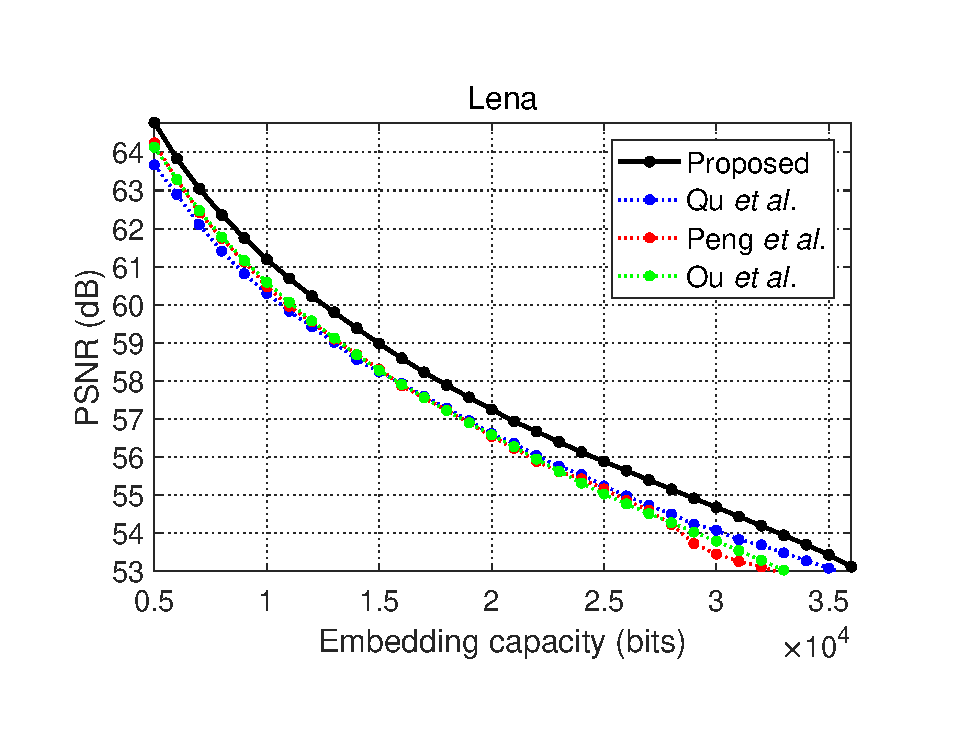
\includegraphics[width=1\textwidth]{figures/Result/capacity/Lena.pdf}
\end{minipage}
}
\subfigure{
\begin{minipage}[t]{0.43\linewidth}
\centering
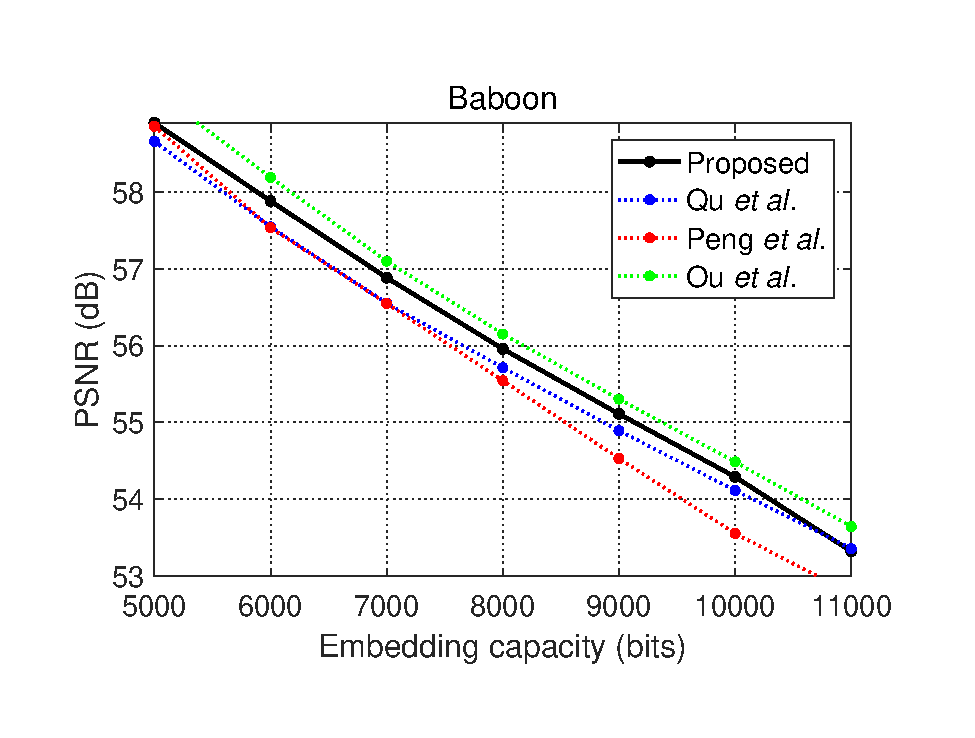
\includegraphics[width=1\textwidth]{figures/Result/capacity/Baboon.pdf}
\end{minipage}
}

\subfigure{
\begin{minipage}[t]{0.415\linewidth}
\centering
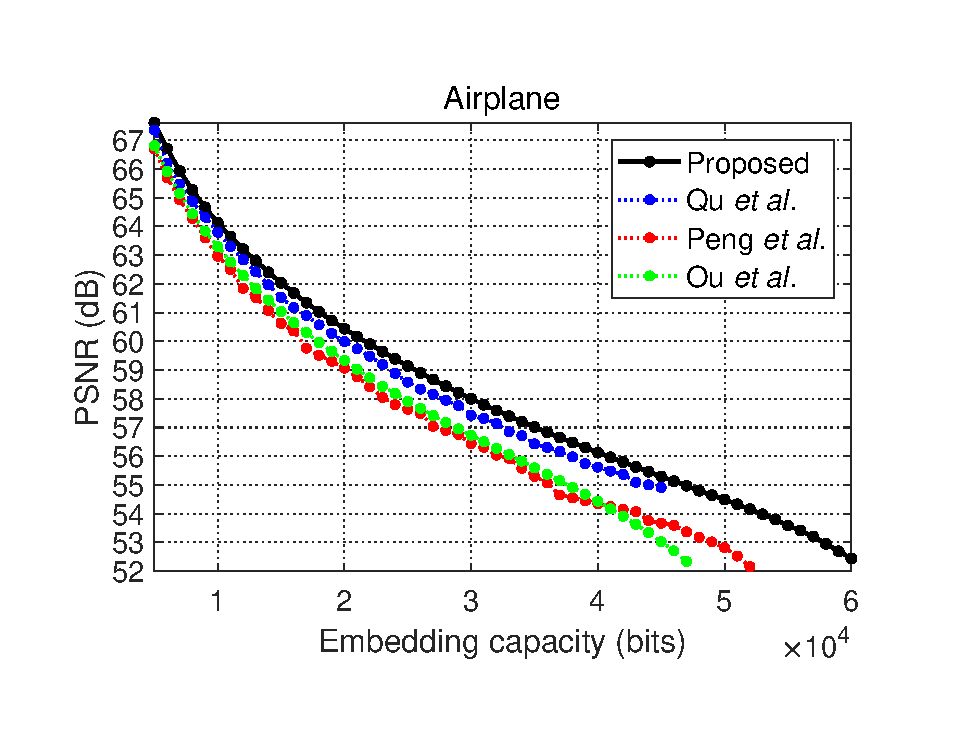
\includegraphics[width=1\textwidth]{figures/Result/capacity/Airplane.pdf}
\end{minipage}
}
\subfigure{
\begin{minipage}[t]{0.415\linewidth}
\centering
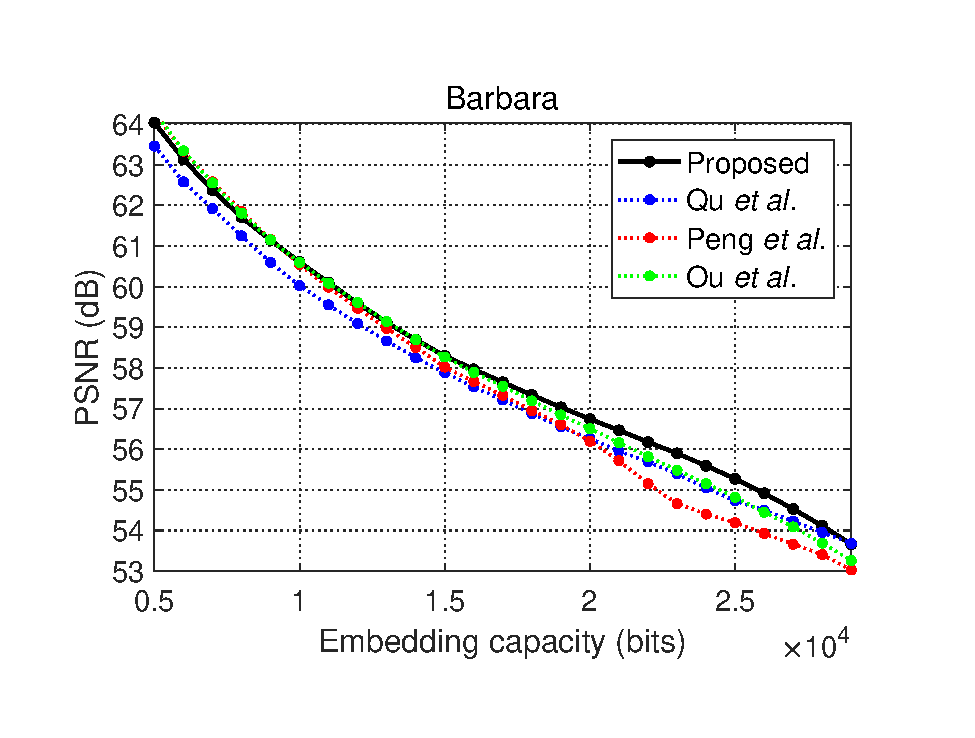
\includegraphics[width=1\textwidth]{figures/Result/capacity/Barbara.pdf}
\end{minipage}
}

\subfigure{
\begin{minipage}[t]{0.415\linewidth}
\centering
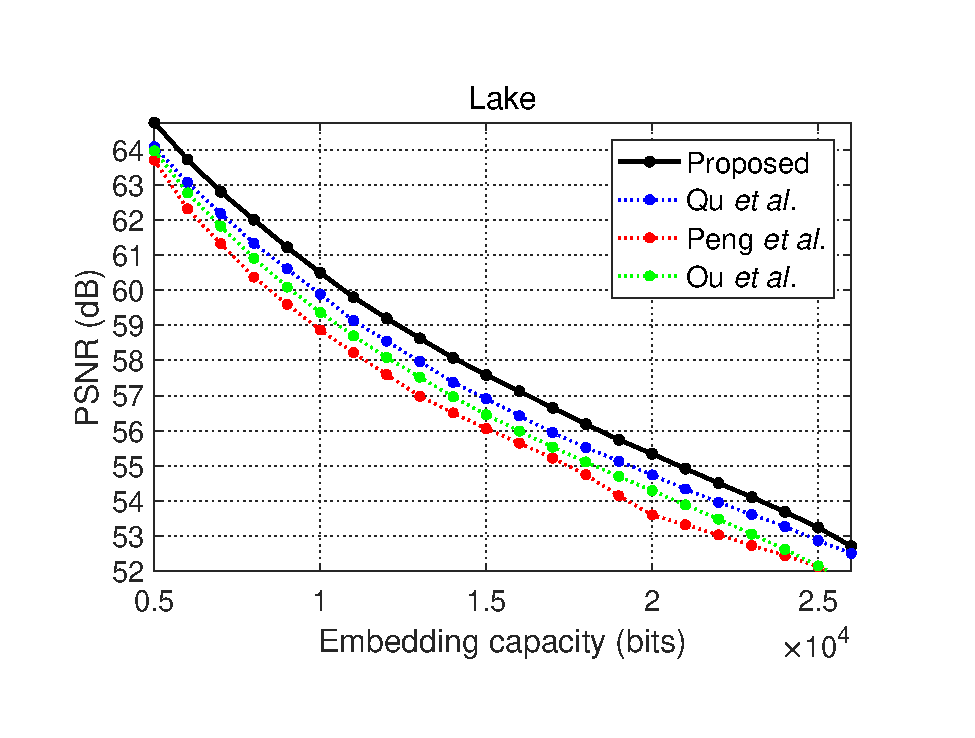
\includegraphics[width=1\textwidth]{figures/Result/capacity/Lake.pdf}
\end{minipage}
}
\subfigure{
\begin{minipage}[t]{0.42\linewidth}
\centering
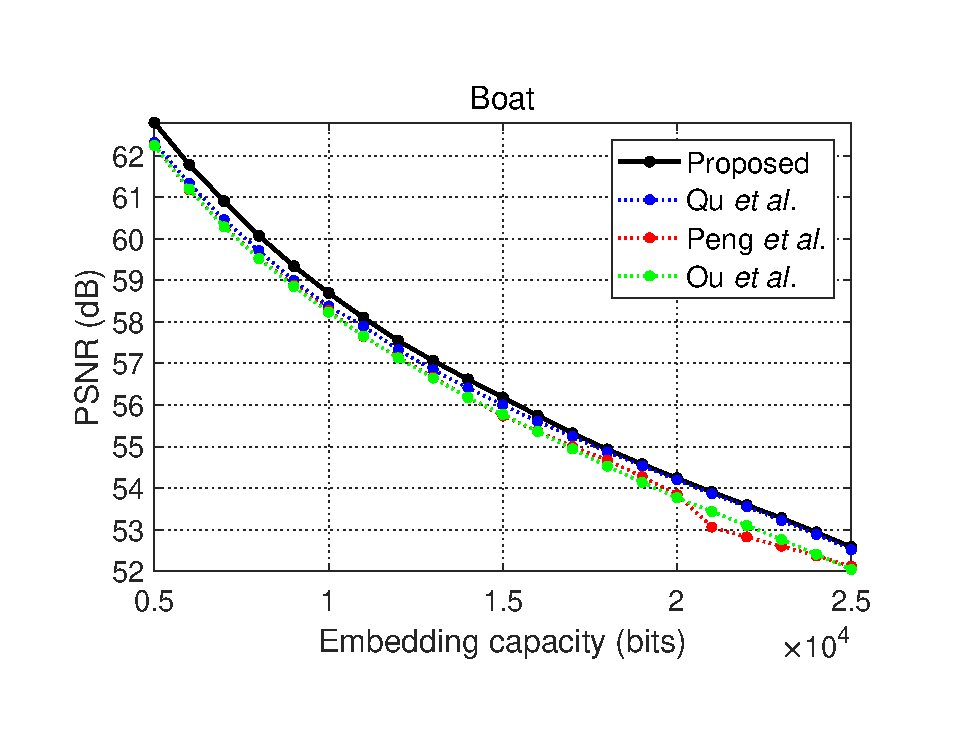
\includegraphics[width=1\textwidth]{figures/Result/capacity/Boat.pdf}
\end{minipage}
}

\subfigure{
\begin{minipage}[t]{0.415\linewidth}
\centering
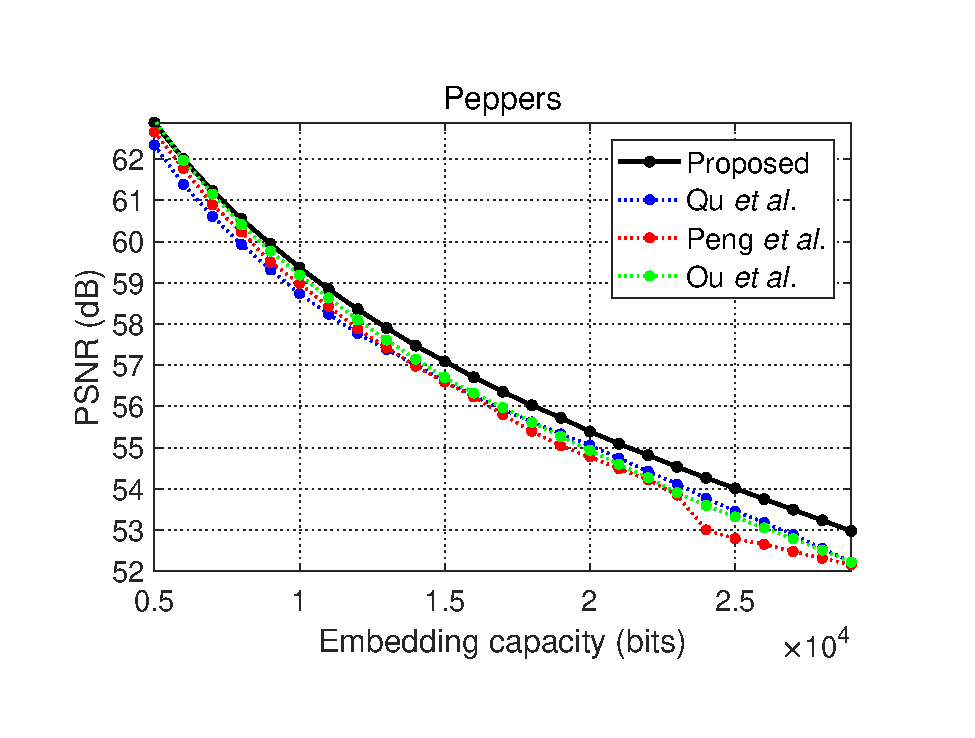
\includegraphics[width=1\textwidth]{figures/Result/capacity/Peppers.pdf}
\end{minipage}
}
\subfigure{
\begin{minipage}[t]{0.415\linewidth}
\centering
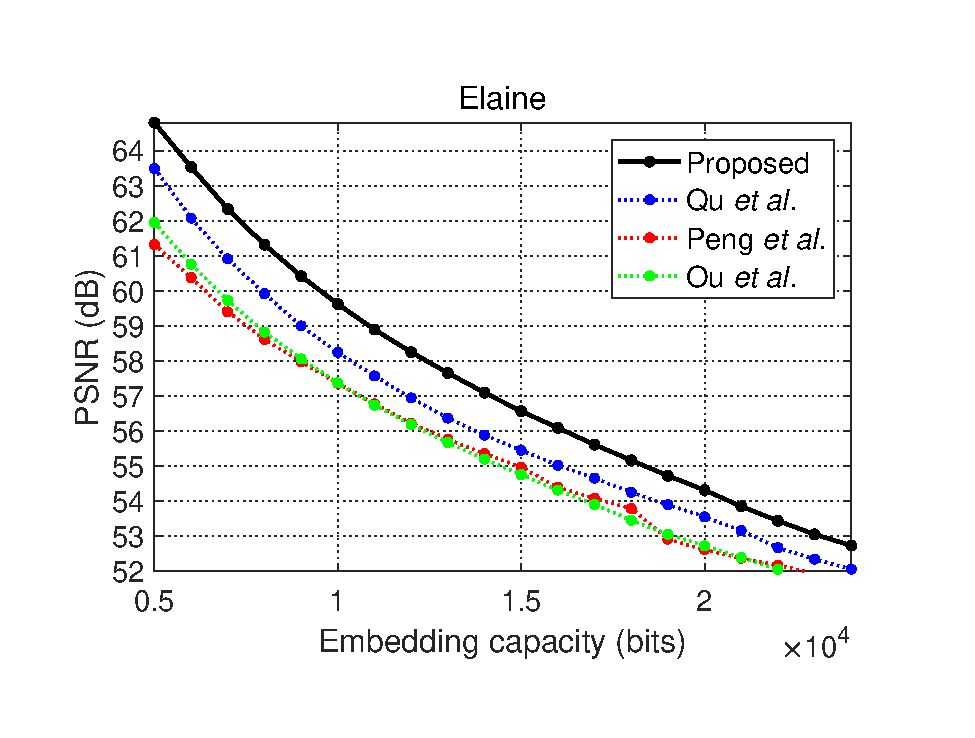
\includegraphics[width=1\textwidth]{figures/Result/capacity/Elaine.pdf}
\end{minipage}
}
\centering
\caption{capacity.}
\label{fig:capacity}       % Give a unique label
\end{figure*}

\begin{table}
\centering
\caption{Comparison of PSNR (dB) among the proposed method and the PVO-based methods of Peng \emph{et al.} \cite{Peng2014IPVO}, Ou \emph{et al.} \cite{Ou2014PVOk} and Qu \emph{et al.} \cite{Qu2015PPVO}. The embedding capacity is 10,000 bits.}
\setlength{\tabcolsep}{3mm}{
\begin{tabular}{lccccc}
\hline
{Images}                & Qu \emph{et al.}   & Peng \emph{et al.}    & Ou \emph{et al.}  & Proposed\\
\hline
Lena                    & 60.36              & 60.49                 & 60.59             & \textbf{61.19}\\ % 0.01
Baboon                  & 54.11              & 53.58                 & 54.48             & \textbf{54.29}\\ % 0.01
Airplane                & 63.76              & 62.97                 & 63.29             & \textbf{64.11}\\ % 0.01
Barbara                 & 60.08              & 60.48                 & 60.59             & \textbf{60.60}\\ % 0.01
Lake                    & 59.81              & 58.81                 & 59.36             & \textbf{60.47}\\ % 0.03
Boat                    & 58.37              & 58.26                 & 58.23             & \textbf{58.69}\\ % 0.01
Peppers                 & 58.73              & 58.97                 & 59.18             & \textbf{59.37}\\ % 0.01
Elaine                  & 58.30              & 57.37                 & 57.37             & \textbf{59.61}\\ % 0.02
\hline
Average                 & 59.19              & 58.86                 & 59.13             & \textbf{59.79}\\
\hline
\end{tabular}
}
\label{tab:10000bits}
\end{table}

\begin{table}
\centering
\caption{Comparison of PSNR (dB) among the proposed method and the PVO-based methods of Peng \emph{et al.} \cite{Peng2014IPVO}, Ou \emph{et al.} \cite{Ou2014PVOk} and Qu \emph{et al.} \cite{Qu2015PPVO}. The embedding capacity is 20,000 bits.}
\setlength{\tabcolsep}{3mm}{
\begin{tabular}{lccccc}
\hline
{Images}                & Qu \emph{et al.}   & Peng \emph{et al.}    & Ou \emph{et al.}  & Proposed\\
\hline
Lena                    & 56.65              & 56.56                 & 56.58             & \textbf{57.24}\\ % 0.01
Airplane                & 60.01              & 59.07                 & 59.33             & \textbf{60.39}\\ % 0.01
Barbara                 & 56.28              & 56.20                 & 56.50             & \textbf{56.74}\\ % 0.01
Lake                    & 54.71              & 53.53                 & 54.29             & \textbf{55.32}\\ % 0.03
Boat                    & 54.19              & 53.83                 & 53.76             & \textbf{54.24}\\ % 0.01
Peppers                 & 55.05              & 54.77                 & 54.93             & \textbf{55.37}\\ % 0.01
Elaine                  & 53.55              & 52.65                 & 52.71             & \textbf{54.30}\\ % 0.02
\hline
Average                 & 55.78              & 55.23                 & 55.44             & \textbf{56.23}\\
\hline
\end{tabular}
}
\label{tab:20000bits}
\end{table}

%----------------------------------------------------------------------------------------
\section{Conclusion}\label{sec:5}
In this paper, based on an extended PPVO predictor and multi-size based embedding method, an extended PPVO-based RDH method is proposed. For each pixel to be predicted, surrounding pixels in left lower and right lower direction are utilized to derive a sharper PEH. And next, the relationship between context region size and local complexity is explored. The pixels in smooth area are predicted by context pixels in a small region size. And for the pixels in complex area, context pixels are chosen by a larger region size. The proposed method is verified that is more satisfactory than other several state-of-the-art PVO-based RDH methods.

%----------------------------------------------------------------------------------------
\section*{Acknowledgement}
This work was supported by the National Key Research and Development of China (No. 2016YF-B0800404), the National Science Foundation of China (Nos. 61572052 and U1736213), and the Fundamental Research Funds for the Central Universities (Nos. 2017RC008 and 2018JBZ001).

\bibliographystyle{elsarticle-num}

\bibliography{Cited}


\end{document}
